% Options for packages loaded elsewhere
\PassOptionsToPackage{unicode}{hyperref}
\PassOptionsToPackage{hyphens}{url}
%
\documentclass[
]{book}
\usepackage{lmodern}
\usepackage{amssymb,amsmath}
\usepackage{ifxetex,ifluatex}
\ifnum 0\ifxetex 1\fi\ifluatex 1\fi=0 % if pdftex
  \usepackage[T1]{fontenc}
  \usepackage[utf8]{inputenc}
  \usepackage{textcomp} % provide euro and other symbols
\else % if luatex or xetex
  \usepackage{unicode-math}
  \defaultfontfeatures{Scale=MatchLowercase}
  \defaultfontfeatures[\rmfamily]{Ligatures=TeX,Scale=1}
\fi
% Use upquote if available, for straight quotes in verbatim environments
\IfFileExists{upquote.sty}{\usepackage{upquote}}{}
\IfFileExists{microtype.sty}{% use microtype if available
  \usepackage[]{microtype}
  \UseMicrotypeSet[protrusion]{basicmath} % disable protrusion for tt fonts
}{}
\makeatletter
\@ifundefined{KOMAClassName}{% if non-KOMA class
  \IfFileExists{parskip.sty}{%
    \usepackage{parskip}
  }{% else
    \setlength{\parindent}{0pt}
    \setlength{\parskip}{6pt plus 2pt minus 1pt}}
}{% if KOMA class
  \KOMAoptions{parskip=half}}
\makeatother
\usepackage{xcolor}
\IfFileExists{xurl.sty}{\usepackage{xurl}}{} % add URL line breaks if available
\IfFileExists{bookmark.sty}{\usepackage{bookmark}}{\usepackage{hyperref}}
\hypersetup{
  pdftitle={Modul Praktikum - Pelatihan Analisis Spasial},
  pdfauthor={Anik Djuraidah, Rahma Anisa, Gerry Alfa Dito},
  hidelinks,
  pdfcreator={LaTeX via pandoc}}
\urlstyle{same} % disable monospaced font for URLs
\usepackage{color}
\usepackage{fancyvrb}
\newcommand{\VerbBar}{|}
\newcommand{\VERB}{\Verb[commandchars=\\\{\}]}
\DefineVerbatimEnvironment{Highlighting}{Verbatim}{commandchars=\\\{\}}
% Add ',fontsize=\small' for more characters per line
\usepackage{framed}
\definecolor{shadecolor}{RGB}{248,248,248}
\newenvironment{Shaded}{\begin{snugshade}}{\end{snugshade}}
\newcommand{\AlertTok}[1]{\textcolor[rgb]{0.94,0.16,0.16}{#1}}
\newcommand{\AnnotationTok}[1]{\textcolor[rgb]{0.56,0.35,0.01}{\textbf{\textit{#1}}}}
\newcommand{\AttributeTok}[1]{\textcolor[rgb]{0.77,0.63,0.00}{#1}}
\newcommand{\BaseNTok}[1]{\textcolor[rgb]{0.00,0.00,0.81}{#1}}
\newcommand{\BuiltInTok}[1]{#1}
\newcommand{\CharTok}[1]{\textcolor[rgb]{0.31,0.60,0.02}{#1}}
\newcommand{\CommentTok}[1]{\textcolor[rgb]{0.56,0.35,0.01}{\textit{#1}}}
\newcommand{\CommentVarTok}[1]{\textcolor[rgb]{0.56,0.35,0.01}{\textbf{\textit{#1}}}}
\newcommand{\ConstantTok}[1]{\textcolor[rgb]{0.00,0.00,0.00}{#1}}
\newcommand{\ControlFlowTok}[1]{\textcolor[rgb]{0.13,0.29,0.53}{\textbf{#1}}}
\newcommand{\DataTypeTok}[1]{\textcolor[rgb]{0.13,0.29,0.53}{#1}}
\newcommand{\DecValTok}[1]{\textcolor[rgb]{0.00,0.00,0.81}{#1}}
\newcommand{\DocumentationTok}[1]{\textcolor[rgb]{0.56,0.35,0.01}{\textbf{\textit{#1}}}}
\newcommand{\ErrorTok}[1]{\textcolor[rgb]{0.64,0.00,0.00}{\textbf{#1}}}
\newcommand{\ExtensionTok}[1]{#1}
\newcommand{\FloatTok}[1]{\textcolor[rgb]{0.00,0.00,0.81}{#1}}
\newcommand{\FunctionTok}[1]{\textcolor[rgb]{0.00,0.00,0.00}{#1}}
\newcommand{\ImportTok}[1]{#1}
\newcommand{\InformationTok}[1]{\textcolor[rgb]{0.56,0.35,0.01}{\textbf{\textit{#1}}}}
\newcommand{\KeywordTok}[1]{\textcolor[rgb]{0.13,0.29,0.53}{\textbf{#1}}}
\newcommand{\NormalTok}[1]{#1}
\newcommand{\OperatorTok}[1]{\textcolor[rgb]{0.81,0.36,0.00}{\textbf{#1}}}
\newcommand{\OtherTok}[1]{\textcolor[rgb]{0.56,0.35,0.01}{#1}}
\newcommand{\PreprocessorTok}[1]{\textcolor[rgb]{0.56,0.35,0.01}{\textit{#1}}}
\newcommand{\RegionMarkerTok}[1]{#1}
\newcommand{\SpecialCharTok}[1]{\textcolor[rgb]{0.00,0.00,0.00}{#1}}
\newcommand{\SpecialStringTok}[1]{\textcolor[rgb]{0.31,0.60,0.02}{#1}}
\newcommand{\StringTok}[1]{\textcolor[rgb]{0.31,0.60,0.02}{#1}}
\newcommand{\VariableTok}[1]{\textcolor[rgb]{0.00,0.00,0.00}{#1}}
\newcommand{\VerbatimStringTok}[1]{\textcolor[rgb]{0.31,0.60,0.02}{#1}}
\newcommand{\WarningTok}[1]{\textcolor[rgb]{0.56,0.35,0.01}{\textbf{\textit{#1}}}}
\usepackage{longtable,booktabs}
% Correct order of tables after \paragraph or \subparagraph
\usepackage{etoolbox}
\makeatletter
\patchcmd\longtable{\par}{\if@noskipsec\mbox{}\fi\par}{}{}
\makeatother
% Allow footnotes in longtable head/foot
\IfFileExists{footnotehyper.sty}{\usepackage{footnotehyper}}{\usepackage{footnote}}
\makesavenoteenv{longtable}
\usepackage{graphicx}
\makeatletter
\def\maxwidth{\ifdim\Gin@nat@width>\linewidth\linewidth\else\Gin@nat@width\fi}
\def\maxheight{\ifdim\Gin@nat@height>\textheight\textheight\else\Gin@nat@height\fi}
\makeatother
% Scale images if necessary, so that they will not overflow the page
% margins by default, and it is still possible to overwrite the defaults
% using explicit options in \includegraphics[width, height, ...]{}
\setkeys{Gin}{width=\maxwidth,height=\maxheight,keepaspectratio}
% Set default figure placement to htbp
\makeatletter
\def\fps@figure{htbp}
\makeatother
\setlength{\emergencystretch}{3em} % prevent overfull lines
\providecommand{\tightlist}{%
  \setlength{\itemsep}{0pt}\setlength{\parskip}{0pt}}
\setcounter{secnumdepth}{5}
\usepackage{booktabs}
\usepackage{amsmath}
\usepackage{booktabs}
\usepackage{caption}
\usepackage{longtable}
\ifluatex
  \usepackage{selnolig}  % disable illegal ligatures
\fi
\usepackage[]{natbib}
\bibliographystyle{apalike}

\title{Modul Praktikum - Pelatihan Analisis Spasial}
\author{Anik Djuraidah, Rahma Anisa, Gerry Alfa Dito}
\date{17 dan 19 Maret 2021}

\begin{document}
\maketitle

{
\setcounter{tocdepth}{1}
\tableofcontents
}
\hypertarget{pengantar-analisis-spasial-dengan-r-software}{%
\chapter{Pengantar Analisis Spasial dengan R Software}\label{pengantar-analisis-spasial-dengan-r-software}}

\hypertarget{pengenalan-r-software}{%
\section{Pengenalan R Software}\label{pengenalan-r-software}}

Apabila Anda belum memiliki R dan RStudio pada perangkat PC atau laptop Anda, silahkan ikut langkah berikut:

\begin{enumerate}
\def\labelenumi{\arabic{enumi}.}
\item
  Download base R sesuai dengan \emph{operating system} Anda pada laman \url{https://cran.r-project.org}.
\item
  Install software tersebut pada system Anda.
\item
  Silahkan download versi desktop untuk RStudio pada system Anda pada laman berikut: \url{https://www.rstudio.com/products/RStudio/}.
\item
  Install RStudio pada system Anda.
\end{enumerate}

\hypertarget{pengenalan-data-spasial}{%
\section{Pengenalan Data Spasial}\label{pengenalan-data-spasial}}

Data spasial tidak hanya berisi baris dan kolom, namun objek geometrik, seperti titik, garis, ataupun poligon. Beberapa jenis data spasial adalah data titik, data kontinu, dan data area yang akan dibawah berikut ini. Sebelum membahas jenis data tersebut satu per satu, terlebih dulu akan dibahas struktur data spasial serta cara mengimpor data spasial ke dalam R.

\hypertarget{struktur-data-spasial}{%
\subsection{Struktur Data Spasial}\label{struktur-data-spasial}}

Tipe data spasial yang paling umum digunakan adalah \emph{shapefile}, adapun tipe lain yang juga cukup populer adalah KML (\emph{Keyhole Markup Language}). Data \emph{shapefile} sebenarnya terdiri dari beberapa file dengan beberapa extension, di antaranya adalah \texttt{.shp}, \texttt{.shx}, dan \texttt{.dbf}. Beberapa package yang umum digunakan untuk bekerja dengan data spasial adalah \texttt{sp} dan \texttt{rgdal}.

\hypertarget{ilustrasi-data-cholera}{%
\subsection{Ilustrasi Data Cholera}\label{ilustrasi-data-cholera}}

Sebagai ilustrasi, akan digunakan data yang tersedia pada laman \url{http://rtwilson.com/downloads/SnowGIS_SHP.zip}. Pastikan Anda mengekstrak folder data tersebut pada direktori yang Anda inginkan. Selanjutnya, package \texttt{rgdal} akan digunakan untuk membaca data \texttt{SnowGIS} tersebut.

\begin{Shaded}
\begin{Highlighting}[]
\KeywordTok{library}\NormalTok{(rgdal)}
\end{Highlighting}
\end{Shaded}

Untuk melihat file apa saja yang ada di dalam folder shapefile tersebut, kita dapat menggunakan fungsi \texttt{list.files()} dan tuliskan direktori Anda masing-masing, ini dikenal sebagai \textbf{dsn}.

\begin{Shaded}
\begin{Highlighting}[]
\NormalTok{dsn\textless{}{-}}\KeywordTok{paste}\NormalTok{(}\StringTok{"SnowGIS\_SHP/SnowGIS\_SHP"}\NormalTok{)}
\KeywordTok{list.files}\NormalTok{(dsn)}
\end{Highlighting}
\end{Shaded}

\begin{verbatim}
##  [1] "Cholera_Deaths.dbf"          "Cholera_Deaths.prj"         
##  [3] "Cholera_Deaths.sbn"          "Cholera_Deaths.sbx"         
##  [5] "Cholera_Deaths.shp"          "Cholera_Deaths.shx"         
##  [7] "OSMap.tfw"                   "OSMap.tif"                  
##  [9] "OSMap_Grayscale.tfw"         "OSMap_Grayscale.tif"        
## [11] "OSMap_Grayscale.tif.aux.xml" "OSMap_Grayscale.tif.ovr"    
## [13] "Pumps.dbf"                   "Pumps.prj"                  
## [15] "Pumps.sbx"                   "Pumps.shp"                  
## [17] "Pumps.shx"                   "README.txt"                 
## [19] "SnowMap.tfw"                 "SnowMap.tif"                
## [21] "SnowMap.tif.aux.xml"         "SnowMap.tif.ovr"
\end{verbatim}

Terlihat pada output di atas bahwa folder tersebut memuat beberapa shapefile, di antaranya terdapat 6 file dengan nama \texttt{Cholera\_Deaths}dan 5 file bernama \texttt{Pumps}. Kedua set data tersebut dikenal sebagai \textbf{layer}.

\begin{Shaded}
\begin{Highlighting}[]
\KeywordTok{ogrListLayers}\NormalTok{(dsn)}
\end{Highlighting}
\end{Shaded}

\begin{verbatim}
## [1] "Cholera_Deaths" "Pumps"         
## attr(,"driver")
## [1] "ESRI Shapefile"
## attr(,"nlayers")
## [1] 2
\end{verbatim}

Kita dapat menggunakan fungsi \texttt{ogrInfo()} untuk mengetahui informasi mengenai layer tersebut.

\begin{Shaded}
\begin{Highlighting}[]
\KeywordTok{ogrInfo}\NormalTok{(dsn, }\DataTypeTok{layer =} \StringTok{"Cholera\_Deaths"}\NormalTok{)}
\end{Highlighting}
\end{Shaded}

\begin{verbatim}
## Source: "D:\Research (eksternal dept)\pelatihan spasial (adj)\modul\SnowGIS_SHP\SnowGIS_SHP", layer: "Cholera_Deaths"
## Driver: ESRI Shapefile; number of rows: 250 
## Feature type: wkbPoint with 2 dimensions
## Extent: (529160.3 180857.9) - (529655.9 181306.2)
## CRS: +proj=tmerc +lat_0=49 +lon_0=-2 +k=0.9996012717 +x_0=400000 +y_0=-100000 +ellps=airy +units=m +no_defs 
## LDID: 87 
## Number of fields: 2 
##    name type length typeName
## 1    Id    0      6  Integer
## 2 Count    0      4  Integer
\end{verbatim}

Fungsi \texttt{readOGR()} dapat digunakan untuk membaca data shapefile.

\begin{Shaded}
\begin{Highlighting}[]
\NormalTok{CholeraDeaths \textless{}{-}}\StringTok{ }\KeywordTok{readOGR}\NormalTok{(dsn, }\DataTypeTok{layer =} \StringTok{"Cholera\_Deaths"}\NormalTok{)}
\end{Highlighting}
\end{Shaded}

\begin{verbatim}
## OGR data source with driver: ESRI Shapefile 
## Source: "D:\Research (eksternal dept)\pelatihan spasial (adj)\modul\SnowGIS_SHP\SnowGIS_SHP", layer: "Cholera_Deaths"
## with 250 features
## It has 2 fields
\end{verbatim}

\begin{Shaded}
\begin{Highlighting}[]
\KeywordTok{summary}\NormalTok{(CholeraDeaths)}
\end{Highlighting}
\end{Shaded}

\begin{verbatim}
## Object of class SpatialPointsDataFrame
## Coordinates:
##                min      max
## coords.x1 529160.3 529655.9
## coords.x2 180857.9 181306.2
## Is projected: TRUE 
## proj4string :
## [+proj=tmerc +lat_0=49 +lon_0=-2 +k=0.9996012717 +x_0=400000
## +y_0=-100000 +ellps=airy +units=m +no_defs]
## Number of points: 250
## Data attributes:
##        Id        Count       
##  Min.   :0   Min.   : 1.000  
##  1st Qu.:0   1st Qu.: 1.000  
##  Median :0   Median : 1.000  
##  Mean   :0   Mean   : 1.956  
##  3rd Qu.:0   3rd Qu.: 2.000  
##  Max.   :0   Max.   :15.000
\end{verbatim}

Selanjutnya kita dapat memeriksa \texttt{class} dari data \texttt{CholeraDeaths} tersebut.

\begin{Shaded}
\begin{Highlighting}[]
\KeywordTok{class}\NormalTok{(CholeraDeaths)}
\end{Highlighting}
\end{Shaded}

\begin{verbatim}
## [1] "SpatialPointsDataFrame"
## attr(,"package")
## [1] "sp"
\end{verbatim}

Data tersebut merupakan \texttt{SpatialPointsDataFrame} yang termasuk \texttt{S4\ class}, maka untuk mengakses data slot perlu digunakan notasi \texttt{@}.

\begin{Shaded}
\begin{Highlighting}[]
\KeywordTok{str}\NormalTok{(CholeraDeaths}\OperatorTok{@}\NormalTok{data)}
\end{Highlighting}
\end{Shaded}

\begin{verbatim}
## 'data.frame':    250 obs. of  2 variables:
##  $ Id   : int  0 0 0 0 0 0 0 0 0 0 ...
##  $ Count: int  3 2 1 1 4 2 2 2 3 2 ...
\end{verbatim}

\hypertarget{visualisasi-data-cholera}{%
\subsection{Visualisasi Data Cholera}\label{visualisasi-data-cholera}}

Fungsi \texttt{plot()} dapat digunakan untuk membuat grafik paling sederhana dari data \texttt{CholeraDeaths}.

\begin{Shaded}
\begin{Highlighting}[]
\KeywordTok{par}\NormalTok{(}\DataTypeTok{mfrow=}\KeywordTok{c}\NormalTok{(}\DecValTok{1}\NormalTok{,}\DecValTok{2}\NormalTok{))}
\KeywordTok{plot}\NormalTok{(CholeraDeaths)}
\KeywordTok{plot}\NormalTok{(CholeraDeaths, }\DataTypeTok{pch=}\DecValTok{20}\NormalTok{, }\DataTypeTok{col=}\StringTok{"steelblue"}\NormalTok{)}
\end{Highlighting}
\end{Shaded}

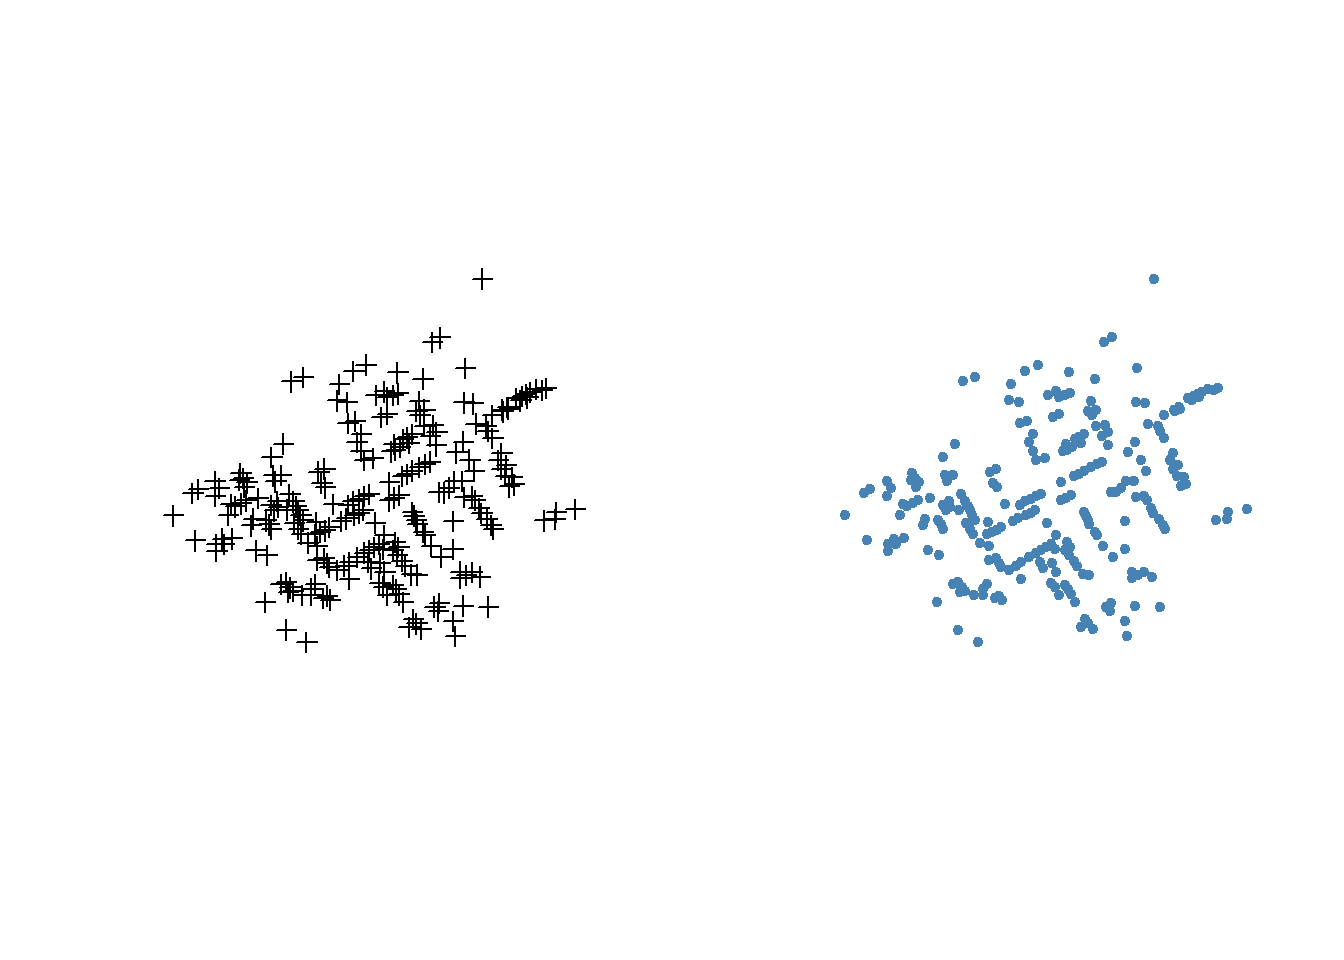
\includegraphics{modul_files/figure-latex/unnamed-chunk-9-1.pdf}

Perhatikan bahwa plot di atas hanya menunjukkan sebaran titik spasial, tanpa memberikan informasi yang jelas tentang lokasi data tersebut. Jika kita memiliki peta dalam bentuk data polygon, kita dapat mengimpor data tersebut dengan cara yang sama (seandainya datanya berupa shapefile), kemudian kita plot peta baru kemudian plot data titik seperti di atas.

Alternatif lainnya jika kita tidak ingin menggunakan peta polygon dari shapefile, kita dapat menggunakan beberapa package yang tersedia di R software, seperti \texttt{ggmap}, \texttt{OpenStreetMap}, \texttt{leaflet}, atau yang lain. Namun perhatikan bahwa untuk bisa menggunakan package \texttt{OpenStreetMap}, Anda harus memastikan bahwa jika Anda menggunakan \texttt{R} 64-bit maka \texttt{Java} yang terinstall di PC Anda juga harus sesuai, yaitu 64-bit.

Berikut ini akan ditunjukkan salah satu cara menampilkan peta dengan memanfaatkan package \texttt{leaflet}.

\begin{Shaded}
\begin{Highlighting}[]
\KeywordTok{library}\NormalTok{(leaflet)}
\NormalTok{map \textless{}{-}}\StringTok{ }\KeywordTok{leaflet}\NormalTok{() }\OperatorTok{\%\textgreater{}\%}\StringTok{ }\KeywordTok{setView}\NormalTok{(}\DataTypeTok{lng =}  \FloatTok{{-}0.13659}\NormalTok{, }\DataTypeTok{lat =}\FloatTok{51.51328}\NormalTok{ , }\DataTypeTok{zoom =} \DecValTok{12}\NormalTok{)}
\NormalTok{map }\OperatorTok{\%\textgreater{}\%}\StringTok{ }\KeywordTok{addTiles}\NormalTok{() }
\end{Highlighting}
\end{Shaded}

Sebelum kedua peta dan data titik digabungkan. Pastikan terlebih dahulu apakah koordinat yang digunakan menggunakan skala yang sama.

\begin{Shaded}
\begin{Highlighting}[]
\KeywordTok{head}\NormalTok{(}\KeywordTok{coordinates}\NormalTok{(CholeraDeaths))}
\end{Highlighting}
\end{Shaded}

\begin{verbatim}
##      coords.x1 coords.x2
## [1,]  529308.7  181031.4
## [2,]  529312.2  181025.2
## [3,]  529314.4  181020.3
## [4,]  529317.4  181014.3
## [5,]  529320.7  181007.9
## [6,]  529336.7  181006.0
\end{verbatim}

Seperti terlihat di atas, koordinat pada data \texttt{CholeraDeaths} diukur pada skala yang berbeda dengan peta yang diambil dari package \texttt{leaflet}. Terdapat beberapa macam \emph{coordinate reference system (CRS)}, beberapa di antaranya yang cukup populer adalah suatu set EPSG (\emph{European Petroleum Survey Group}) berikut:

\begin{itemize}
\item
  \textbf{EPSG:4326} juga dikenal sebagai WGS84, ukuran standard yang digunakan pada sistem GPS dan \emph{Google Earth}.
\item
  \textbf{EPSG:3857} digunakan pada Google Maps, Open Street Maps, dsb.
\item
  \textbf{EPSG:27700} juga dikenal sebagai OSGB 1936, atau \emph{British National Grid: United Kingdom Ordnance Survey}.
\end{itemize}

\begin{Shaded}
\begin{Highlighting}[]
\NormalTok{cholera\_latlong \textless{}{-}}\StringTok{ }\NormalTok{CholeraDeaths }\OperatorTok{\%\textgreater{}\%}\StringTok{ }
\StringTok{  }\KeywordTok{spTransform}\NormalTok{(}\KeywordTok{CRS}\NormalTok{(}\StringTok{"+init=epsg:4326"}\NormalTok{))}
\KeywordTok{leaflet}\NormalTok{(}\DataTypeTok{data =}\NormalTok{ CholeraDeaths) }\OperatorTok{\%\textgreater{}\%}\StringTok{ }
\StringTok{  }\KeywordTok{addTiles}\NormalTok{() }\OperatorTok{\%\textgreater{}\%}
\StringTok{  }\KeywordTok{addMarkers}\NormalTok{(cholera\_latlong}\OperatorTok{@}\NormalTok{coords[,}\DecValTok{1}\NormalTok{], cholera\_latlong}\OperatorTok{@}\NormalTok{coords[,}\DecValTok{2}\NormalTok{])}
\end{Highlighting}
\end{Shaded}

Dapat dilihat di atas, bahwa setelah koordinatnya disamakan, kita dapat menampilkan data \texttt{CholeraDeaths} pada peta yang diperoleh dari \texttt{Open\ Street\ Map} melalui package \texttt{leaflet}.

\hypertarget{tipe-data-spasial}{%
\section{Tipe Data Spasial}\label{tipe-data-spasial}}

\hypertarget{tipe-data-titik}{%
\subsection{Tipe Data titik}\label{tipe-data-titik}}

Data spasial dapat berupa titik pengamatan pada lokasi tertentu, yang umumnya menyimpan koordinat lokasi \emph{longitude} dan \emph{latitude}. Data jenis ini hanya memiliki nilai pada titik tertentu saja, misalnya data kejadian kecelakaan, data rumah sakit, data kejadian kriminal, dan lain-lain. Sebagai ilustrasi, akan diperlihatkan data atm dan SPBU berikut ini.

\begin{Shaded}
\begin{Highlighting}[]
\KeywordTok{library}\NormalTok{(rgdal)}
\NormalTok{petapontianak=}\KeywordTok{readOGR}\NormalTok{(}\DataTypeTok{dsn=}\StringTok{"Peta Pontianak"}\NormalTok{, }\DataTypeTok{layer=}\StringTok{"Pontianak\_kec"}\NormalTok{)}
\end{Highlighting}
\end{Shaded}

\begin{verbatim}
## OGR data source with driver: ESRI Shapefile 
## Source: "D:\Research (eksternal dept)\pelatihan spasial (adj)\modul\Peta Pontianak", layer: "Pontianak_kec"
## with 6 features
## It has 1 fields
\end{verbatim}

\begin{Shaded}
\begin{Highlighting}[]
\NormalTok{dataATM=}\KeywordTok{read.csv}\NormalTok{(}\StringTok{"DATA ATM PONTIANAK.csv"}\NormalTok{ , }\DataTypeTok{header=}\NormalTok{T)}
\NormalTok{dataSPBU=}\KeywordTok{read.csv}\NormalTok{(}\StringTok{"Data SPBU Pontianak.csv"}\NormalTok{, }\DataTypeTok{sep=}\StringTok{";"}\NormalTok{,}\DataTypeTok{header=}\NormalTok{T)}
\KeywordTok{plot}\NormalTok{(petapontianak)}
\KeywordTok{points}\NormalTok{(dataATM}\OperatorTok{$}\NormalTok{lon, dataATM}\OperatorTok{$}\NormalTok{lat, }\DataTypeTok{col=}\StringTok{"blue"}\NormalTok{, }\DataTypeTok{pch=}\DecValTok{3}\NormalTok{)}
\KeywordTok{points}\NormalTok{(dataSPBU}\OperatorTok{$}\NormalTok{lon, dataSPBU}\OperatorTok{$}\NormalTok{lat, }\DataTypeTok{col=}\StringTok{"red"}\NormalTok{, }\DataTypeTok{pch=}\DecValTok{3}\NormalTok{)}
\KeywordTok{title}\NormalTok{(}\StringTok{"Lokasi ATM dan SPBU di Pontianak"}\NormalTok{)}
\end{Highlighting}
\end{Shaded}

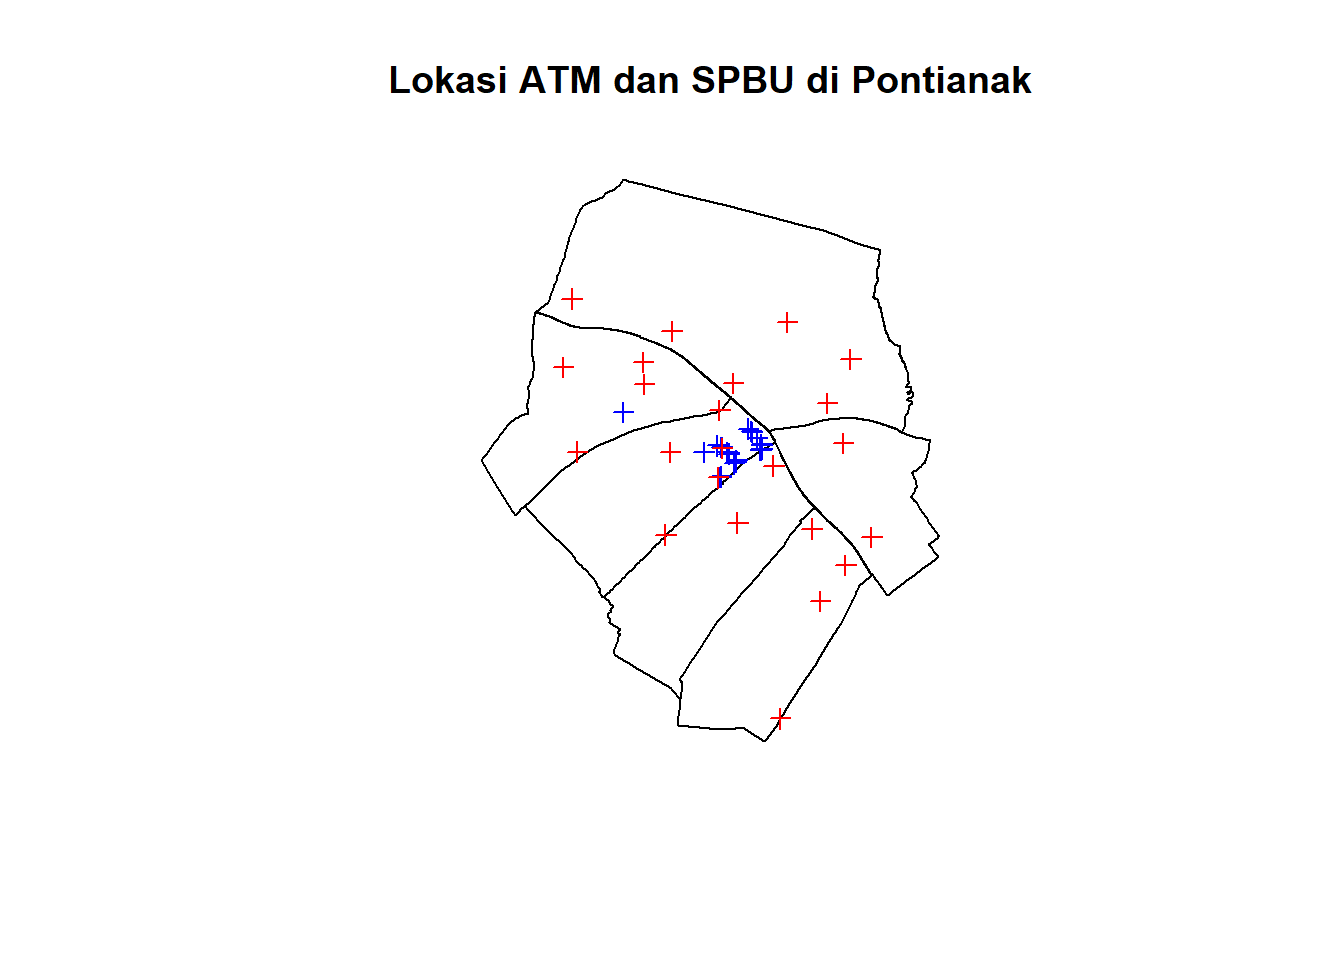
\includegraphics{modul_files/figure-latex/unnamed-chunk-13-1.pdf}

Data yang digunakan adalah berupa titik yang menunjukkan lokasi ATM dan SPBU. Lokasi ATM ditunjukkan dengan warna biru, sedangkan lokasi SPBU ditunjukkan dengan warna merah

\hypertarget{tipe-data-kontinu}{%
\subsection{Tipe Data Kontinu}\label{tipe-data-kontinu}}

Tipe data ini merupakan pengamatan yang memiliki nilai tidak hanya pada titik yang tersampel saja, namun nilai pengamatan sebenarnya kontinu untuk semua area. Artinya, di luar dari titik yang tersampel pun memiliki nilai untuk peubah yang diamati tersebut. Misalnya polusi udara, temperatur, kelembapan udara, presipitasi, dan sebagainya. Sebagai ilustrai, berikut ini adalah contoh data presipitasi di daerah Metro Manila.

\begin{Shaded}
\begin{Highlighting}[]
\KeywordTok{library}\NormalTok{(sp)}
\KeywordTok{library}\NormalTok{(gstat)}
\end{Highlighting}
\end{Shaded}

\begin{verbatim}
## Warning: package 'gstat' was built under R version 4.0.3
\end{verbatim}

\begin{Shaded}
\begin{Highlighting}[]
\NormalTok{metromanila=}\KeywordTok{read.csv}\NormalTok{(}\StringTok{"metromanila.csv"}\NormalTok{)}
\KeywordTok{coordinates}\NormalTok{(metromanila)\textless{}{-}}\KeywordTok{c}\NormalTok{(}\StringTok{"lon"}\NormalTok{,}\StringTok{"lat"}\NormalTok{)}
\KeywordTok{spplot}\NormalTok{(metromanila,}\StringTok{"precipitation"}\NormalTok{, }\DataTypeTok{asp =} \DecValTok{1}\NormalTok{,}
       \DataTypeTok{cex=}\FloatTok{0.5}\NormalTok{, }\DataTypeTok{pch =} \DecValTok{19}\NormalTok{, }\DataTypeTok{main=}\StringTok{"Angka Presipitasi di Metro Manila"}\NormalTok{)}
\end{Highlighting}
\end{Shaded}

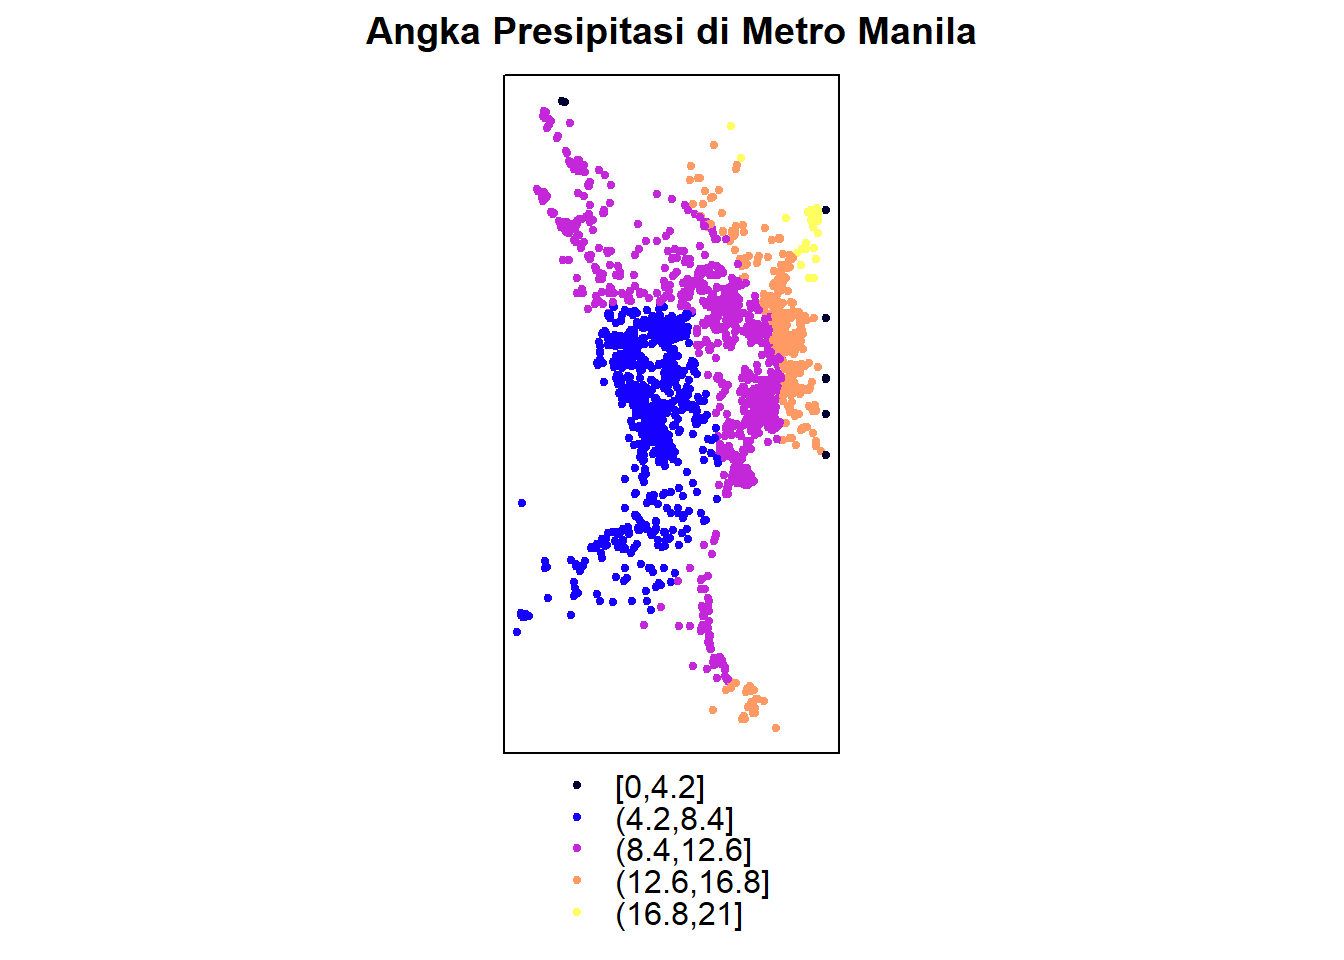
\includegraphics{modul_files/figure-latex/unnamed-chunk-14-1.pdf}

\hypertarget{tipe-data-area}{%
\subsection{Tipe Data Area}\label{tipe-data-area}}

Pada tipe data ini, pengamatan dilakukan pada level area. Area dapat mengacu pada sistem administrasi misalnya desa, kelurahan, kecamatan, kota, bahkan negara. Berikut ini adalah contoh data area yang diukur pada level kabupaten/kota. Untuk selanjutnya, pengamatan pada berbagai peubah dapat ditambahkan ke dalam data agar dapat diolah pada tahap analisis berikutnya.

\begin{Shaded}
\begin{Highlighting}[]
\KeywordTok{library}\NormalTok{(spdep)}
\KeywordTok{library}\NormalTok{(rgdal)}
\KeywordTok{library}\NormalTok{(raster)}
\NormalTok{petajawa\textless{}{-}}\StringTok{ }\KeywordTok{readOGR}\NormalTok{(}\DataTypeTok{dsn =} \StringTok{"Jawamap"}\NormalTok{, }\DataTypeTok{layer=}\StringTok{"jawa"}\NormalTok{)}
\end{Highlighting}
\end{Shaded}

\begin{verbatim}
## OGR data source with driver: ESRI Shapefile 
## Source: "D:\Research (eksternal dept)\pelatihan spasial (adj)\modul\Jawamap", layer: "jawa"
## with 119 features
## It has 5 fields
\end{verbatim}

\begin{Shaded}
\begin{Highlighting}[]
\KeywordTok{plot}\NormalTok{(petajawa)}
\end{Highlighting}
\end{Shaded}

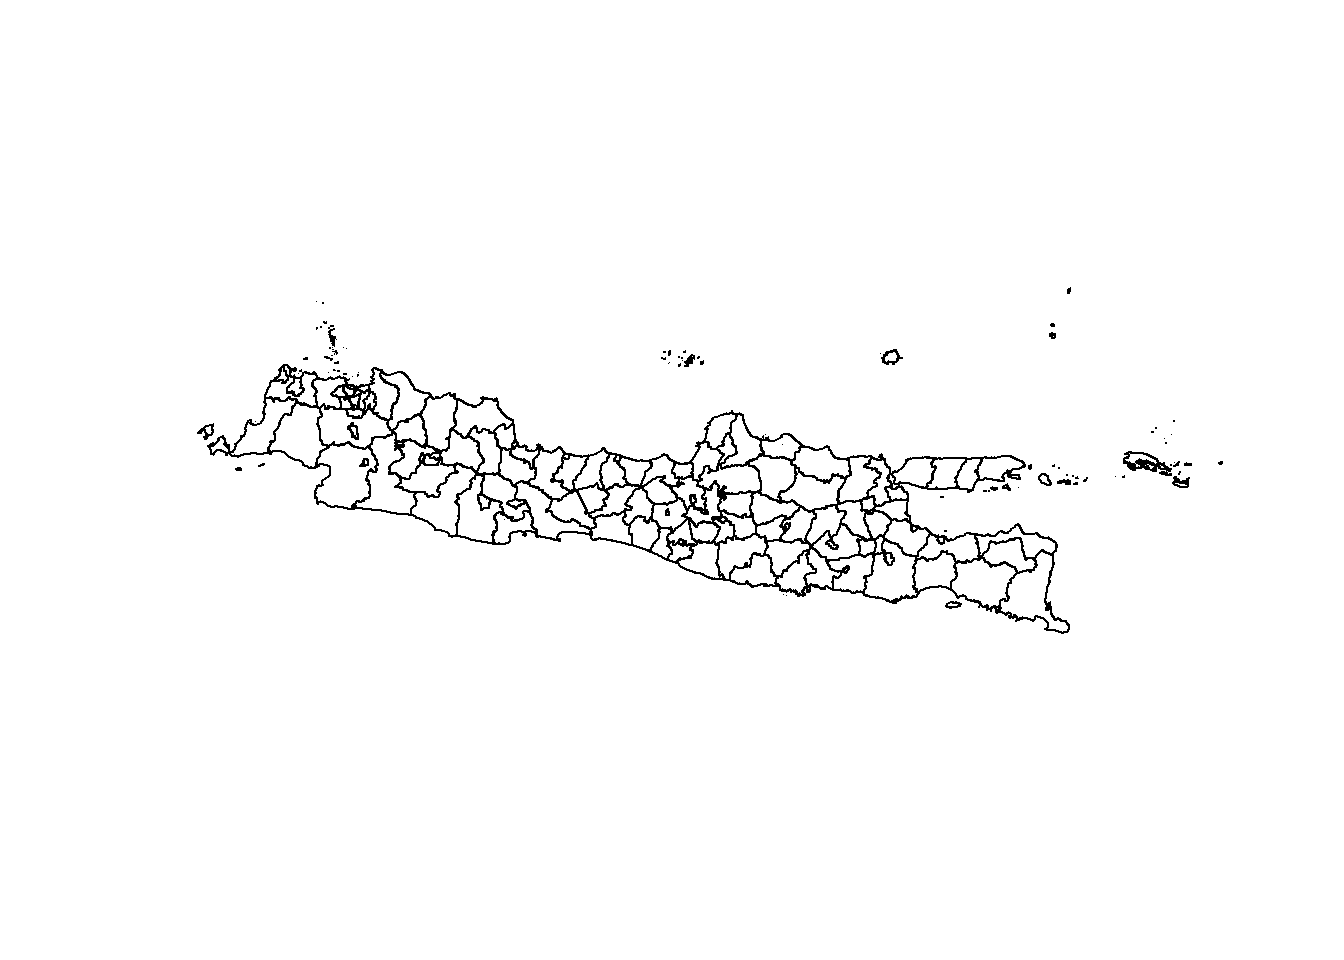
\includegraphics{modul_files/figure-latex/unnamed-chunk-15-1.pdf}

\hypertarget{matriks-bobot-dan-autokorelasi-spasial}{%
\section{Matriks Bobot dan Autokorelasi Spasial}\label{matriks-bobot-dan-autokorelasi-spasial}}

Pada analisis data spasial, informasi ketergantungan antar lokasi dapat diukur dengan autokorelasi spasial. Untuk dapat menghitung nilai autokorelasi tersebut, terdapat beberapa tahap yang perlu dilakukan, yaitu:

\begin{enumerate}
\def\labelenumi{(\arabic{enumi})}
\item
  menentukan kriteria kebertentanggaan antar lokasi pengamatan
\item
  menyusun matriks bobot spasial
\item
  matriks bobot spasial selanjutnya dapat dimanfaatkan baik untuk mengukur autokorelasi spasial maupun untuk menyusun pemodelan spasial.
\end{enumerate}

\hypertarget{kriteria-kebertetanggaan}{%
\subsection{Kriteria Kebertetanggaan}\label{kriteria-kebertetanggaan}}

Ilustrasi yang akan digunakan pada bagian ini adalah data yang tersedia di dalam R. Data tersebut dapat dipanggil dengan fungsi berikut.

\begin{Shaded}
\begin{Highlighting}[]
\KeywordTok{library}\NormalTok{(raster)}
\NormalTok{p \textless{}{-}}\StringTok{ }\KeywordTok{shapefile}\NormalTok{(}\KeywordTok{system.file}\NormalTok{(}\StringTok{"external/lux.shp"}\NormalTok{, }\DataTypeTok{package=}\StringTok{"raster"}\NormalTok{))}
\NormalTok{p \textless{}{-}}\StringTok{ }\NormalTok{p[p}\OperatorTok{$}\NormalTok{NAME\_}\DecValTok{1}\OperatorTok{==}\StringTok{"Diekirch"}\NormalTok{, ]}
\end{Highlighting}
\end{Shaded}

Selanjutnya kita akan tentukan sembarang nilai yang akan disimpan pada setiap lokasi untuk mengilustrasikan nilai peubah yang diamati.

\begin{Shaded}
\begin{Highlighting}[]
\NormalTok{p}\OperatorTok{$}\NormalTok{value \textless{}{-}}\StringTok{ }\KeywordTok{c}\NormalTok{(}\DecValTok{10}\NormalTok{, }\DecValTok{6}\NormalTok{, }\DecValTok{4}\NormalTok{, }\DecValTok{11}\NormalTok{, }\DecValTok{6}\NormalTok{)}
\KeywordTok{data.frame}\NormalTok{(p)}
\end{Highlighting}
\end{Shaded}

\begin{verbatim}
##   ID_1   NAME_1 ID_2   NAME_2 AREA value
## 0    1 Diekirch    1 Clervaux  312    10
## 1    1 Diekirch    2 Diekirch  218     6
## 2    1 Diekirch    3  Redange  259     4
## 3    1 Diekirch    4  Vianden   76    11
## 4    1 Diekirch    5    Wiltz  263     6
\end{verbatim}

Berikut adalah visualisasi dari data yang telah kita persiapkan.

\begin{Shaded}
\begin{Highlighting}[]
\KeywordTok{par}\NormalTok{(}\DataTypeTok{mai=}\KeywordTok{c}\NormalTok{(}\DecValTok{0}\NormalTok{,}\DecValTok{0}\NormalTok{,}\DecValTok{0}\NormalTok{,}\DecValTok{0}\NormalTok{))}
\KeywordTok{plot}\NormalTok{(p, }\DataTypeTok{col=}\DecValTok{2}\OperatorTok{:}\DecValTok{7}\NormalTok{)}
\NormalTok{coords \textless{}{-}}\StringTok{ }\KeywordTok{coordinates}\NormalTok{(p)}
\KeywordTok{points}\NormalTok{(coords, }\DataTypeTok{cex=}\DecValTok{6}\NormalTok{, }\DataTypeTok{pch=}\DecValTok{20}\NormalTok{, }\DataTypeTok{col=}\StringTok{\textquotesingle{}white\textquotesingle{}}\NormalTok{)}
\KeywordTok{text}\NormalTok{(p, }\StringTok{\textquotesingle{}ID\_2\textquotesingle{}}\NormalTok{, }\DataTypeTok{cex=}\FloatTok{1.5}\NormalTok{)}
\end{Highlighting}
\end{Shaded}

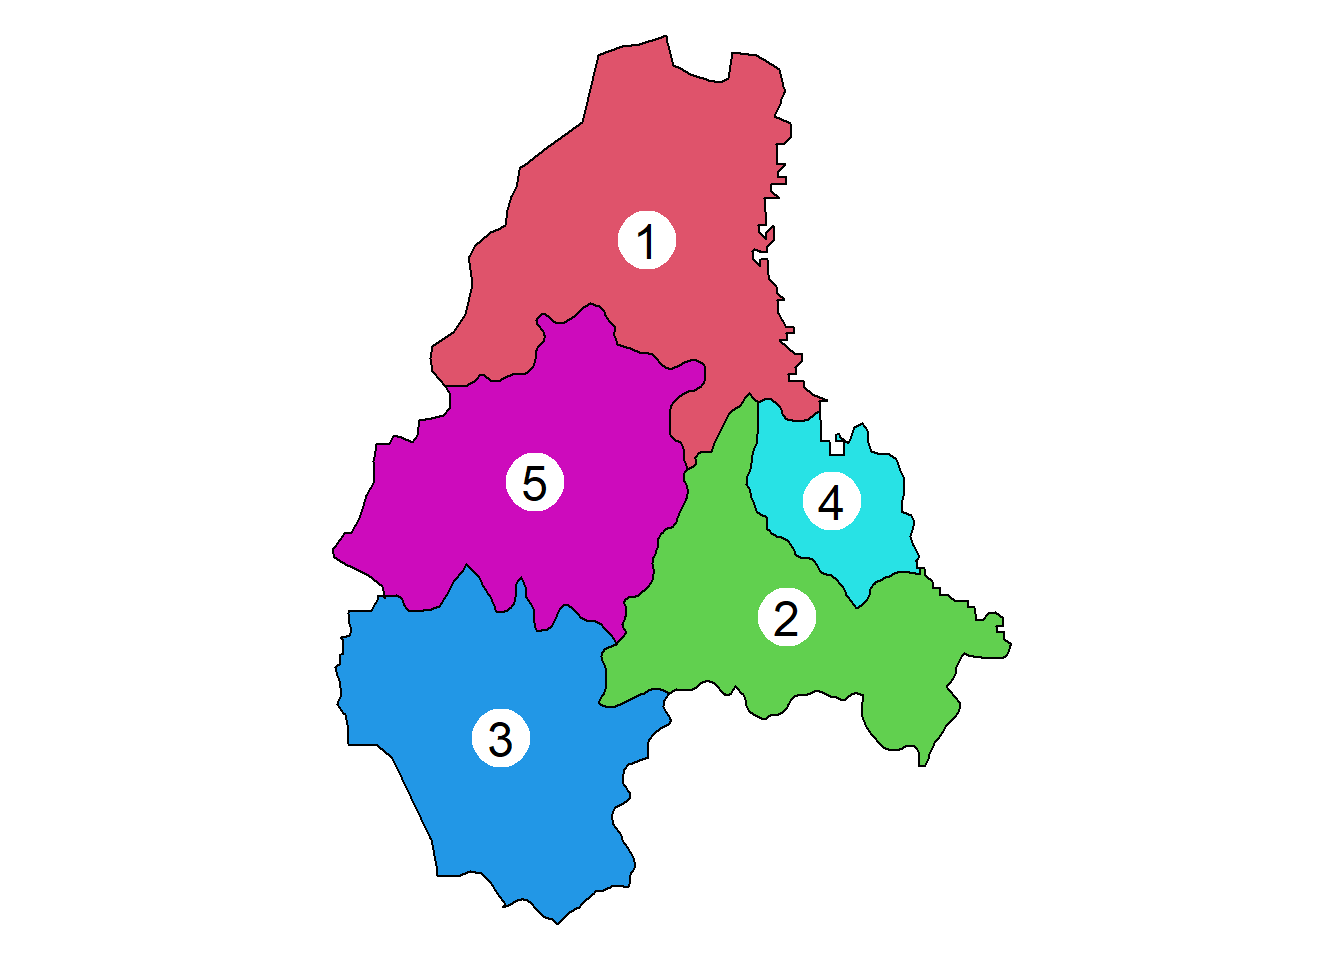
\includegraphics{modul_files/figure-latex/unnamed-chunk-18-1.pdf}

\hypertarget{contiguity-based}{%
\subsubsection{\texorpdfstring{\emph{Contiguity Based}}{Contiguity Based}}\label{contiguity-based}}

Kriteria yang umum digunakan pada ketetanggaan berbasis \emph{contiguity} adalah \emph{queen contiguity}, \emph{rook contiguity}, dan \emph{bishop contiguity}, seperti yang terlihat pada ilustrasi berikut ini.

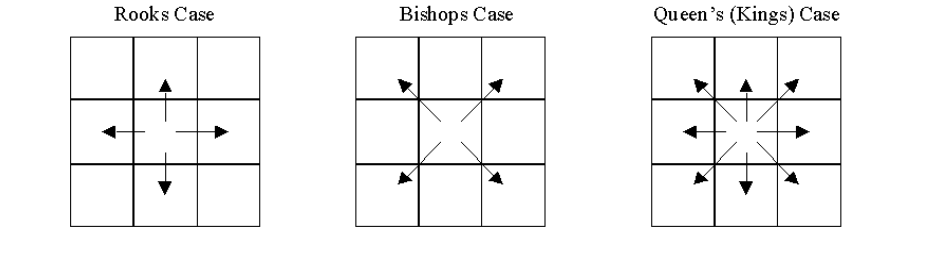
\includegraphics{D:/Research (eksternal dept)/pelatihan spasial (adj)/Modul Pelatihan Spasial/gambar 1.png}

Program berikut ini dapat diguakan untuk dapat memperoleh matriks bobot berdasarkan kriteria \emph{queen contiguity}.

\begin{Shaded}
\begin{Highlighting}[]
\KeywordTok{library}\NormalTok{(spdep)}
\NormalTok{w \textless{}{-}}\StringTok{ }\KeywordTok{poly2nb}\NormalTok{(p)}

\CommentTok{\#lebih lengkap dapat dituliskan seperti berikut ini:}
\NormalTok{w \textless{}{-}}\StringTok{ }\KeywordTok{poly2nb}\NormalTok{(p, }\DataTypeTok{queen=}\OtherTok{TRUE}\NormalTok{)}

\KeywordTok{plot}\NormalTok{(p)}
\KeywordTok{plot}\NormalTok{(w, coords, }\DataTypeTok{add=}\NormalTok{T)}
\end{Highlighting}
\end{Shaded}

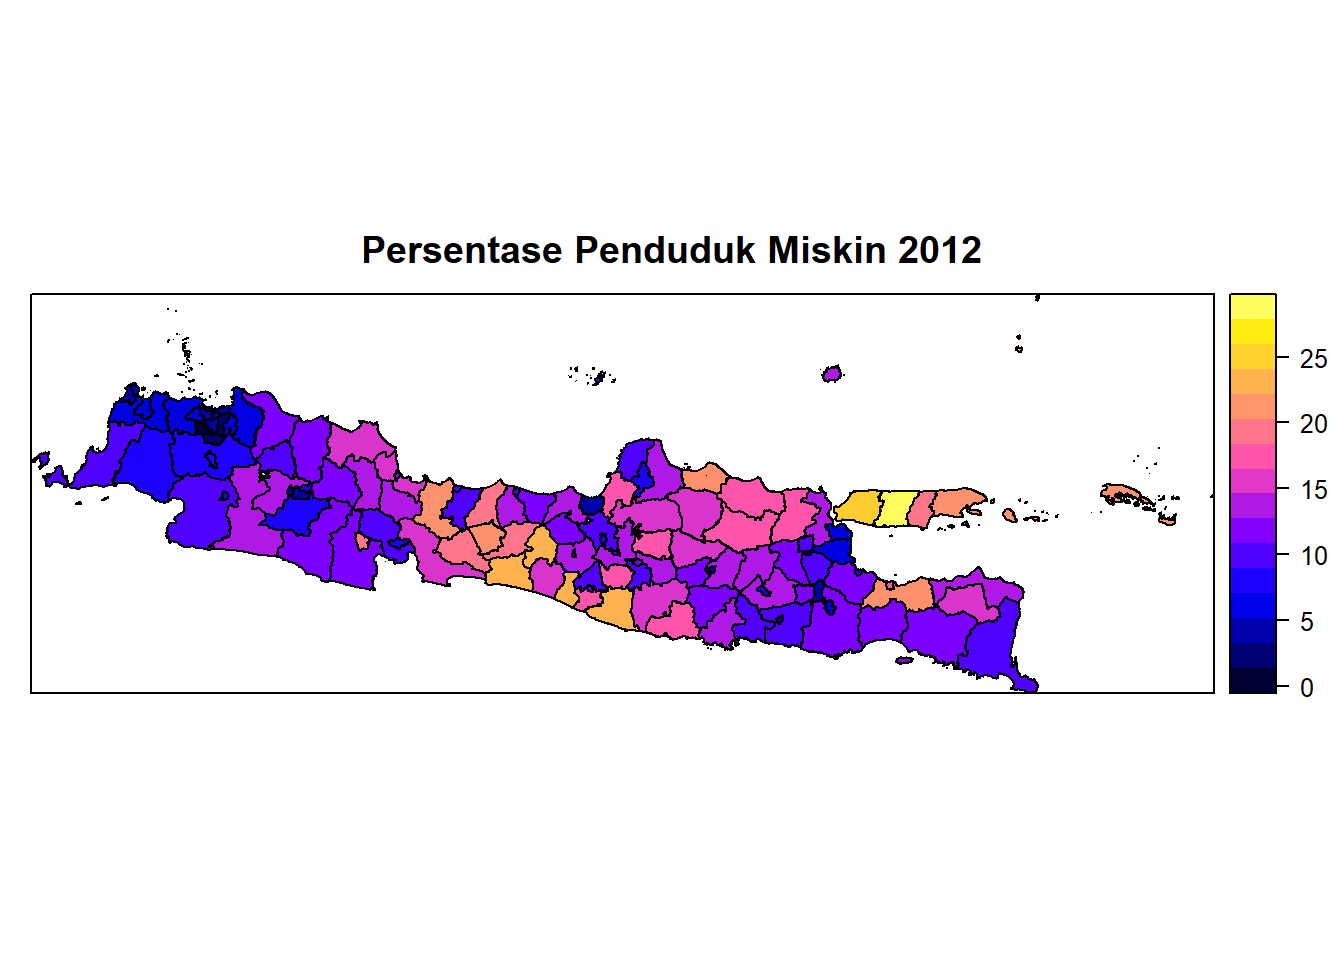
\includegraphics{modul_files/figure-latex/unnamed-chunk-19-1.pdf}

Jika yang ingin digunakan adalah kriteria \emph{rook contiguity}, maka kita dapat mengganti argumen pada program sebelumnya menjadi \texttt{queen=FALSE}.

\begin{Shaded}
\begin{Highlighting}[]
\NormalTok{w.rook \textless{}{-}}\StringTok{ }\KeywordTok{poly2nb}\NormalTok{(p, }\DataTypeTok{queen=}\OtherTok{FALSE}\NormalTok{)}
\NormalTok{coords\textless{}{-}}\KeywordTok{coordinates}\NormalTok{(p)}
\KeywordTok{plot}\NormalTok{(p)}
\KeywordTok{plot}\NormalTok{(w, coords, }\DataTypeTok{add=}\NormalTok{T)}
\end{Highlighting}
\end{Shaded}

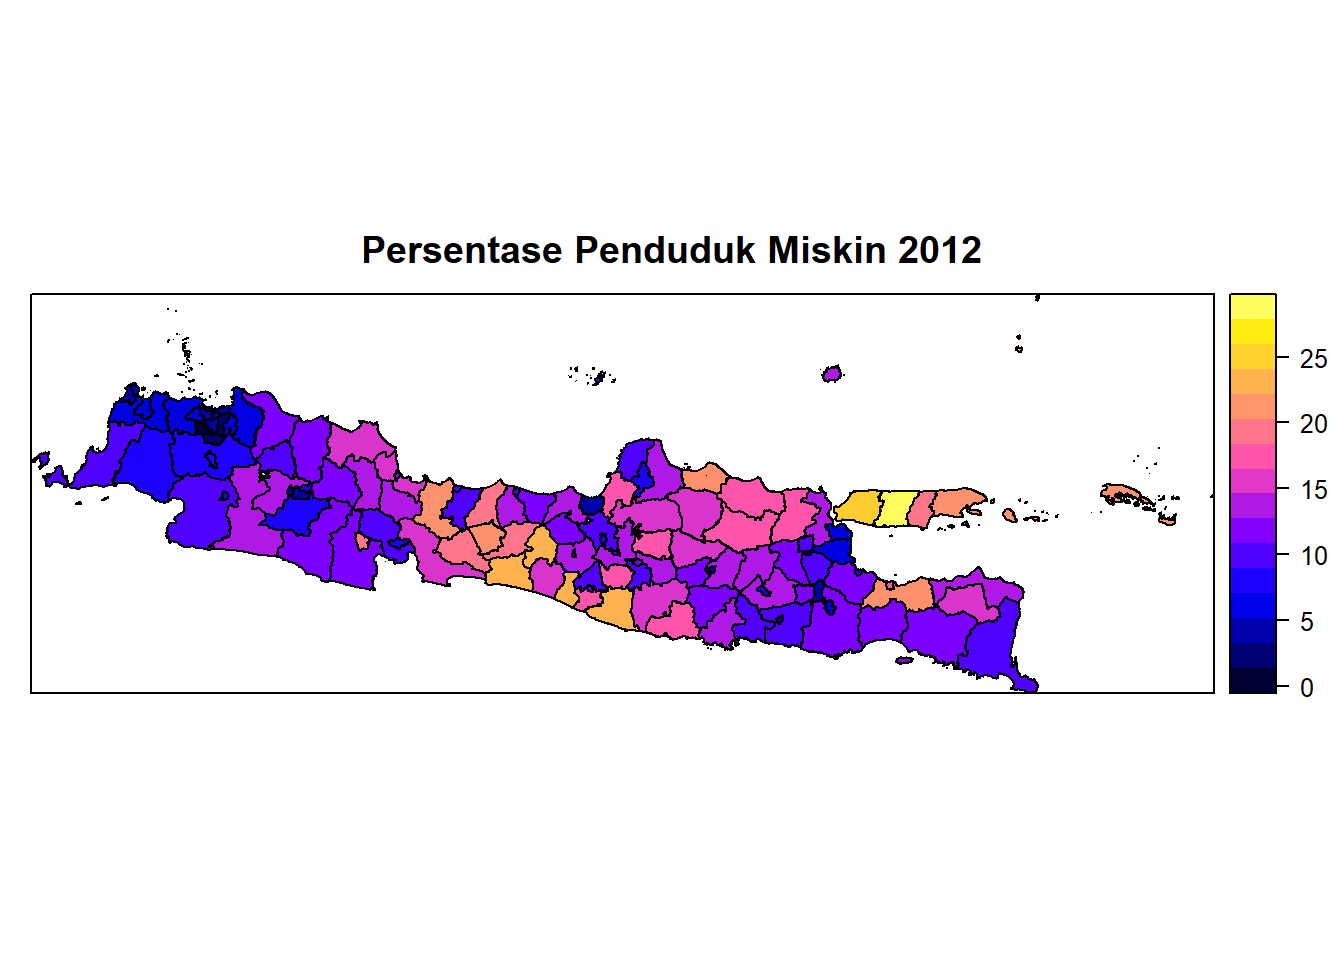
\includegraphics{modul_files/figure-latex/unnamed-chunk-20-1.pdf}

Perhatikan bahwa pada kasus ini, kedua kriteria memperlihatkan hasil yang sama. Hal ini terjadi karena semua area pada ilustrasi ini bersinggungan sudut.

\hypertarget{distance-based}{%
\subsubsection{\texorpdfstring{\emph{Distance Based}}{Distance Based}}\label{distance-based}}

Kriteria kebertetanggaan dapat pula ditentukan berdasarkan jarak antar lokasi, beberapa pendekatan jarak yang dapat digunakan adalah \(k\) tetangga terdekat (\emph{k nearest neighbours (KNN)}), \emph{radial distance}, \emph{power distance}, dan \emph{exponential distance}. Ilustrasi KNN dan \emph{radial distance} dapat dilihat pada subbab berikutnya dalam modul ini.

Pendekatan \emph{power distance} dan \emph{exponential distance} tidak diberikan ilustrasi pada modul ini, namun berikut adalah penjelasan singkat mengenai keduanya. Apabila bobot antara lokasi ke-\(i\) dan lokasi ke-\(j\) dinotasikan dengan \(w_{ij}\), dan jarak antara kedua lokasi tersebut dinotasikan dengan \(d_{ij}\), formula untuk memperoleh bobot jarak dengan pendekatan \emph{power distance} adalah:
\[
w_{ij}=d_{ij}^{-\alpha}
\]

Sedangkan bobot jarak berdasarkan \emph{exponential distance} dapat diperoleh dengan formula:
\[
w_{ij}=e^{{-\alpha}d_{ij}}
\]

\hypertarget{k-nearest-neighbours}{%
\paragraph{\texorpdfstring{\emph{K-Nearest Neighbours}}{K-Nearest Neighbours}}\label{k-nearest-neighbours}}

Pada pendekatan ini, kita mendefinisikan lokasi yang merupakan tetangga dari lokasi ke-\(i\) adalah sejumlah \(k\) lokasi yang memiliki jarak terdekat dengan lokasi \(i\).

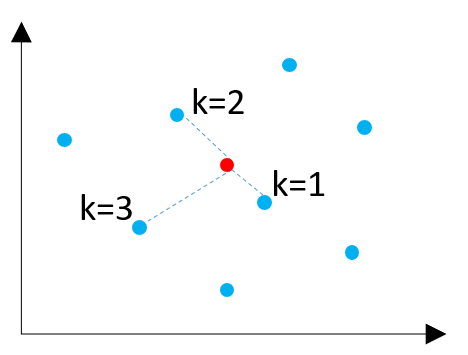
\includegraphics{D:/Research (eksternal dept)/pelatihan spasial (adj)/Modul Pelatihan Spasial/knn.png}

Berikut ini adalah ilustrasi untuk memperoleh ketetanggaan dengan pendekatan KNN menggunakan program R.

\begin{Shaded}
\begin{Highlighting}[]
\NormalTok{coords\textless{}{-}}\KeywordTok{coordinates}\NormalTok{(p)}
\NormalTok{IDs\textless{}{-}}\KeywordTok{row.names}\NormalTok{(}\KeywordTok{as}\NormalTok{(p, }\StringTok{"data.frame"}\NormalTok{))}
\NormalTok{p\_kn1\textless{}{-}}\KeywordTok{knn2nb}\NormalTok{(}\KeywordTok{knearneigh}\NormalTok{(coords, }\DataTypeTok{k=}\DecValTok{1}\NormalTok{), }\DataTypeTok{row.names=}\NormalTok{IDs)}
\NormalTok{p\_kn2\textless{}{-}}\KeywordTok{knn2nb}\NormalTok{(}\KeywordTok{knearneigh}\NormalTok{(coords, }\DataTypeTok{k=}\DecValTok{2}\NormalTok{), }\DataTypeTok{row.names=}\NormalTok{IDs)}
\NormalTok{p\_kn4\textless{}{-}}\KeywordTok{knn2nb}\NormalTok{(}\KeywordTok{knearneigh}\NormalTok{(coords, }\DataTypeTok{k=}\DecValTok{4}\NormalTok{), }\DataTypeTok{row.names=}\NormalTok{IDs)}

\KeywordTok{par}\NormalTok{(}\DataTypeTok{mfrow=}\KeywordTok{c}\NormalTok{(}\DecValTok{1}\NormalTok{,}\DecValTok{3}\NormalTok{))}
\KeywordTok{plot}\NormalTok{(p, }\DataTypeTok{main =} \StringTok{"k=1"}\NormalTok{)}
\KeywordTok{plot}\NormalTok{(p\_kn1, coords, }\DataTypeTok{add=}\NormalTok{T)}

\KeywordTok{plot}\NormalTok{(p, }\DataTypeTok{main =} \StringTok{"k=2"}\NormalTok{)}
\KeywordTok{plot}\NormalTok{(p\_kn2, coords, }\DataTypeTok{add=}\NormalTok{T)}

\KeywordTok{plot}\NormalTok{(p, }\DataTypeTok{main =} \StringTok{"k=4"}\NormalTok{)}
\KeywordTok{plot}\NormalTok{(p\_kn4, coords, }\DataTypeTok{add=}\NormalTok{T)}
\end{Highlighting}
\end{Shaded}

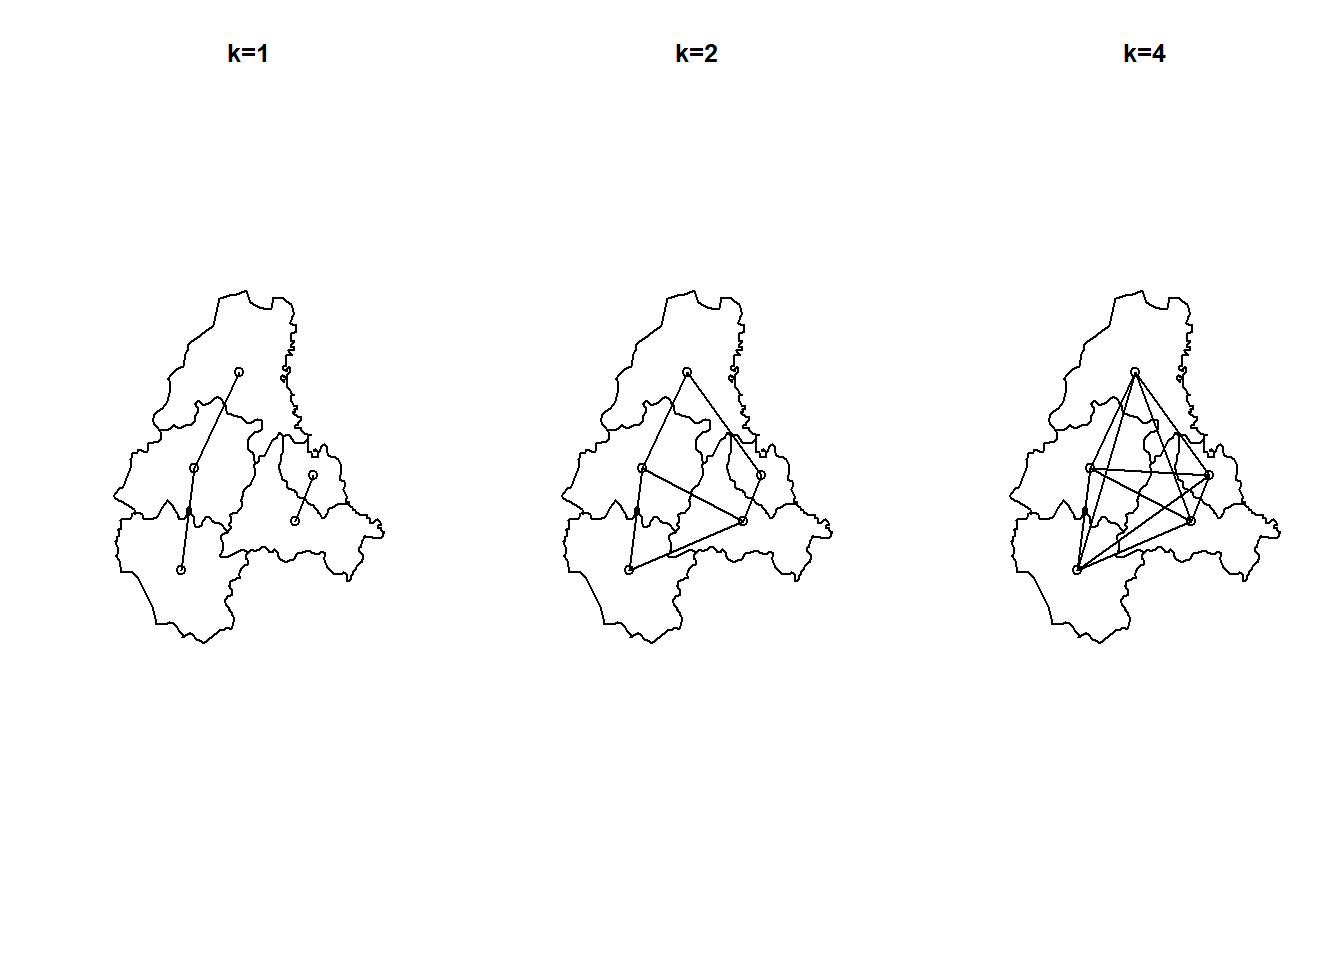
\includegraphics{modul_files/figure-latex/unnamed-chunk-21-1.pdf}

\hypertarget{radial-distance}{%
\paragraph{\texorpdfstring{\emph{Radial Distance}}{Radial Distance}}\label{radial-distance}}

Pada pendekatan ini,kita mendefinisikan lokasi yang merupakan tetangga dari lokasi ke-\(i\) adalah sejumlah \(k\) lokasi yang berada batas batas jarak (radius) antara \(d1\) dan \(d2\), diukur dari lokasi \(i\).

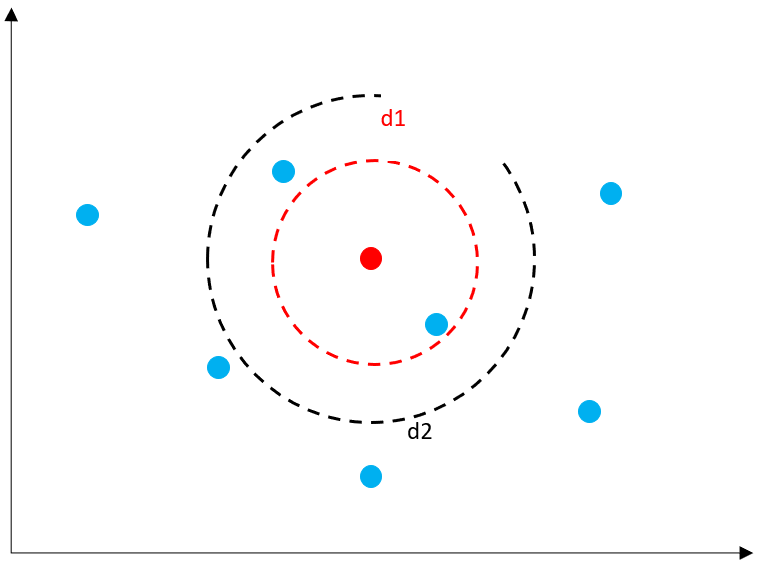
\includegraphics{D:/Research (eksternal dept)/pelatihan spasial (adj)/Modul Pelatihan Spasial/radial_distance.png}

Berikut ini adalah ilustrasi untuk memperoleh ketetanggaan dengan pendekatan KNN menggunakan program R.

\begin{Shaded}
\begin{Highlighting}[]
\NormalTok{dist\textless{}{-}}\KeywordTok{unlist}\NormalTok{(}\KeywordTok{nbdists}\NormalTok{(p\_kn1, coords))}
\KeywordTok{summary}\NormalTok{(dist)}
\end{Highlighting}
\end{Shaded}

\begin{verbatim}
##    Min. 1st Qu.  Median    Mean 3rd Qu.    Max. 
## 0.07316 0.07316 0.14159 0.11832 0.14159 0.16213
\end{verbatim}

\begin{Shaded}
\begin{Highlighting}[]
\KeywordTok{sort}\NormalTok{(dist)}
\end{Highlighting}
\end{Shaded}

\begin{verbatim}
## [1] 0.07315711 0.07315711 0.14158521 0.14158521 0.16213194
\end{verbatim}

\begin{Shaded}
\begin{Highlighting}[]
\NormalTok{max\_k1\textless{}{-}}\KeywordTok{max}\NormalTok{(dist)}
\NormalTok{p\_kd1\textless{}{-}}\KeywordTok{dnearneigh}\NormalTok{(coords, }\DataTypeTok{d1=}\DecValTok{0}\NormalTok{, }\DataTypeTok{d2=}\FloatTok{0.75}\OperatorTok{*}\NormalTok{max\_k1, }\DataTypeTok{row.names=}\NormalTok{IDs)}
\NormalTok{p\_kd2\textless{}{-}}\KeywordTok{dnearneigh}\NormalTok{(coords, }\DataTypeTok{d1=}\DecValTok{0}\NormalTok{, }\DataTypeTok{d2=}\DecValTok{1}\OperatorTok{*}\NormalTok{max\_k1, }\DataTypeTok{row.names=}\NormalTok{IDs)}
\NormalTok{p\_kd3\textless{}{-}}\KeywordTok{dnearneigh}\NormalTok{(coords, }\DataTypeTok{d1=}\DecValTok{0}\NormalTok{, }\DataTypeTok{d2=}\FloatTok{1.5}\OperatorTok{*}\NormalTok{max\_k1, }\DataTypeTok{row.names=}\NormalTok{IDs)}

\KeywordTok{par}\NormalTok{(}\DataTypeTok{mfrow=}\KeywordTok{c}\NormalTok{(}\DecValTok{1}\NormalTok{,}\DecValTok{3}\NormalTok{))}
\KeywordTok{plot}\NormalTok{(p, }\DataTypeTok{main =} \StringTok{"Distance=0.75*max\_k1"}\NormalTok{)}
\KeywordTok{plot}\NormalTok{(p\_kd1,coords, }\DataTypeTok{add=}\NormalTok{T)}

\KeywordTok{plot}\NormalTok{(p, }\DataTypeTok{main =} \StringTok{"Distance=1*max\_k1"}\NormalTok{)}
\KeywordTok{plot}\NormalTok{(p\_kd2,coords, }\DataTypeTok{add=}\NormalTok{T)}

\KeywordTok{plot}\NormalTok{(p, }\DataTypeTok{main =} \StringTok{"Distance=1.5*max\_k1"}\NormalTok{)}
\KeywordTok{plot}\NormalTok{(p\_kd3,coords, }\DataTypeTok{add=}\NormalTok{T)}
\end{Highlighting}
\end{Shaded}

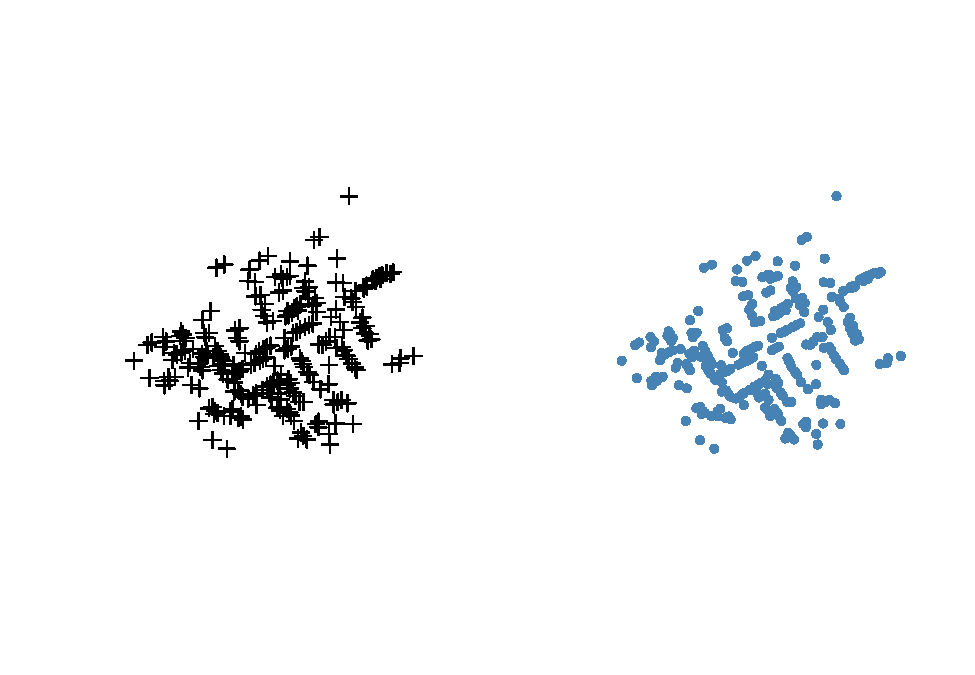
\includegraphics{modul_files/figure-latex/unnamed-chunk-22-1.pdf}

\hypertarget{matriks-pembobot-spasial}{%
\subsection{Matriks Pembobot Spasial}\label{matriks-pembobot-spasial}}

Matriks pembobot spasial dapat berisi elemen biner (1 atau 0) untuk menunjukkan ketetanggaan setiap lokasi, atau berupa matriks yang sudah distandardisasi. Umumnya, matriks pembobot spasial merupakan matriks yang terstandardisasi baris (\emph{row standardized}).

\begin{Shaded}
\begin{Highlighting}[]
\KeywordTok{nb2mat}\NormalTok{(w, }\DataTypeTok{style=}\StringTok{"B"}\NormalTok{)  }\CommentTok{\#matriks pembobot biner}
\end{Highlighting}
\end{Shaded}

\begin{verbatim}
##   [,1] [,2] [,3] [,4] [,5]
## 0    0    1    0    1    1
## 1    1    0    1    1    1
## 2    0    1    0    0    1
## 3    1    1    0    0    0
## 4    1    1    1    0    0
## attr(,"call")
## nb2mat(neighbours = w, style = "B")
\end{verbatim}

\begin{Shaded}
\begin{Highlighting}[]
\KeywordTok{nb2mat}\NormalTok{(w) }\CommentTok{\# matriks pembobot row standardized}
\end{Highlighting}
\end{Shaded}

\begin{verbatim}
##        [,1]      [,2]      [,3]      [,4]      [,5]
## 0 0.0000000 0.3333333 0.0000000 0.3333333 0.3333333
## 1 0.2500000 0.0000000 0.2500000 0.2500000 0.2500000
## 2 0.0000000 0.5000000 0.0000000 0.0000000 0.5000000
## 3 0.5000000 0.5000000 0.0000000 0.0000000 0.0000000
## 4 0.3333333 0.3333333 0.3333333 0.0000000 0.0000000
## attr(,"call")
## nb2mat(neighbours = w)
\end{verbatim}

\hypertarget{autokorelasi-spasial}{%
\subsection{Autokorelasi Spasial}\label{autokorelasi-spasial}}

\hypertarget{indeks-moran-global}{%
\subsubsection{Indeks Moran Global}\label{indeks-moran-global}}

Sebagai ilustrasi, akan digunakan data persentase kemiskinan kabupaten/kota di Pulau Jawa. Berikut adalah syntax untuk membaca peta Pulau Jawa dan data persentase kemiskinan Kabupaten/Kota di Pulau Jawa

\begin{Shaded}
\begin{Highlighting}[]
\KeywordTok{library}\NormalTok{(rgdal)}
\KeywordTok{library}\NormalTok{(spdep)}
\KeywordTok{library}\NormalTok{(sp)}
\NormalTok{petajawa=}\KeywordTok{readOGR}\NormalTok{(}\DataTypeTok{dsn=}\StringTok{"Jawamap"}\NormalTok{, }\DataTypeTok{layer=}\StringTok{"jawa"}\NormalTok{)}
\end{Highlighting}
\end{Shaded}

\begin{verbatim}
## OGR data source with driver: ESRI Shapefile 
## Source: "D:\Research (eksternal dept)\pelatihan spasial (adj)\modul\Jawamap", layer: "jawa"
## with 119 features
## It has 5 fields
\end{verbatim}

\begin{Shaded}
\begin{Highlighting}[]
\NormalTok{datajawa=}\KeywordTok{read.csv}\NormalTok{(}\StringTok{"Pulau Jawa.csv"}\NormalTok{, }\DataTypeTok{header=}\NormalTok{T, }\DataTypeTok{sep=}\StringTok{";"}\NormalTok{)}
\NormalTok{petajawa}\OperatorTok{$}\NormalTok{Kemiskinan\textless{}{-}}\StringTok{ }\NormalTok{datajawa}\OperatorTok{$}\NormalTok{Kemiskinan}
\NormalTok{k=}\DecValTok{9}
\NormalTok{colfunc \textless{}{-}}\StringTok{ }\KeywordTok{colorRampPalette}\NormalTok{(}\KeywordTok{c}\NormalTok{(}\StringTok{"green"}\NormalTok{, }\StringTok{"yellow"}\NormalTok{,}\StringTok{"red"}\NormalTok{))}
\NormalTok{color \textless{}{-}}\StringTok{ }\KeywordTok{colfunc}\NormalTok{(k)}
\KeywordTok{spplot}\NormalTok{(petajawa, }\StringTok{"Kemiskinan"}\NormalTok{, }\DataTypeTok{col.regions=}\NormalTok{color)}
\end{Highlighting}
\end{Shaded}

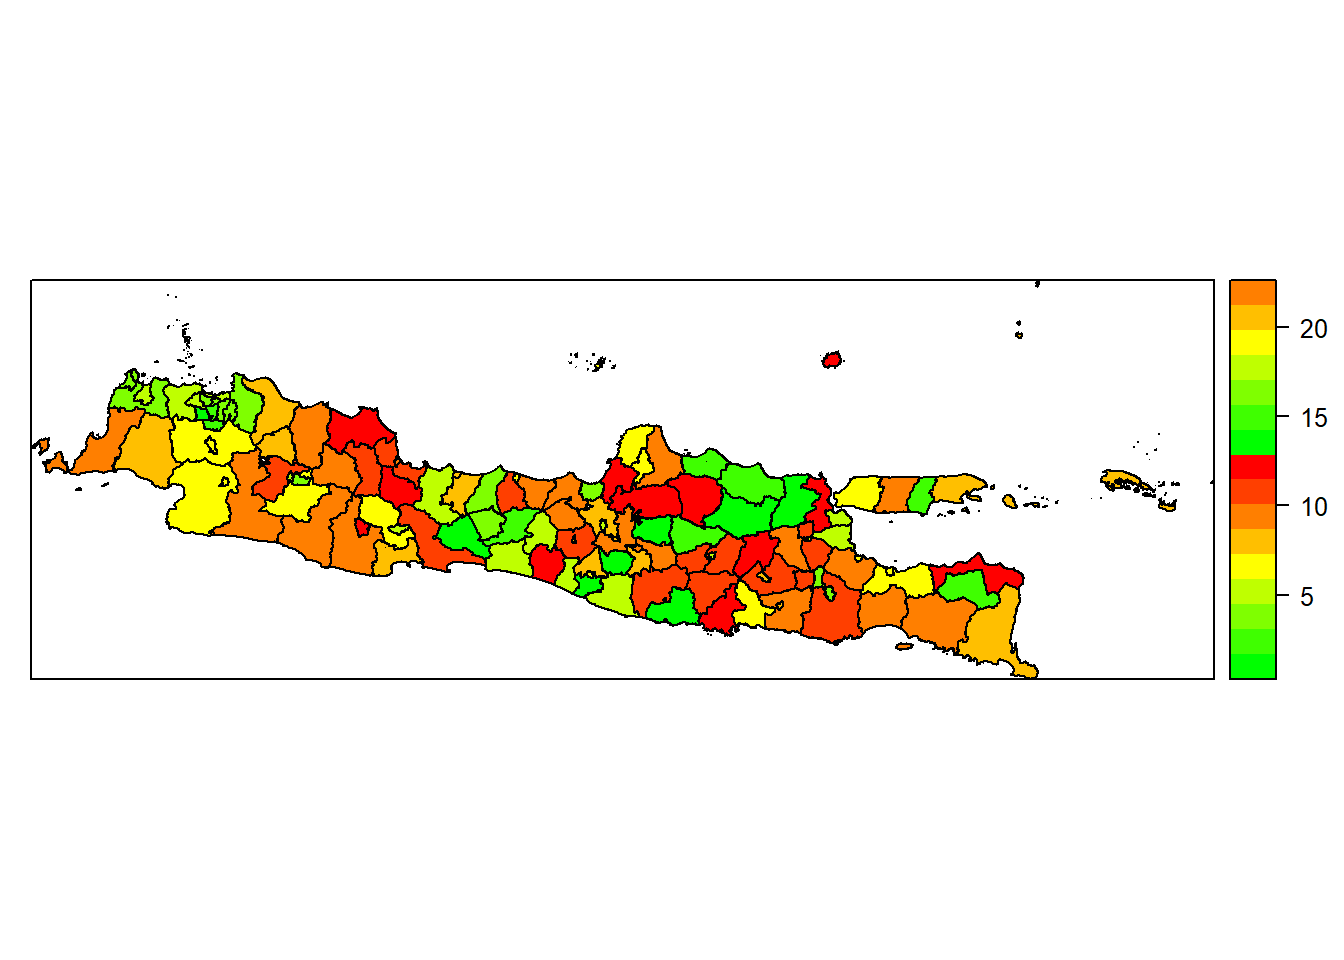
\includegraphics{modul_files/figure-latex/unnamed-chunk-25-1.pdf}

Seandainya kita akan menggunakan kriteria queen contiguity, maka dapat dilakukan dengan syntax berikut untuk mendefinisikan matriks pembobotnya

\begin{Shaded}
\begin{Highlighting}[]
\NormalTok{w.queen \textless{}{-}}\StringTok{ }\KeywordTok{poly2nb}\NormalTok{(petajawa)}
\NormalTok{w.queen}
\end{Highlighting}
\end{Shaded}

\begin{verbatim}
## Neighbour list object:
## Number of regions: 119 
## Number of nonzero links: 522 
## Percentage nonzero weights: 3.68618 
## Average number of links: 4.386555 
## 1 region with no links:
## 0
\end{verbatim}

Terlihat pada output tersebut, bahwa terdapat 1 wilayah yang tidak memiliki tetangga, sehingga untuk syntax selanjutnya perlu ditambahkan \texttt{zero.policy=T}.

\begin{Shaded}
\begin{Highlighting}[]
\NormalTok{wqueen \textless{}{-}}\StringTok{ }\KeywordTok{nb2listw}\NormalTok{(w.queen, }\DataTypeTok{zero.policy=}\NormalTok{T)}
\end{Highlighting}
\end{Shaded}

Seandainya kita ingin menguji autokorelasi menggunakan pendekatan indeks moran, maka kita dapat menggunakan fungsi \texttt{moran.test()}.

\begin{Shaded}
\begin{Highlighting}[]
\NormalTok{I1 \textless{}{-}}\StringTok{ }\KeywordTok{moran.test}\NormalTok{(petajawa}\OperatorTok{$}\NormalTok{Kemiskinan, wqueen, }\DataTypeTok{zero.policy=}\NormalTok{T, }\DataTypeTok{alternative=}\StringTok{"greater"}\NormalTok{)}

\CommentTok{\#alternative hyptohesis could be either of "two.sided", "greater", or "less"}

\NormalTok{I1}
\end{Highlighting}
\end{Shaded}

\begin{verbatim}
## 
##  Moran I test under randomisation
## 
## data:  petajawa$Kemiskinan  
## weights: wqueen  n reduced by no-neighbour observations
##   
## 
## Moran I statistic standard deviate = 7.7638, p-value = 4.12e-15
## alternative hypothesis: greater
## sample estimates:
## Moran I statistic       Expectation          Variance 
##       0.517060772      -0.008547009       0.004583226
\end{verbatim}

Berdasarkan output di atas, diperoleh nilai p-value yang sangat kecil, artinya kita dapat menolak hipotesis nol yang menyatakan bahwa tidak terdapat autokorelasi.Artinya kita dapat menyimpulkan bahwa terdapat cukup bukti untuk menyatakan bahwa terdapat autokorelasi pada taraf nyata 5\%.

Uji moran dapat pula dilakukan dengan melibatkan simulasi monte carlo.

\begin{Shaded}
\begin{Highlighting}[]
\KeywordTok{set.seed}\NormalTok{(}\DecValTok{123}\NormalTok{)}
\NormalTok{MC\textless{}{-}}\StringTok{ }\KeywordTok{moran.mc}\NormalTok{(petajawa}\OperatorTok{$}\NormalTok{Kemiskinan, wqueen, }\DataTypeTok{nsim=}\DecValTok{99}\NormalTok{, }\DataTypeTok{zero.policy=}\NormalTok{T, }\DataTypeTok{alternative=}\StringTok{"greater"}\NormalTok{)}

\CommentTok{\# View results (including p{-}value)}
\NormalTok{MC}
\end{Highlighting}
\end{Shaded}

\begin{verbatim}
## 
##  Monte-Carlo simulation of Moran I
## 
## data:  petajawa$Kemiskinan 
## weights: wqueen  
## number of simulations + 1: 100 
## 
## statistic = 0.51706, observed rank = 100, p-value = 0.01
## alternative hypothesis: greater
\end{verbatim}

\hypertarget{indeks-moran-lokal}{%
\subsubsection{Indeks Moran Lokal}\label{indeks-moran-lokal}}

Pendekatan ini termasuk ke dalam \emph{Local Indicators for Spatial Association (LISA)}, yang mengindentifikasi autokorelasi pada tingkat lokal.

\begin{Shaded}
\begin{Highlighting}[]
\NormalTok{oid \textless{}{-}}\StringTok{ }\KeywordTok{order}\NormalTok{(petajawa}\OperatorTok{$}\NormalTok{Kemiskinan)}
\NormalTok{resI \textless{}{-}}\StringTok{ }\KeywordTok{localmoran}\NormalTok{(petajawa}\OperatorTok{$}\NormalTok{Kemiskinan, wqueen)}
\end{Highlighting}
\end{Shaded}

\begin{verbatim}
## Warning in lag.listw(listw, z, zero.policy = zero.policy, NAOK = NAOK): NAs in
## lagged values
\end{verbatim}

\begin{Shaded}
\begin{Highlighting}[]
\KeywordTok{head}\NormalTok{(resI)}
\end{Highlighting}
\end{Shaded}

\begin{verbatim}
##         Ii         E.Ii    Var.Ii     Z.Ii    Pr(z > 0)
## 0       NA  0.000000000 0.0000000       NA           NA
## 1 2.514160 -0.008474576 0.1571389 6.363741 9.844878e-11
## 2 2.172630 -0.008474576 0.1571389 5.502177 1.875645e-08
## 3 2.040414 -0.008474576 0.2398473 4.183607 1.434598e-05
## 4 1.872452 -0.008474576 0.1902223 4.312619 8.066594e-06
## 5 1.382831 -0.008474576 0.1902223 3.190008 7.113445e-04
\end{verbatim}

\begin{Shaded}
\begin{Highlighting}[]
\NormalTok{petajawa}\OperatorTok{$}\NormalTok{z.li \textless{}{-}}\StringTok{ }\NormalTok{resI[,}\DecValTok{4}\NormalTok{]}
\NormalTok{petajawa}\OperatorTok{$}\NormalTok{pvalue \textless{}{-}}\StringTok{ }\NormalTok{resI[,}\DecValTok{5}\NormalTok{]}
\NormalTok{lm.palette \textless{}{-}}\StringTok{ }\KeywordTok{colorRampPalette}\NormalTok{(}\KeywordTok{c}\NormalTok{(}\StringTok{"white"}\NormalTok{,}\StringTok{"orange"}\NormalTok{, }\StringTok{"red"}\NormalTok{), }\DataTypeTok{space =} \StringTok{"rgb"}\NormalTok{)}
\KeywordTok{spplot}\NormalTok{(petajawa, }\DataTypeTok{zcol=}\StringTok{"z.li"}\NormalTok{, }\DataTypeTok{col.regions=}\KeywordTok{lm.palette}\NormalTok{(}\DecValTok{20}\NormalTok{), }\DataTypeTok{main=}\StringTok{"Local Moran"}\NormalTok{)}
\end{Highlighting}
\end{Shaded}

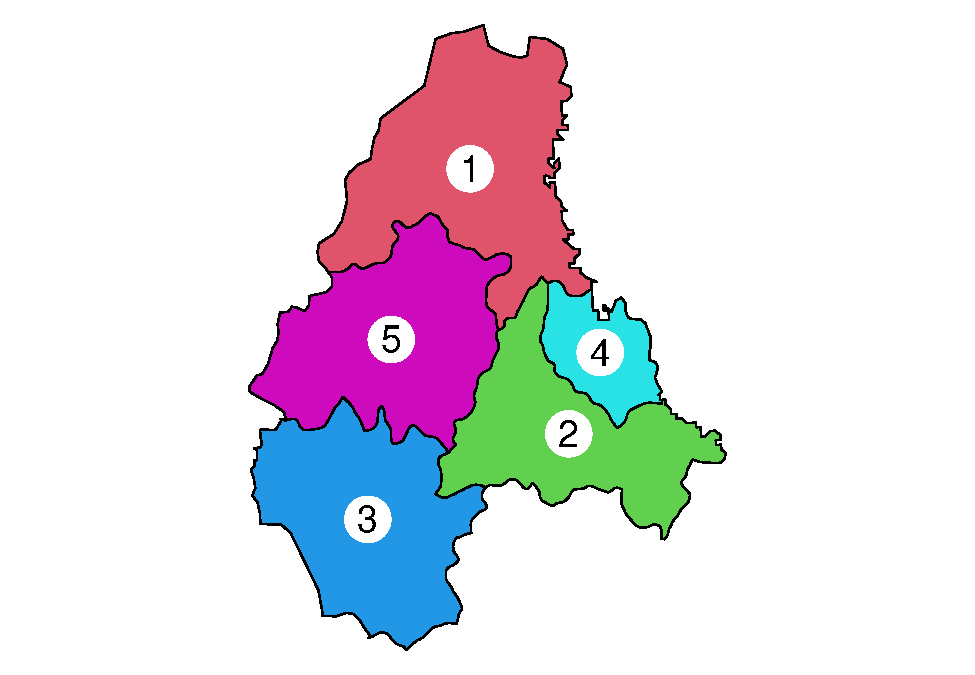
\includegraphics{modul_files/figure-latex/unnamed-chunk-31-1.pdf}

\begin{Shaded}
\begin{Highlighting}[]
\KeywordTok{moran.plot}\NormalTok{(petajawa}\OperatorTok{$}\NormalTok{Kemiskinan, wqueen, }\DataTypeTok{zero.policy=}\NormalTok{T, }\DataTypeTok{labels=}\NormalTok{petajawa}\OperatorTok{$}\NormalTok{KABKOT)}
\end{Highlighting}
\end{Shaded}

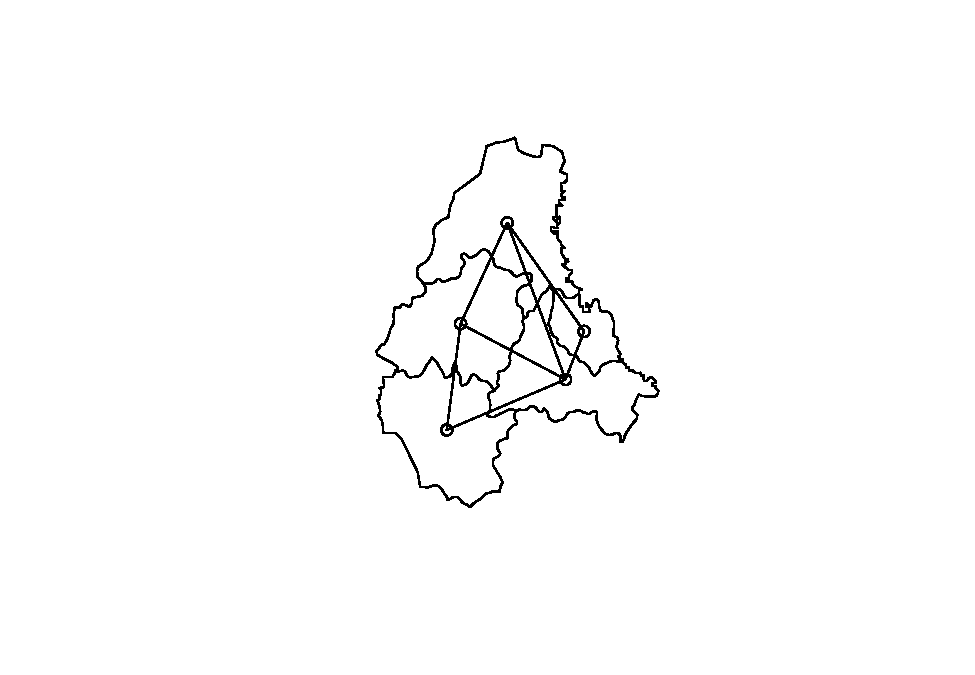
\includegraphics{modul_files/figure-latex/unnamed-chunk-32-1.pdf}

\hypertarget{sumber-pustaka}{%
\section{Sumber Pustaka}\label{sumber-pustaka}}

Agafonkin, V. (n.d.). Leaflet for R - Markers. rstudio.github.io. Retrieved from \url{https://rstudio.github.io/leaflet/markers.html}

Baumer, B.S., Kaplan, D.T., Horton, N.J. 2017. Modern Data Science with R. CRC Press.

UQ SLC Digital Team. (2020, April 16). Creating maps using R. Language Technology and Data Analysis Laboratory (LADAL). Retrieved from \url{https://slcladal.github.io/maps.html}

\hypertarget{pemodelan-dependensi-spasial}{%
\chapter{Pemodelan Dependensi Spasial}\label{pemodelan-dependensi-spasial}}

\hypertarget{model-spasial-global}{%
\section{Model Spasial Global}\label{model-spasial-global}}

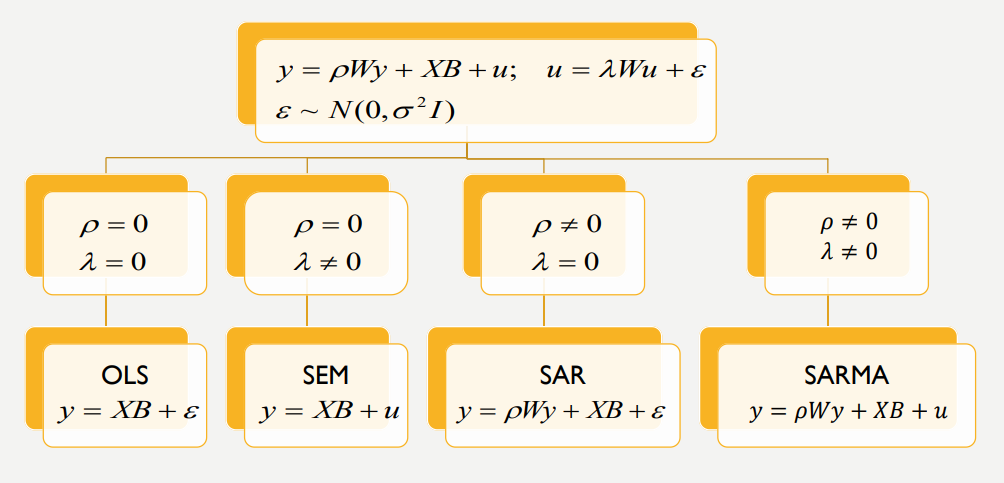
\includegraphics{D:/Research (eksternal dept)/pelatihan spasial (adj)/Modul Pelatihan Spasial/gambar 2.PNG}

Secara umum, tahapan pemodelan regresi spasial adalah sebagai berikut:

\begin{enumerate}
\def\labelenumi{(\arabic{enumi})}
\item
  Eksplorasi Data
\item
  Regresi Klasik \& Uji Asumsi
\item
  Matriks Pembobot Spasial
\item
  Uji Lagrange Multiplier
\item
  Regresi Spasial \& Uji Asumsi
\item
  Kebaikan Model
\end{enumerate}

Sebagai ilustrasi untuk menjelaskan tahapan tersebut, kita akan menggunakan data kemiskinan dan kependudukan di Pulau Jawa berikut ini:

\begin{enumerate}
\def\labelenumi{\arabic{enumi}.}
\item
  Data polygon (peta Pulau Jawa, dengan extension .shp)
\item
  Data frame (data persentase kemiskinan, PDRB, pendidikan Angka Melek Huruf, Pengeluaran perkapita, Ruta Penerima Raskin, Penduduk berusia 15-64, Harapan Lama Sekolah, dan Rata-Rata Lama Sekolah, diperoleh dari BPS)
\end{enumerate}

Seperti yang telah dijelaskan pada modul sebelumnya, impor data dapat dilakukan dengan program berikut ini.

\begin{Shaded}
\begin{Highlighting}[]
\NormalTok{datajawa =}\StringTok{ }\NormalTok{datajawa=}\KeywordTok{read.csv}\NormalTok{(}\StringTok{"Pulau Jawa.csv"}\NormalTok{, }\DataTypeTok{header=}\NormalTok{T, }\DataTypeTok{sep=}\StringTok{";"}\NormalTok{)}
\KeywordTok{head}\NormalTok{(datajawa)}
\end{Highlighting}
\end{Shaded}

\begin{verbatim}
##      Provinsi       Kabupaten.kota Longitude Latitude Kemiskinan   PDRB
## 1 DKI Jakarta     Kepulauan Seribu  106.5072  -5.7985      11.98 338.80
## 2             Kota Jakarta Selatan  106.8079  -6.2627       2.83 261.58
## 3               Kota Jakarta Timur  106.8995  -6.2249       3.14 155.53
## 4               Kota Jakarta Pusat  106.8279  -6.1801       3.59 692.24
## 5               Kota Jakarta Barat  106.7633  -6.1675       3.39 168.68
## 6               Kota Jakarta Utara  106.8926  -6.1555       5.35 271.85
##   Pendidikan    AMH Pengeluaran.Perkapita Ruta.Penerima.Raskin Penduduk.15.64
## 1       5.29 100.00                 68.80                55.34        86.2882
## 2       7.96 100.00                 46.63                 0.00        86.8031
## 3       2.91 100.00                 50.39                 0.00        86.9343
## 4       3.62 100.00                 50.87                 0.00        86.2032
## 5      25.02 100.00                 53.29                 0.00        87.4070
## 6      18.59  98.98                 51.12                 0.00        87.3943
##     HLS Rata.Rata.Lama.Sekolah
## 1 12.48                   8.46
## 2 13.31                  11.57
## 3 13.43                  11.64
## 4 13.23                  11.24
## 5 12.78                  10.38
## 6 12.61                  10.69
\end{verbatim}

Pada ilustrasi ini, pemodelan dilakukan untuk mengkaji peubah respon \textbf{persentase penduduk miskin tahun 2018 di pulau Jawa (\(Y\))} dengan menggunakan peubah \textbf{persentase Pendidikan yang ditamatkan di Bawah SD Tahun 2018(\(X\))}.

\begin{Shaded}
\begin{Highlighting}[]
\KeywordTok{library}\NormalTok{(spdep)}
\KeywordTok{library}\NormalTok{(rgdal)}
\KeywordTok{library}\NormalTok{(raster)}

\NormalTok{petajawa\textless{}{-}}\KeywordTok{readOGR}\NormalTok{(}\DataTypeTok{dsn=}\NormalTok{“directory tempat folder utk file .shp}\StringTok{", layer=“nama file shp"}\NormalTok{)}
\end{Highlighting}
\end{Shaded}

\hypertarget{eksplorasi-data}{%
\section{Eksplorasi Data}\label{eksplorasi-data}}

\begin{Shaded}
\begin{Highlighting}[]
\KeywordTok{plot}\NormalTok{(datajawa}\OperatorTok{$}\NormalTok{Pendidikan, datajawa}\OperatorTok{$}\NormalTok{Kemiskinan,}
  \DataTypeTok{xlab=}\StringTok{"Persentase Pendidikan yang ditamatkan di bawah SD Thn.2018"}\NormalTok{, }
  \DataTypeTok{ylab=}\StringTok{"Persentase Penduduk Miskin Thn.2018"}\NormalTok{,}
  \DataTypeTok{pch=}\DecValTok{20}\NormalTok{, }\DataTypeTok{col=}\StringTok{"orange"}\NormalTok{, }\DataTypeTok{cex=}\DecValTok{2}\NormalTok{)}
\end{Highlighting}
\end{Shaded}

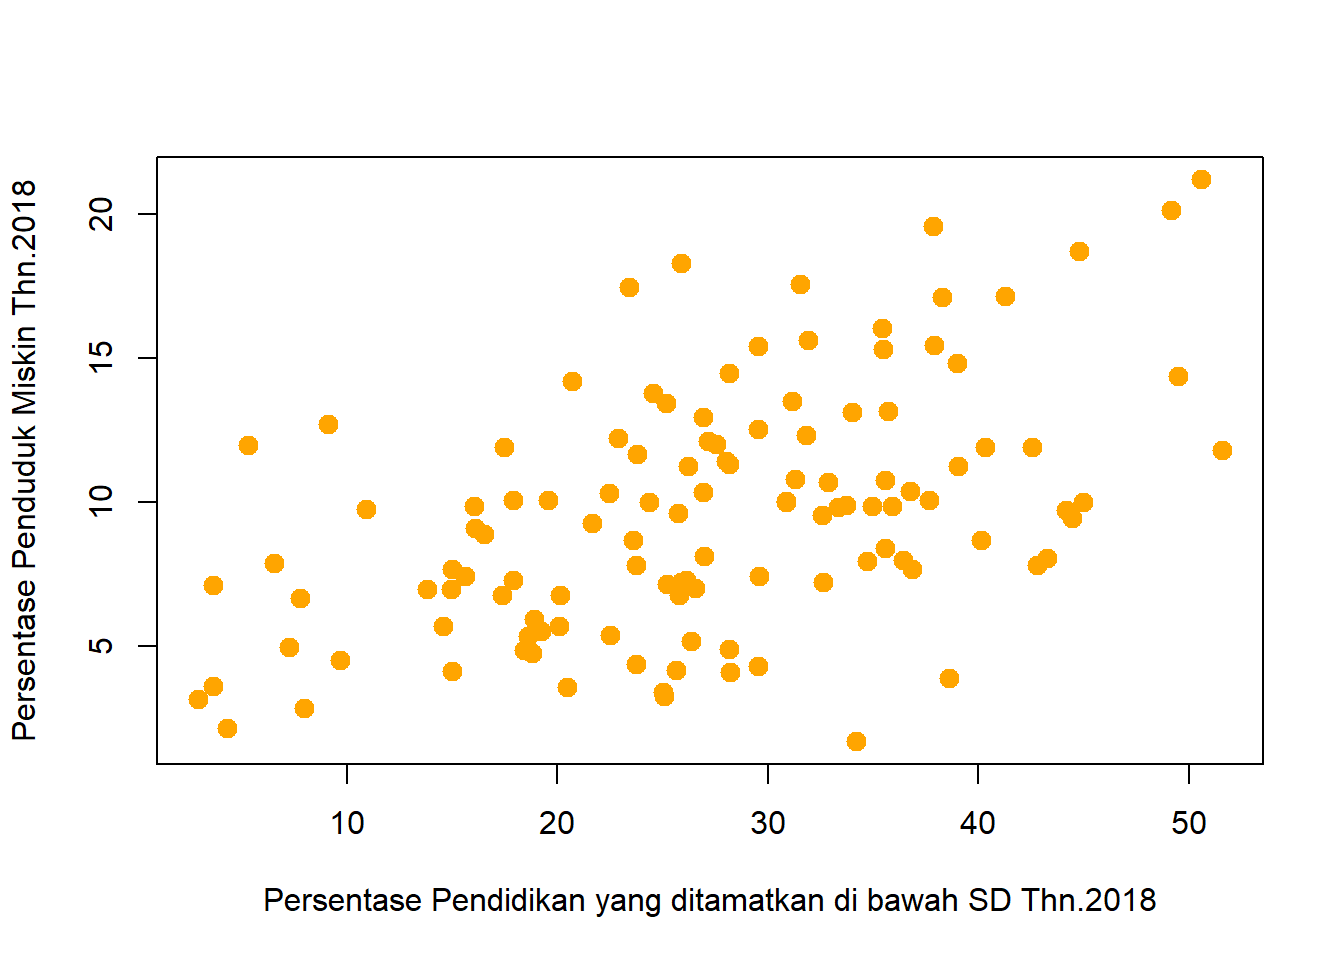
\includegraphics{modul_files/figure-latex/unnamed-chunk-36-1.pdf}

Plot tersebut memperlihatkan adanya pola hubungan linear positif antara persentase pendidikan yang ditamatkan di bawah SD terhadap persentase penduduk miskin di Pulau Jawa pada tahun 2018.

\begin{Shaded}
\begin{Highlighting}[]
\NormalTok{petajawa}\OperatorTok{$}\NormalTok{Kemiskinan\textless{}{-}}\StringTok{ }\NormalTok{datajawa}\OperatorTok{$}\NormalTok{Kemiskinan}
\NormalTok{k=}\DecValTok{16}
\NormalTok{colfunc \textless{}{-}}\StringTok{ }\KeywordTok{colorRampPalette}\NormalTok{(}\KeywordTok{c}\NormalTok{(}\StringTok{"green"}\NormalTok{, }\StringTok{"yellow"}\NormalTok{,}\StringTok{"red"}\NormalTok{))}
\NormalTok{color \textless{}{-}}\StringTok{ }\KeywordTok{colfunc}\NormalTok{(k)}
\KeywordTok{spplot}\NormalTok{(petajawa, }\StringTok{"Kemiskinan"}\NormalTok{, }\DataTypeTok{col.regions=}\NormalTok{color, }\DataTypeTok{main=}\StringTok{"Persentase Penduduk Miskin Tahun 2018"}\NormalTok{)}
\end{Highlighting}
\end{Shaded}

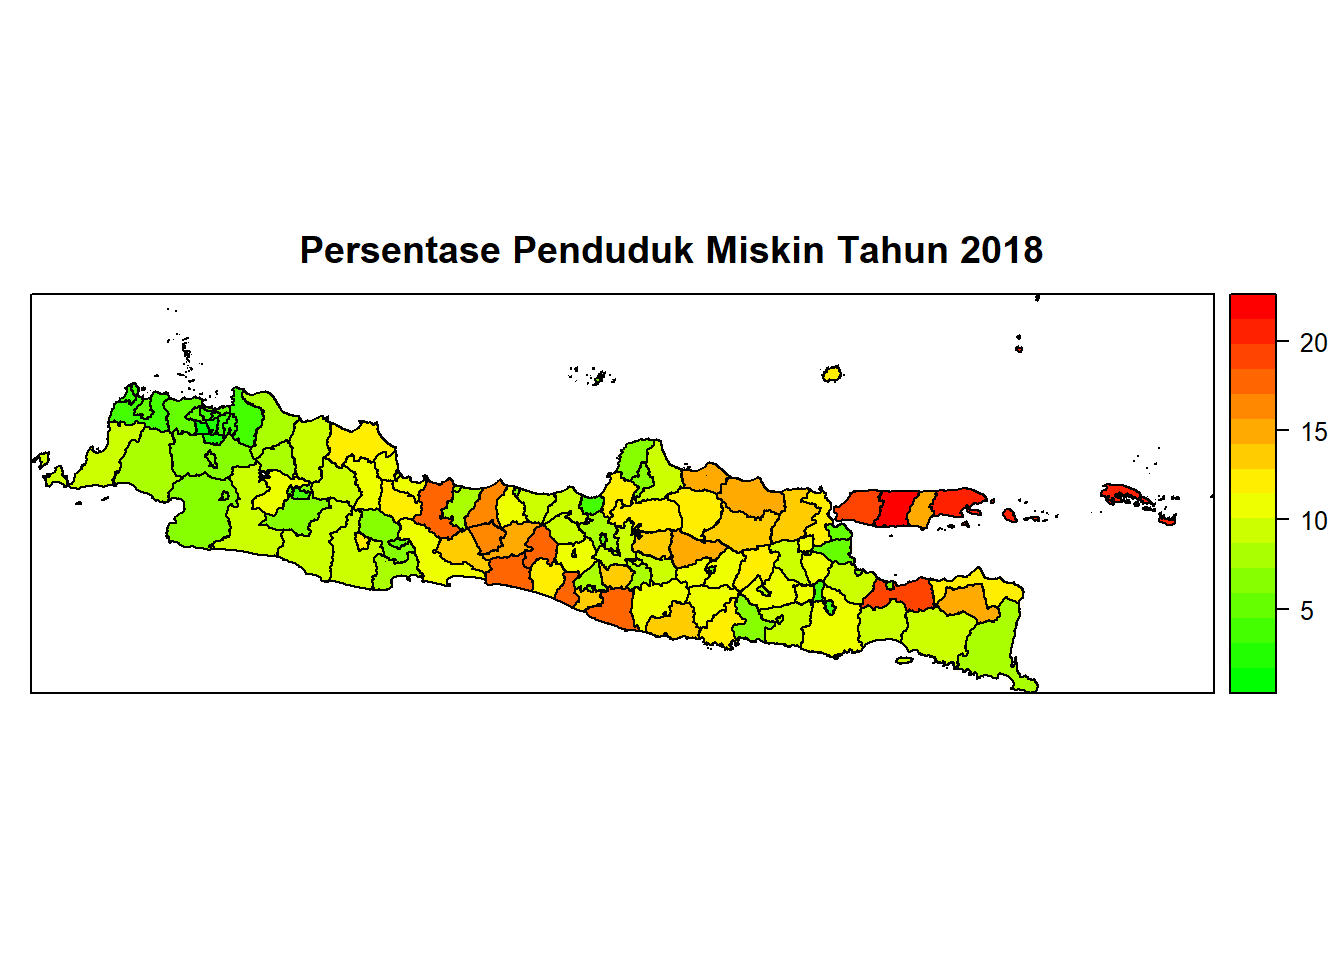
\includegraphics{modul_files/figure-latex/unnamed-chunk-37-1.pdf}

Berdasarkan plot di atas, dapat dilihat adanya kecenderungan pola bergerombol pada data persentase kemiskinan di kabupaten/kota di Pulau Jawa. Hal ini tampak dari gradasi warna yang cenderung mengumpul, seperti pada warna hijau, merah dan oranye.

\hypertarget{identifikasi-autokorelasi-pada-data}{%
\subsection{Identifikasi Autokorelasi pada Data}\label{identifikasi-autokorelasi-pada-data}}

\begin{Shaded}
\begin{Highlighting}[]
\NormalTok{w\textless{}{-}}\KeywordTok{poly2nb}\NormalTok{(petajawa)}
\NormalTok{ww\textless{}{-}}\KeywordTok{nb2listw}\NormalTok{(w, }\DataTypeTok{zero.policy=}\NormalTok{T)}
\KeywordTok{moran}\NormalTok{(datajawa}\OperatorTok{$}\NormalTok{Kemiskinan, ww, }\DataTypeTok{n=}\KeywordTok{length}\NormalTok{(ww}\OperatorTok{$}\NormalTok{neighbours), }
      \DataTypeTok{S0=}\KeywordTok{Szero}\NormalTok{(ww), }\DataTypeTok{zero.policy=}\NormalTok{T)}
\end{Highlighting}
\end{Shaded}

\begin{verbatim}
## $I
## [1] 0.5214426
## 
## $K
## [1] 2.853193
\end{verbatim}

\begin{Shaded}
\begin{Highlighting}[]
\KeywordTok{moran.test}\NormalTok{(datajawa}\OperatorTok{$}\NormalTok{Kemiskinan, ww,}\DataTypeTok{randomisation=}\NormalTok{T, }
           \DataTypeTok{alternative=}\StringTok{"greater"}\NormalTok{, }\DataTypeTok{zero.policy=}\NormalTok{T)}
\end{Highlighting}
\end{Shaded}

\begin{verbatim}
## 
##  Moran I test under randomisation
## 
## data:  datajawa$Kemiskinan  
## weights: ww  n reduced by no-neighbour observations
##   
## 
## Moran I statistic standard deviate = 7.7638, p-value = 4.12e-15
## alternative hypothesis: greater
## sample estimates:
## Moran I statistic       Expectation          Variance 
##       0.517060772      -0.008547009       0.004583226
\end{verbatim}

\begin{Shaded}
\begin{Highlighting}[]
\KeywordTok{moran.plot}\NormalTok{(datajawa}\OperatorTok{$}\NormalTok{Kemiskinan, ww, }\DataTypeTok{labels=}\NormalTok{petajawa}\OperatorTok{$}\NormalTok{KABKOT, }\DataTypeTok{zero.policy=}\NormalTok{T)}
\end{Highlighting}
\end{Shaded}

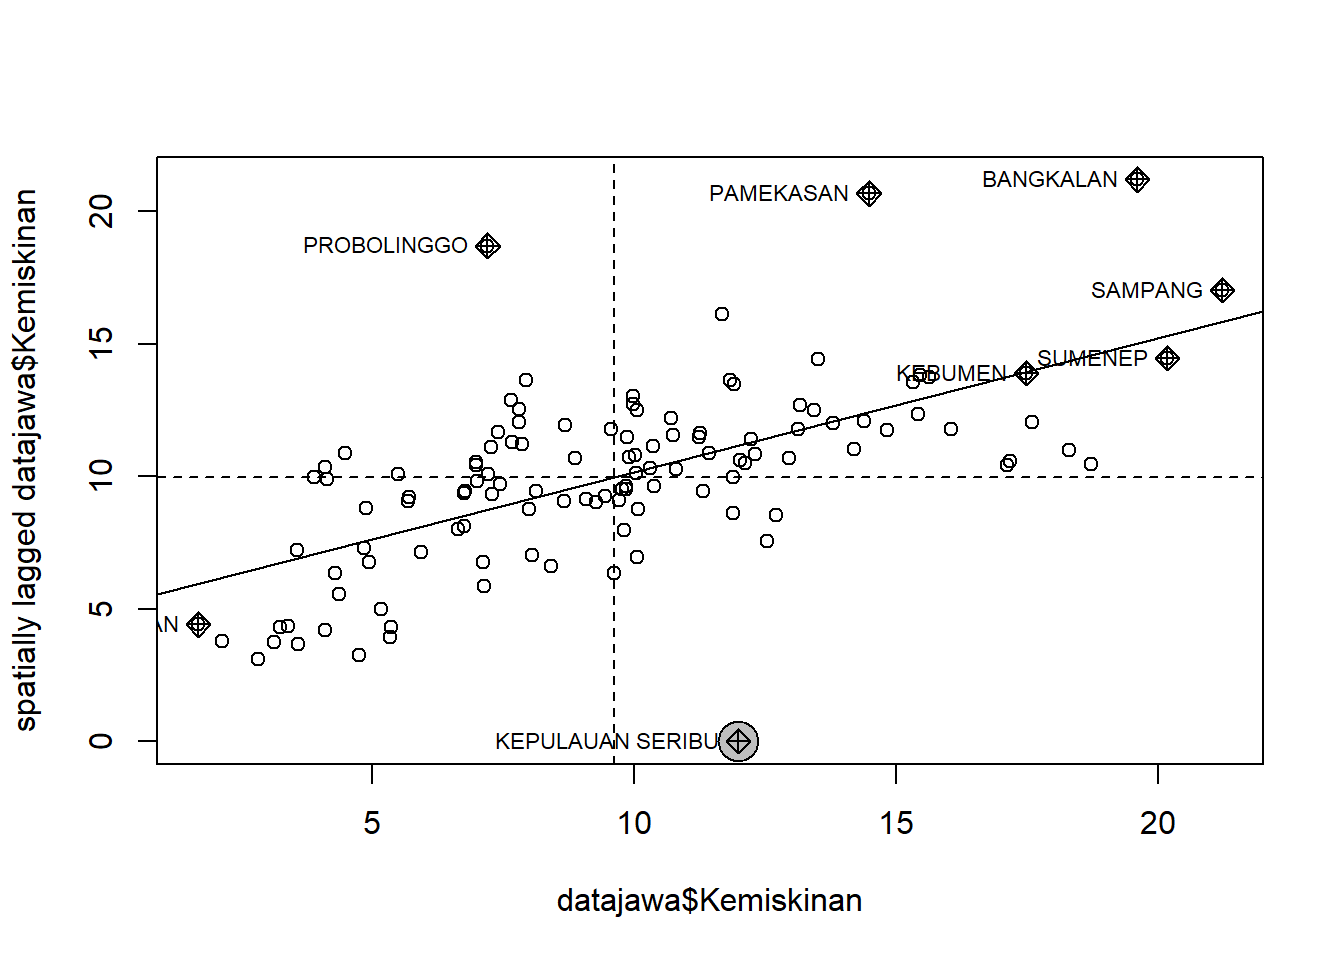
\includegraphics{modul_files/figure-latex/unnamed-chunk-39-1.pdf}

\hypertarget{pemodelan-regresi-klasik}{%
\section{Pemodelan Regresi Klasik}\label{pemodelan-regresi-klasik}}

Pemodelan regresi dapat dilakukan menggunakan fungsi \texttt{lm} berikut.

\begin{Shaded}
\begin{Highlighting}[]
\NormalTok{reg.klasik =}\StringTok{ }\KeywordTok{lm}\NormalTok{(Kemiskinan}\OperatorTok{\textasciitilde{}}\NormalTok{Pendidikan, }\DataTypeTok{data =}\NormalTok{ datajawa)}
\NormalTok{err.regklasik\textless{}{-}}\KeywordTok{residuals}\NormalTok{(reg.klasik)}
\KeywordTok{summary}\NormalTok{(reg.klasik)}
\end{Highlighting}
\end{Shaded}

\begin{verbatim}
## 
## Call:
## lm(formula = Kemiskinan ~ Pendidikan, data = datajawa)
## 
## Residuals:
##     Min      1Q  Median      3Q     Max 
## -9.3117 -2.6659 -0.3763  2.2998  8.8844 
## 
## Coefficients:
##             Estimate Std. Error t value Pr(>|t|)    
## (Intercept)  4.50549    0.89314   5.045 1.68e-06 ***
## Pendidikan   0.18965    0.03066   6.186 9.37e-09 ***
## ---
## Signif. codes:  0 '***' 0.001 '**' 0.01 '*' 0.05 '.' 0.1 ' ' 1
## 
## Residual standard error: 3.671 on 117 degrees of freedom
## Multiple R-squared:  0.2464, Adjusted R-squared:   0.24 
## F-statistic: 38.26 on 1 and 117 DF,  p-value: 9.373e-09
\end{verbatim}

\begin{Shaded}
\begin{Highlighting}[]
\KeywordTok{cor}\NormalTok{(datajawa}\OperatorTok{$}\NormalTok{Kemiskinan, }\KeywordTok{fitted}\NormalTok{(reg.klasik))}\OperatorTok{\^{}}\DecValTok{2}
\end{Highlighting}
\end{Shaded}

\begin{verbatim}
## [1] 0.2464408
\end{verbatim}

\hypertarget{diagnostik-model}{%
\section{Diagnostik Model}\label{diagnostik-model}}

\hypertarget{kenormalan-sisaan}{%
\subsection{Kenormalan Sisaan}\label{kenormalan-sisaan}}

\begin{Shaded}
\begin{Highlighting}[]
\KeywordTok{library}\NormalTok{(nortest)}
\KeywordTok{library}\NormalTok{(car)}
\KeywordTok{library}\NormalTok{(DescTools)}
\KeywordTok{library}\NormalTok{(lmtest)}
\KeywordTok{shapiro.test}\NormalTok{(err.regklasik)}
\end{Highlighting}
\end{Shaded}

\begin{verbatim}
## 
##  Shapiro-Wilk normality test
## 
## data:  err.regklasik
## W = 0.98607, p-value = 0.2608
\end{verbatim}

\begin{Shaded}
\begin{Highlighting}[]
\KeywordTok{par}\NormalTok{(}\DataTypeTok{mfrow=}\KeywordTok{c}\NormalTok{(}\DecValTok{1}\NormalTok{,}\DecValTok{2}\NormalTok{))}
\KeywordTok{hist}\NormalTok{(err.regklasik)}
\NormalTok{car}\OperatorTok{::}\KeywordTok{qqPlot}\NormalTok{(}\KeywordTok{residuals}\NormalTok{(reg.klasik))}
\end{Highlighting}
\end{Shaded}

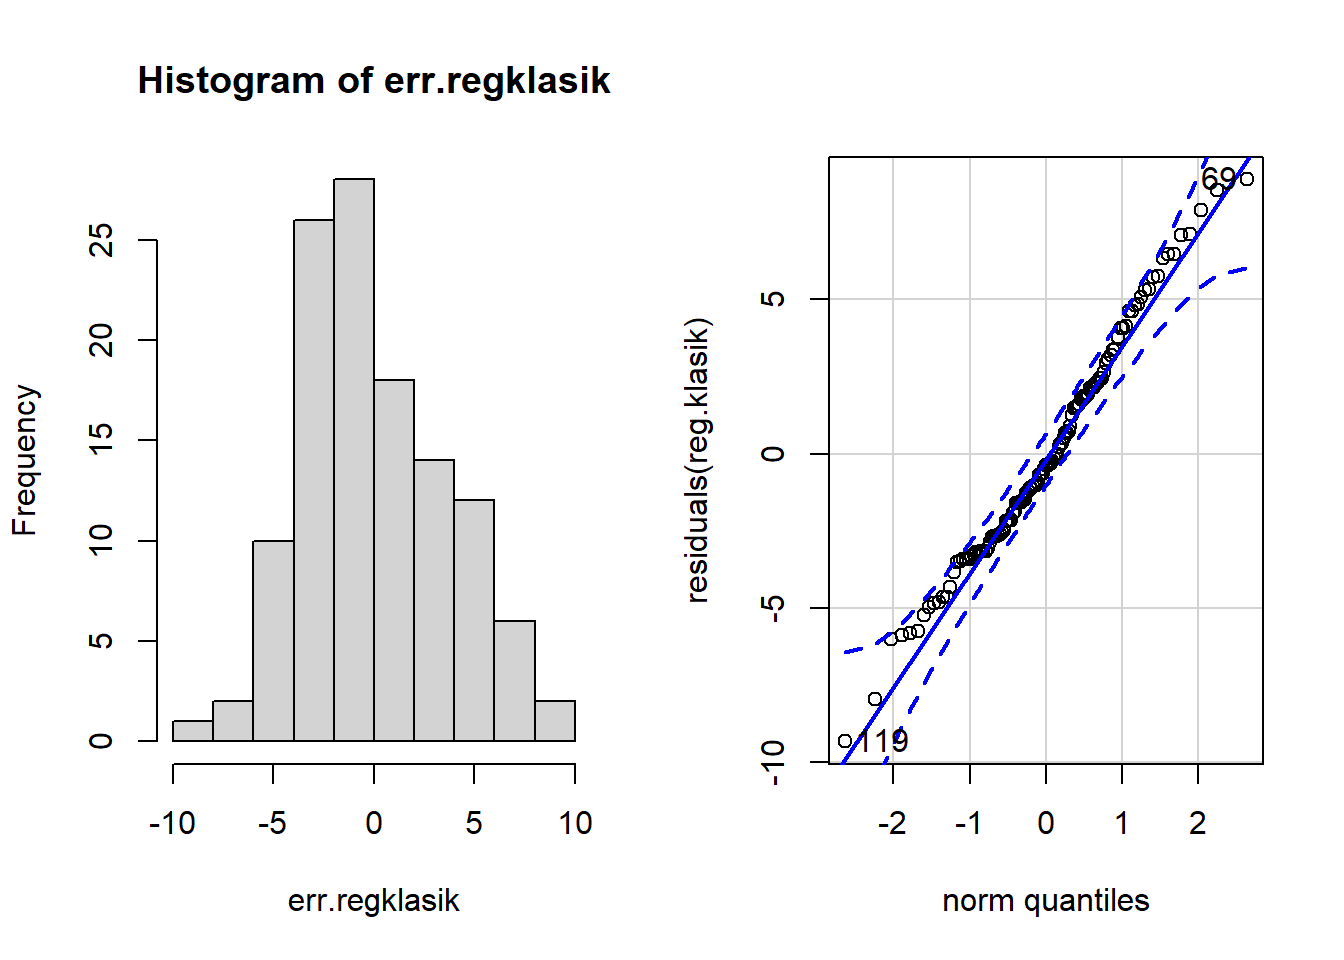
\includegraphics{modul_files/figure-latex/unnamed-chunk-41-1.pdf}

\begin{verbatim}
## [1] 119  69
\end{verbatim}

\begin{quote}
H0: galat model menyebar normal
\end{quote}

\begin{quote}
H1: galat model tidak menyebar normal
\end{quote}

\hypertarget{kehomogenan-ragam-sisaan}{%
\subsection{Kehomogenan Ragam Sisaan}\label{kehomogenan-ragam-sisaan}}

\begin{Shaded}
\begin{Highlighting}[]
\KeywordTok{plot}\NormalTok{(}\KeywordTok{fitted}\NormalTok{(reg.klasik), }\KeywordTok{residuals}\NormalTok{(reg.klasik))}
\end{Highlighting}
\end{Shaded}

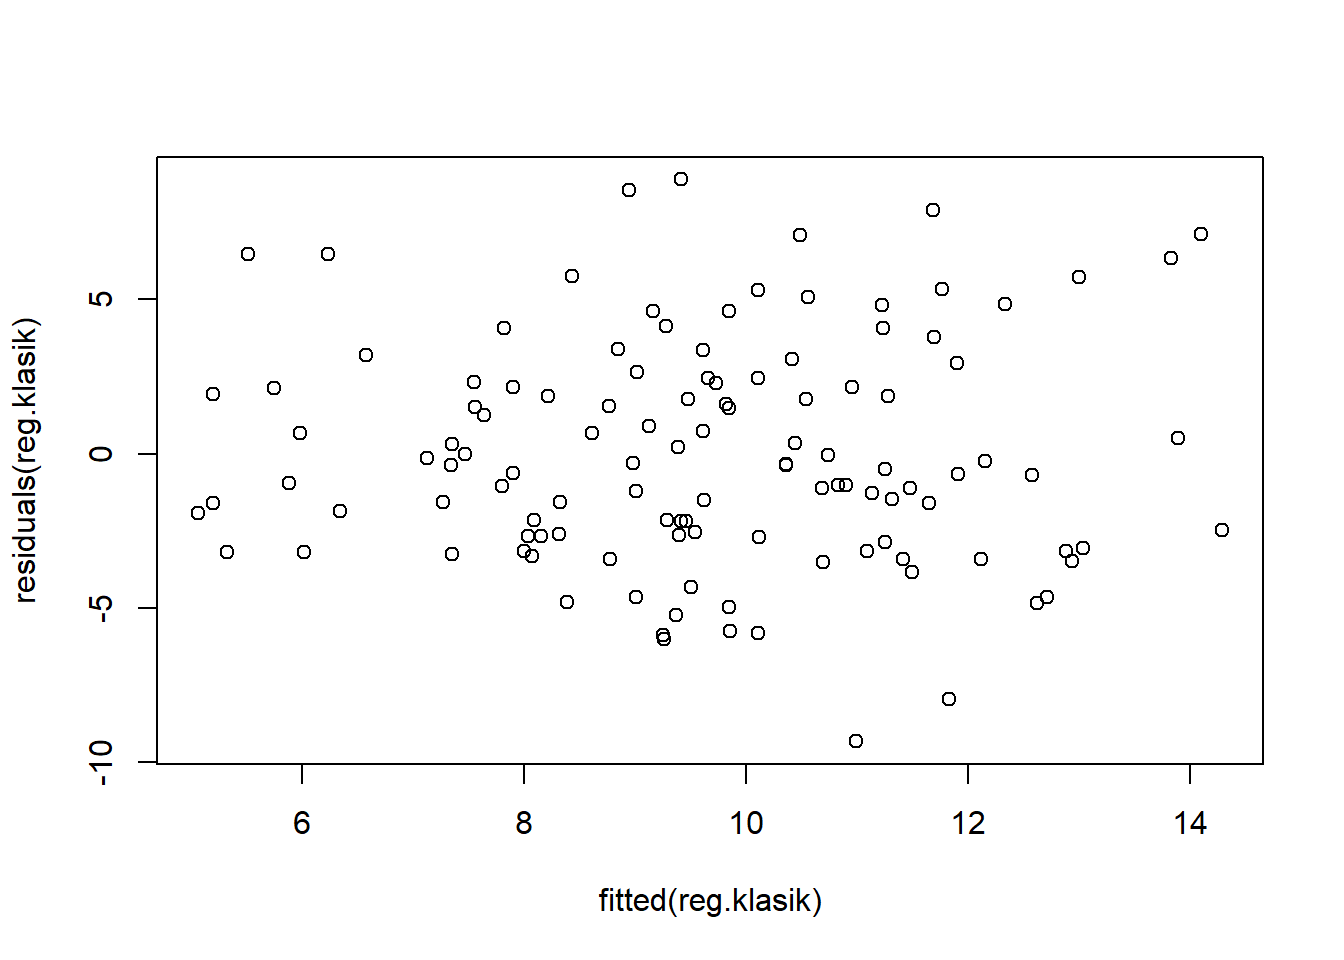
\includegraphics{modul_files/figure-latex/unnamed-chunk-42-1.pdf}

\begin{Shaded}
\begin{Highlighting}[]
\KeywordTok{bptest}\NormalTok{(reg.klasik)}
\end{Highlighting}
\end{Shaded}

\begin{verbatim}
## 
##  studentized Breusch-Pagan test
## 
## data:  reg.klasik
## BP = 3.979, df = 1, p-value = 0.04607
\end{verbatim}

\begin{quote}
H0: ragam galat homogen
\end{quote}

\begin{quote}
H1: ragam galat tidak homogen
\end{quote}

\hypertarget{kebebasan-sisaan}{%
\subsection{Kebebasan Sisaan}\label{kebebasan-sisaan}}

Uji kebebasan sisaan pada data spasial dapat dilakukan dengan uji moran menggunakan fungsi berikut.

\begin{Shaded}
\begin{Highlighting}[]
\NormalTok{w\textless{}{-}}\KeywordTok{poly2nb}\NormalTok{(petajawa)}
\NormalTok{ww\textless{}{-}}\KeywordTok{nb2listw}\NormalTok{(w, }\DataTypeTok{zero.policy =}\NormalTok{T)}
\KeywordTok{lm.morantest}\NormalTok{(reg.klasik, ww, }\DataTypeTok{alternative=}\StringTok{"two.sided"}\NormalTok{, }\DataTypeTok{zero.policy =}\NormalTok{ T)}
\end{Highlighting}
\end{Shaded}

\begin{verbatim}
## 
##  Global Moran I for regression residuals
## 
## data:  
## model: lm(formula = Kemiskinan ~ Pendidikan, data = datajawa)
## weights: ww
## 
## Moran I statistic standard deviate = 5.3932, p-value = 6.922e-08
## alternative hypothesis: two.sided
## sample estimates:
## Observed Moran I      Expectation         Variance 
##      0.351747300     -0.011502703      0.004536512
\end{verbatim}

Selain menggunakan fungsi \texttt{lm.morantest}, uji moran dapat dilakukan menggunakan fungsi \texttt{moran.test} seperti yang dibahas pada modul pertemuan sebelumnya. Perbedaannya adalah pada fungsi pertama, input yang digunakan adalah objek \texttt{lm}, sedangkan pada fungsi kedua, yang digunakan sebagai input adalah data sisaan model.

\begin{Shaded}
\begin{Highlighting}[]
\KeywordTok{moran.test}\NormalTok{(err.regklasik, ww,}\DataTypeTok{randomisation=}\NormalTok{F, }\DataTypeTok{alternative=}\StringTok{"two.sided"}\NormalTok{, }\DataTypeTok{zero.policy=}\NormalTok{T)}
\end{Highlighting}
\end{Shaded}

\begin{verbatim}
## 
##  Moran I test under normality
## 
## data:  err.regklasik  
## weights: ww  n reduced by no-neighbour observations
##   
## 
## Moran I statistic standard deviate = 5.3242, p-value = 1.014e-07
## alternative hypothesis: two.sided
## sample estimates:
## Moran I statistic       Expectation          Variance 
##       0.351747300      -0.008547009       0.004579345
\end{verbatim}

Terlihat pada output bahwa hasil kedua tes menunjukkan kesimpulan yang sama, yaitu tolak H0 yang menyatakan bahwa tidak terdapat autokorelasi pada sisaan model regresi klasik pada taraf nyata 5\%. Oleh karenanya, untuk mencari model yang lebih baik, kita dapat melakukan uji LM (lagrange multiplier) untuk mengidentifikasi model dependensi spasial yang dapat digunakan pada kasus ini.

\hypertarget{uji-lagrange-multiplier}{%
\section{Uji Lagrange Multiplier}\label{uji-lagrange-multiplier}}

\begin{Shaded}
\begin{Highlighting}[]
\NormalTok{LM\textless{}{-}}\KeywordTok{lm.LMtests}\NormalTok{(reg.klasik, }\KeywordTok{nb2listw}\NormalTok{(w, }\DataTypeTok{style=}\StringTok{"W"}\NormalTok{, }\DataTypeTok{zero.policy=}\NormalTok{T),}
               \DataTypeTok{test=}\KeywordTok{c}\NormalTok{(}\StringTok{"LMerr"}\NormalTok{, }\StringTok{"LMlag"}\NormalTok{,}\StringTok{"RLMerr"}\NormalTok{,}\StringTok{"RLMlag"}\NormalTok{,}\StringTok{"SARMA"}\NormalTok{), }\DataTypeTok{zero.policy=}\NormalTok{T)}
\KeywordTok{summary}\NormalTok{(LM)}
\end{Highlighting}
\end{Shaded}

\begin{verbatim}
##  Lagrange multiplier diagnostics for spatial dependence
## data:  
## model: lm(formula = Kemiskinan ~ Pendidikan, data = datajawa)
## weights: nb2listw(w, style = "W", zero.policy = T)
##  
##        statistic parameter   p.value    
## LMerr    26.4886         1 2.651e-07 ***
## LMlag    27.2100         1 1.825e-07 ***
## RLMerr    1.4217         1    0.2331    
## RLMlag    2.1431         1    0.1432    
## SARMA    28.6317         2 6.063e-07 ***
## ---
## Signif. codes:  0 '***' 0.001 '**' 0.01 '*' 0.05 '.' 0.1 ' ' 1
\end{verbatim}

Output memperlihatkan bahwa hasil uji model SEM dan SAR sama-sama signifikan pada taraf 5\%. Selanjutnya, hasil uji robust keduanya ternyata sama-sama tidak signifikan. Berdasarkan skema tersebut, kita dapat mencoba kandidat model SARMA atau GSM. Namun demikian, ada pula pendapat yang menyarankan agar kita mengambil kandidat model dengan p-value terkecil, pada kasus ini p-value terkecil juga terdapat pada model SARMA atau GSM.

Mohon diingat bahwa pada ilustrasi yang kita lakukan saat ini, kita hanya menggunakan satu peubah bebas sehingga kita tidak perlu mengkhawatirkan masalah multikolinieritas. Pada saat Anda memiliki lebih dari satu peubah bebas, pastikan Anda juga memperhatikan multikolinieritas pada model. Pemeriksaan dapat dilakukan dengan fungsi \texttt{vif()} pada package \texttt{car}.

\hypertarget{pemodelan-regresi-spasial}{%
\section{Pemodelan Regresi Spasial}\label{pemodelan-regresi-spasial}}

Pada modul ini, untuk kepentingan pembelajaran, kita akan mencoba ketiga model, SEM, SAR, dan SARMA, meskipun pada prakteknya, Anda hanya perlu memodelkan yang menurut Anda terbaik saja.

\begin{Shaded}
\begin{Highlighting}[]
\NormalTok{w\textless{}{-}}\KeywordTok{poly2nb}\NormalTok{(petajawa)}
\NormalTok{ww\textless{}{-}}\KeywordTok{nb2listw}\NormalTok{(w, }\DataTypeTok{zero.policy=}\NormalTok{T)}
\end{Highlighting}
\end{Shaded}

\hypertarget{model-sem}{%
\subsection{Model SEM}\label{model-sem}}

\begin{Shaded}
\begin{Highlighting}[]
\KeywordTok{library}\NormalTok{(spatialreg)}

\NormalTok{sem\textless{}{-}}\KeywordTok{errorsarlm}\NormalTok{(Kemiskinan}\OperatorTok{\textasciitilde{}}\NormalTok{Pendidikan,}\DataTypeTok{data=}\NormalTok{datajawa,ww, }\DataTypeTok{zero.policy=}\NormalTok{T)}
\KeywordTok{summary}\NormalTok{(sem)}
\end{Highlighting}
\end{Shaded}

\begin{verbatim}
## 
## Call:errorsarlm(formula = Kemiskinan ~ Pendidikan, data = datajawa, 
##     listw = ww, zero.policy = T)
## 
## Residuals:
##      Min       1Q   Median       3Q      Max 
## -7.04950 -1.86484 -0.43797  1.87675  8.14992 
## 
## Type: error 
## Regions with no neighbours included:
##  0 
## Coefficients: (asymptotic standard errors) 
##             Estimate Std. Error z value  Pr(>|z|)
## (Intercept) 6.359121   0.958495  6.6345 3.256e-11
## Pendidikan  0.114932   0.029332  3.9183 8.918e-05
## 
## Lambda: 0.57487, LR test value: 29.606, p-value: 5.2937e-08
## Asymptotic standard error: 0.083992
##     z-value: 6.8443, p-value: 7.6856e-12
## Wald statistic: 46.844, p-value: 7.6857e-12
## 
## Log likelihood: -307.7876 for error model
## ML residual variance (sigma squared): 9.4425, (sigma: 3.0729)
## Number of observations: 119 
## Number of parameters estimated: 4 
## AIC: 623.58, (AIC for lm: 651.18)
\end{verbatim}

\begin{Shaded}
\begin{Highlighting}[]
\NormalTok{pseudoR2.sem\textless{}{-}}\KeywordTok{cor}\NormalTok{(datajawa}\OperatorTok{$}\NormalTok{Kemiskinan, }\KeywordTok{fitted}\NormalTok{(sem))}\OperatorTok{\^{}}\DecValTok{2}
\NormalTok{pseudoR2.sem}
\end{Highlighting}
\end{Shaded}

\begin{verbatim}
## [1] 0.4786585
\end{verbatim}

Output di atas menunjukkan bahwa koefisien Lambda signifikan pada taraf nyata 5\% ( p-value = 5.2937e-08 ). AIC model SEM adalah sebesar 623.58, dengan pseudo-\(R^2=0.4787\) Selanjutnya kita akan coba memeriksa sisaan model SEM ini.

\begin{Shaded}
\begin{Highlighting}[]
\KeywordTok{library}\NormalTok{(nortest)}
\NormalTok{err.sem\textless{}{-}}\KeywordTok{residuals}\NormalTok{(sem)}
\KeywordTok{shapiro.test}\NormalTok{(err.sem)}
\end{Highlighting}
\end{Shaded}

\begin{verbatim}
## 
##  Shapiro-Wilk normality test
## 
## data:  err.sem
## W = 0.98234, p-value = 0.1208
\end{verbatim}

\begin{Shaded}
\begin{Highlighting}[]
\KeywordTok{bptest.sarlm}\NormalTok{(sem)}
\end{Highlighting}
\end{Shaded}

\begin{verbatim}
## 
##  studentized Breusch-Pagan test
## 
## data:  
## BP = 4.1883, df = 1, p-value = 0.0407
\end{verbatim}

\begin{Shaded}
\begin{Highlighting}[]
\KeywordTok{moran.test}\NormalTok{(err.sem, ww, }\DataTypeTok{alternative=}\StringTok{"two.sided"}\NormalTok{, }\DataTypeTok{zero.policy=}\NormalTok{T)}
\end{Highlighting}
\end{Shaded}

\begin{verbatim}
## 
##  Moran I test under randomisation
## 
## data:  err.sem  
## weights: ww  n reduced by no-neighbour observations
##   
## 
## Moran I statistic standard deviate = -0.53535, p-value = 0.5924
## alternative hypothesis: two.sided
## sample estimates:
## Moran I statistic       Expectation          Variance 
##      -0.044773446      -0.008547009       0.004579087
\end{verbatim}

Terlihat pada output di atas bahwa sisaan memenuhi asumsi kenormalan dan asumsi kebebasan.

\hypertarget{model-sar}{%
\subsection{Model SAR}\label{model-sar}}

\begin{Shaded}
\begin{Highlighting}[]
\NormalTok{sar\textless{}{-}}\KeywordTok{lagsarlm}\NormalTok{(Kemiskinan}\OperatorTok{\textasciitilde{}}\NormalTok{Pendidikan,}\DataTypeTok{data=}\NormalTok{datajawa,ww, }\DataTypeTok{zero.policy=}\NormalTok{T)}
\KeywordTok{summary}\NormalTok{(sar)}
\end{Highlighting}
\end{Shaded}

\begin{verbatim}
## 
## Call:lagsarlm(formula = Kemiskinan ~ Pendidikan, data = datajawa, 
##     listw = ww, zero.policy = T)
## 
## Residuals:
##      Min       1Q   Median       3Q      Max 
## -7.17361 -1.97250 -0.56646  1.82449  9.57815 
## 
## Type: lag 
## Regions with no neighbours included:
##  0 
## Coefficients: (asymptotic standard errors) 
##             Estimate Std. Error z value  Pr(>|z|)
## (Intercept) 1.779095   0.992235  1.7930   0.07297
## Pendidikan  0.117724   0.027717  4.2473 2.164e-05
## 
## Rho: 0.46783, LR test value: 25.624, p-value: 4.1491e-07
## Asymptotic standard error: 0.087013
##     z-value: 5.3766, p-value: 7.5901e-08
## Wald statistic: 28.908, p-value: 7.5901e-08
## 
## Log likelihood: -309.7788 for lag model
## ML residual variance (sigma squared): 10.098, (sigma: 3.1777)
## Number of observations: 119 
## Number of parameters estimated: 4 
## AIC: 627.56, (AIC for lm: 651.18)
## LM test for residual autocorrelation
## test value: 0.014268, p-value: 0.90492
\end{verbatim}

\begin{Shaded}
\begin{Highlighting}[]
\NormalTok{pseudoR2.sar\textless{}{-}}\KeywordTok{cor}\NormalTok{(datajawa}\OperatorTok{$}\NormalTok{Kemiskinan, }\KeywordTok{fitted}\NormalTok{(sar))}\OperatorTok{\^{}}\DecValTok{2}
\NormalTok{pseudoR2.sar}
\end{Highlighting}
\end{Shaded}

\begin{verbatim}
## [1] 0.4292466
\end{verbatim}

Output di atas memperlihatkan bahwa koefisien Rho pada model SAR signifikan, dengan nilai AIC sebesar 627.56 dengan pseudo-\(R^2=0.4292\) . Selain itu, terlihat pula hasil uji autokorelasi pada sisaan model memperlihatkan nilai p-value sebesar 0.90492, artinya tidak terdapat autokorelasi pada sisaan.

\begin{Shaded}
\begin{Highlighting}[]
\NormalTok{err.sar\textless{}{-}}\KeywordTok{residuals}\NormalTok{(sar)}
\KeywordTok{shapiro.test}\NormalTok{(err.sar)}
\end{Highlighting}
\end{Shaded}

\begin{verbatim}
## 
##  Shapiro-Wilk normality test
## 
## data:  err.sar
## W = 0.98005, p-value = 0.07421
\end{verbatim}

\begin{Shaded}
\begin{Highlighting}[]
\KeywordTok{bptest.sarlm}\NormalTok{(sar)}
\end{Highlighting}
\end{Shaded}

\begin{verbatim}
## 
##  studentized Breusch-Pagan test
## 
## data:  
## BP = 1.6725, df = 1, p-value = 0.1959
\end{verbatim}

\begin{Shaded}
\begin{Highlighting}[]
\KeywordTok{moran.test}\NormalTok{(err.sar, ww, }\DataTypeTok{alternative=}\StringTok{"two.sided"}\NormalTok{, }\DataTypeTok{zero.policy=}\NormalTok{T)}
\end{Highlighting}
\end{Shaded}

\begin{verbatim}
## 
##  Moran I test under randomisation
## 
## data:  err.sar  
## weights: ww  n reduced by no-neighbour observations
##   
## 
## Moran I statistic standard deviate = 0.18303, p-value = 0.8548
## alternative hypothesis: two.sided
## sample estimates:
## Moran I statistic       Expectation          Variance 
##       0.003823646      -0.008547009       0.004567919
\end{verbatim}

Berdasarkan output di atas, pada taraf 5\% dapat disimpulkan bahwa sisaan model memenuhi asumsi kenormalan, kehomogenan ragam, dan kebebasan.

\hypertarget{model-gsmsarma}{%
\subsection{Model GSM/SARMA}\label{model-gsmsarma}}

\begin{Shaded}
\begin{Highlighting}[]
\NormalTok{gsm\textless{}{-}}\KeywordTok{sacsarlm}\NormalTok{(Kemiskinan}\OperatorTok{\textasciitilde{}}\NormalTok{Pendidikan,}\DataTypeTok{data=}\NormalTok{datajawa,ww, }\DataTypeTok{zero.policy=}\NormalTok{T)}
\KeywordTok{summary}\NormalTok{(gsm)}
\end{Highlighting}
\end{Shaded}

\begin{verbatim}
## 
## Call:sacsarlm(formula = Kemiskinan ~ Pendidikan, data = datajawa, 
##     listw = ww, zero.policy = T)
## 
## Residuals:
##      Min       1Q   Median       3Q      Max 
## -6.20932 -1.69855 -0.38001  1.70634  7.26252 
## 
## Type: sac 
## Coefficients: (asymptotic standard errors) 
##              Estimate Std. Error z value Pr(>|z|)
## (Intercept) 10.338070   1.750226  5.9067 3.49e-09
## Pendidikan   0.099813   0.027137  3.6781 0.000235
## 
## Rho: -0.43058
## Asymptotic standard error: 0.14723
##     z-value: -2.9246, p-value: 0.0034494
## Lambda: 0.79882
## Asymptotic standard error: 0.069513
##     z-value: 11.492, p-value: < 2.22e-16
## 
## LR test value: 34.317, p-value: 3.5325e-08
## 
## Log likelihood: -305.432 for sac model
## ML residual variance (sigma squared): 7.7401, (sigma: 2.7821)
## Number of observations: 119 
## Number of parameters estimated: 5 
## AIC: 620.86, (AIC for lm: 651.18)
\end{verbatim}

\begin{Shaded}
\begin{Highlighting}[]
\NormalTok{pseudoR2.gsm\textless{}{-}}\KeywordTok{cor}\NormalTok{(datajawa}\OperatorTok{$}\NormalTok{Kemiskinan, }\KeywordTok{fitted}\NormalTok{(gsm))}\OperatorTok{\^{}}\DecValTok{2}
\NormalTok{pseudoR2.gsm}
\end{Highlighting}
\end{Shaded}

\begin{verbatim}
## [1] 0.5933811
\end{verbatim}

Output di atas memperlihatkan bahwa kedua koefisien dependensi spasial, Rho dan Lambda signifikan. AIC model SARMA adalah sebesar 620.86 dengan pseudo-\(R^2=0.5934\)

\begin{Shaded}
\begin{Highlighting}[]
\NormalTok{err.gsm\textless{}{-}}\KeywordTok{residuals}\NormalTok{(gsm)}
\KeywordTok{shapiro.test}\NormalTok{(err.gsm)}
\end{Highlighting}
\end{Shaded}

\begin{verbatim}
## 
##  Shapiro-Wilk normality test
## 
## data:  err.gsm
## W = 0.98527, p-value = 0.2219
\end{verbatim}

\begin{Shaded}
\begin{Highlighting}[]
\KeywordTok{bptest.sarlm}\NormalTok{(gsm)}
\end{Highlighting}
\end{Shaded}

\begin{verbatim}
## 
##  studentized Breusch-Pagan test
## 
## data:  
## BP = 2.3236, df = 1, p-value = 0.1274
\end{verbatim}

\begin{Shaded}
\begin{Highlighting}[]
\KeywordTok{moran.test}\NormalTok{(err.gsm, ww, }\DataTypeTok{alternative=}\StringTok{"two.sided"}\NormalTok{, }\DataTypeTok{zero.policy=}\NormalTok{T)}
\end{Highlighting}
\end{Shaded}

\begin{verbatim}
## 
##  Moran I test under randomisation
## 
## data:  err.gsm  
## weights: ww  n reduced by no-neighbour observations
##   
## 
## Moran I statistic standard deviate = -0.17988, p-value = 0.8572
## alternative hypothesis: two.sided
## sample estimates:
## Moran I statistic       Expectation          Variance 
##      -0.020720135      -0.008547009       0.004579838
\end{verbatim}

Berdasarkan output di atas, terlihat bahwa sisaan model SARMA telah memenuhi asumsi kenormalan, kehomogenan ragam, dan kebebasan.

\hypertarget{penentuan-model-terbaik}{%
\subsection{Penentuan Model Terbaik}\label{penentuan-model-terbaik}}

Akhirnya, kita akan coba merangkum hasil pemodelan yang telah dilakukan sepanjang ilustrasi pada modul ini.

\captionsetup[table]{labelformat=empty,skip=1pt}
\begin{longtable}{lrrrr}
\toprule
Rincian & OLS & SEM & SAR & SARMA \\ 
\midrule
AIC & 651.180 & 623.580 & 627.560 & 620.860 \\ 
pseudo-R2 & 0.246 & 0.479 & 0.429 & 0.593 \\ 
p-value of Rho & NA & NA & 0.000 & 0.000 \\ 
p-value of Lambda & NA & 0.000 & NA & 0.003 \\ 
Kenormalan(p-value) & 0.261 & 0.121 & 0.074 & 0.222 \\ 
Homoskedastisitas (p-value) & 0.046 & 0.041 & 0.196 & 0.127 \\ 
Kebebasan Sisaan(p-value) & 0.000 & 0.592 & 0.855 & 0.857 \\ 
\bottomrule
\end{longtable}

Ilustrasi pada kasus ini memperlihatkan bahwa ternyata GSM merupakan model terbaik berdasarkan nilai AIC dan pseudo-\(R^2\). Hal ini ternyata konsisten dengan p-value nya yang juga terkecil pada uji-LM.

\hypertarget{efek-marginal}{%
\section{Efek Marginal}\label{efek-marginal}}

Efek marginal atau limpahan (\emph{spill-over}) adalah besarnya dampak perubahan pada peubah dependen pada wilayah-\(i\), akibat perubahan prediktor di wilayah-\(j\).

Efek marginal terdapat pada model dependensi spasial SAR, GSM, SDM, SDEM, dan SLX. Efek ini dapat dibedakan menjadi tiga, yaitu efek langsung (\emph{direct effect}), efek tidak langsung (\emph{indirect effect}), dan efek total (\emph{total effect}).

\begin{Shaded}
\begin{Highlighting}[]
\KeywordTok{impacts}\NormalTok{(gsm, }\DataTypeTok{listw=}\NormalTok{ww)}
\end{Highlighting}
\end{Shaded}

\begin{verbatim}
## Impact measures (sac, exact):
##               Direct    Indirect      Total
## Pendidikan 0.1038916 -0.03386839 0.07002321
\end{verbatim}

Output di atas menunjukkan bahwa pertambahan satu satuan pada pendidikan di suatu wilayah akan diikuti oleh peningkatan kemiskinan di wilayah tersebut sebesar rata-rata 0.1938916 (pengaruh langsung), sedangkan pada wilayah tetangganya akan mengalami penurunan kemiskinan rata-rata sebesar 0.03386839 (pengaruh tak langsung).

\hypertarget{latihan}{%
\section{Latihan}\label{latihan}}

Sebagai latihan, silahkan lakukan pemodelan menggunakan data \texttt{Kemiskinan} di Pulau Jawa dengan peubah bebas ruta penerima raskin dan persentase pendidikan yang ditamatkan di bawah SD.

\begin{itemize}
\item
  periksa multikolineritas antar peubah bebas yang digunakan berdasarkan VIF
\item
  eksplorasi autokorelasi spasial pada model menggunakan jarak \texttt{W\_dist}
\item
  lakukan pemodelan yang menurut Anda paling tepat, interpretasikan.
\end{itemize}

\hypertarget{sumber-pustaka-1}{%
\section{Sumber Pustaka}\label{sumber-pustaka-1}}

Guliyev, H. (2020). Determining the spatial effects of COVID-19 using the spatial panel data model. Spatial Statistics, 100443. \url{doi:10.1016/j.spasta.2020.100443}. Retrieved from: \url{https://www.ncbi.nlm.nih.gov/pmc/articles/PMC7139267/}

Sarmiento-Barbieri, I. (2016, April 24). An introduction to spatial econometrics in R. Spatial Econometric Workshop, University of Illinois. Retrieved from: \url{https://www.econ.uiuc.edu/~lab/workshop/Spatial_in_R.html\#modeling-spatial-dependence}

Zhukov, Y. M. (2010, January 19). Applied Spatial Statistics in R, Section 6, Spatial Regression {[}PDF slides.{]}. IQSS, Harvard University. Retrieved from: \url{http://www.people.fas.harvard.edu/~zhukov/Spatial6.pdf}

\hypertarget{geographically-weighted-regression-gwr}{%
\chapter{Geographically Weighted Regression (GWR)}\label{geographically-weighted-regression-gwr}}

Suatu pemodelan dapat bersifat global maupun lokal. Regresi linier klasik merupakan salah satu model global. Dikatakan global karena terdapat satu model yang berlaku umum untuk semua pengamatan.

Suatu model lokal bersifat lebih fleksibel, yang dalam konteks spasial, artinya setiap daerah/lokasi dapat memiliki model masing-masing.

Geographically Weighted Regression (GWR) merupakan salah satu model yang bersifat lokal. Beberapa keuntungan dengen menggunakan model ini, diantaranya adalah kita dapat:

\begin{itemize}
\item
  menduga galat baku lokal
\item
  menghitung ukuran leverage lokal
\item
  melakukan pengujian terhadap signifikansi keragaman spasial pada penduga parameter lokal
\item
  menguji apakah model lokal lebih baik daripada model global
\end{itemize}

Terdapat salah satu \emph{stand-alone software} untuk melakukan GWR, yaitu software GWR yang dapat diakses melalui \url{http://ncg.nuim.ie/ncg/GWR/}. Selain itu, pada R software, terdapat beberapa package yang dapat digunakan untuk membangun model GWR, yaitu:

\begin{itemize}
\item
  GWmodel
\item
  spgwr
\item
  gwrr
\end{itemize}

Pada modul ini akan dibahas pemodelan GWR menggunakan package \texttt{spgwr}.

\hypertarget{eksplorasi-data-1}{%
\section{Eksplorasi Data}\label{eksplorasi-data-1}}

\begin{Shaded}
\begin{Highlighting}[]
\KeywordTok{library}\NormalTok{(rgdal)}
\NormalTok{petajawa=}\KeywordTok{readOGR}\NormalTok{(}\DataTypeTok{dsn=}\StringTok{"Jawamap"}\NormalTok{, }\DataTypeTok{layer=}\StringTok{"jawa"}\NormalTok{)}
\end{Highlighting}
\end{Shaded}

\begin{verbatim}
## OGR data source with driver: ESRI Shapefile 
## Source: "D:\Research (eksternal dept)\pelatihan spasial (adj)\modul\Jawamap", layer: "jawa"
## with 119 features
## It has 5 fields
\end{verbatim}

\begin{Shaded}
\begin{Highlighting}[]
\NormalTok{datajawa=}\KeywordTok{read.csv}\NormalTok{(}\StringTok{"Pulau Jawa.csv"}\NormalTok{, }\DataTypeTok{header=}\NormalTok{T, }\DataTypeTok{sep=}\StringTok{";"}\NormalTok{)}
\NormalTok{petajawa}\OperatorTok{$}\NormalTok{Kemiskinan\textless{}{-}}\StringTok{ }\NormalTok{datajawa}\OperatorTok{$}\NormalTok{Kemiskinan}
\end{Highlighting}
\end{Shaded}

Plot berikut ini dapat dimanfaatkan untuk mengeksplorasi hubungan antar peubah.

\begin{Shaded}
\begin{Highlighting}[]
\NormalTok{corr\textless{}{-}}\KeywordTok{cor}\NormalTok{(datajawa[,}\OperatorTok{{-}}\NormalTok{(}\DecValTok{1}\OperatorTok{:}\DecValTok{4}\NormalTok{)])}
\NormalTok{corrplot}\OperatorTok{::}\KeywordTok{corrplot}\NormalTok{(corr, }\DataTypeTok{is.corr=}\NormalTok{T)}
\end{Highlighting}
\end{Shaded}

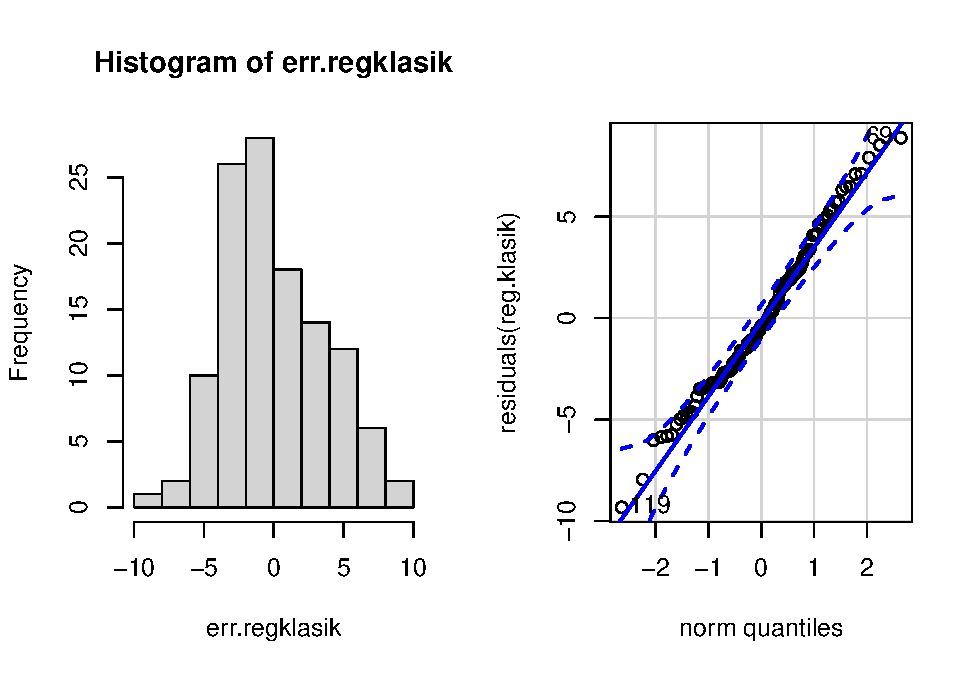
\includegraphics{modul_files/figure-latex/unnamed-chunk-56-1.pdf}

Sebagai ilustrasi, peubah rata-rata lama sekolah akan digunakan untuk memodelkan kemiskinan di pulau Jawa. Sebagai langkah awal, kita akan terlebih dulu memodelkannya menggunakan regresi linear.

\begin{Shaded}
\begin{Highlighting}[]
\NormalTok{fit.lm\textless{}{-}}\KeywordTok{lm}\NormalTok{(Kemiskinan}\OperatorTok{\textasciitilde{}}\NormalTok{Rata.Rata.Lama.Sekolah, }\DataTypeTok{data=}\NormalTok{datajawa)}
\KeywordTok{summary}\NormalTok{(fit.lm)}
\end{Highlighting}
\end{Shaded}

\begin{verbatim}
## 
## Call:
## lm(formula = Kemiskinan ~ Rata.Rata.Lama.Sekolah, data = datajawa)
## 
## Residuals:
##     Min      1Q  Median      3Q     Max 
## -7.0384 -1.9865 -0.3389  1.6722  9.7042 
## 
## Coefficients:
##                        Estimate Std. Error t value Pr(>|t|)    
## (Intercept)             24.7340     1.3417   18.44   <2e-16 ***
## Rata.Rata.Lama.Sekolah  -1.8657     0.1624  -11.49   <2e-16 ***
## ---
## Signif. codes:  0 '***' 0.001 '**' 0.01 '*' 0.05 '.' 0.1 ' ' 1
## 
## Residual standard error: 2.898 on 117 degrees of freedom
## Multiple R-squared:  0.5302, Adjusted R-squared:  0.5262 
## F-statistic:   132 on 1 and 117 DF,  p-value: < 2.2e-16
\end{verbatim}

Selanjutnya, diagnostik model dilakukan untuk memeriksa pemenuhan asumsi pada model regresi linear.

\begin{Shaded}
\begin{Highlighting}[]
\NormalTok{err.lm\textless{}{-}}\KeywordTok{residuals}\NormalTok{(fit.lm)}
\KeywordTok{shapiro.test}\NormalTok{(err.lm)}
\end{Highlighting}
\end{Shaded}

\begin{verbatim}
## 
##  Shapiro-Wilk normality test
## 
## data:  err.lm
## W = 0.98029, p-value = 0.07818
\end{verbatim}

\begin{Shaded}
\begin{Highlighting}[]
\KeywordTok{par}\NormalTok{(}\DataTypeTok{mfrow=}\KeywordTok{c}\NormalTok{(}\DecValTok{1}\NormalTok{,}\DecValTok{2}\NormalTok{))}
\KeywordTok{hist}\NormalTok{(err.lm)}
\NormalTok{car}\OperatorTok{::}\KeywordTok{qqPlot}\NormalTok{(}\KeywordTok{residuals}\NormalTok{(fit.lm))}
\end{Highlighting}
\end{Shaded}

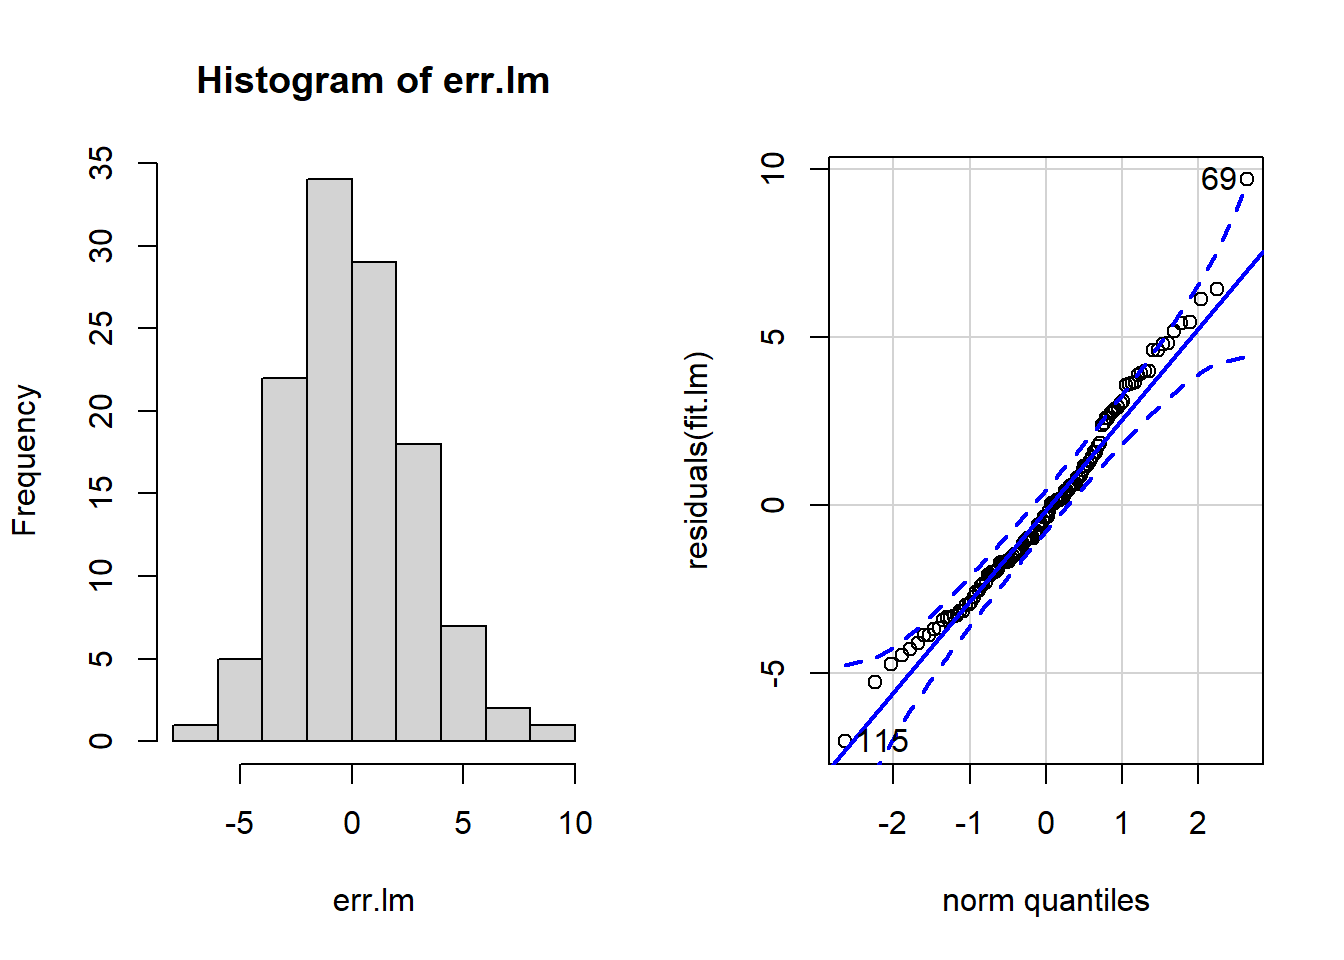
\includegraphics{modul_files/figure-latex/unnamed-chunk-58-1.pdf}

\begin{verbatim}
## [1]  69 115
\end{verbatim}

\begin{Shaded}
\begin{Highlighting}[]
\KeywordTok{plot}\NormalTok{(fit.lm,}\DataTypeTok{which=}\DecValTok{1}\NormalTok{)}
\NormalTok{lmtest}\OperatorTok{::}\KeywordTok{bptest}\NormalTok{(fit.lm)}
\end{Highlighting}
\end{Shaded}

\begin{verbatim}
## 
##  studentized Breusch-Pagan test
## 
## data:  fit.lm
## BP = 4.7982, df = 1, p-value = 0.02849
\end{verbatim}

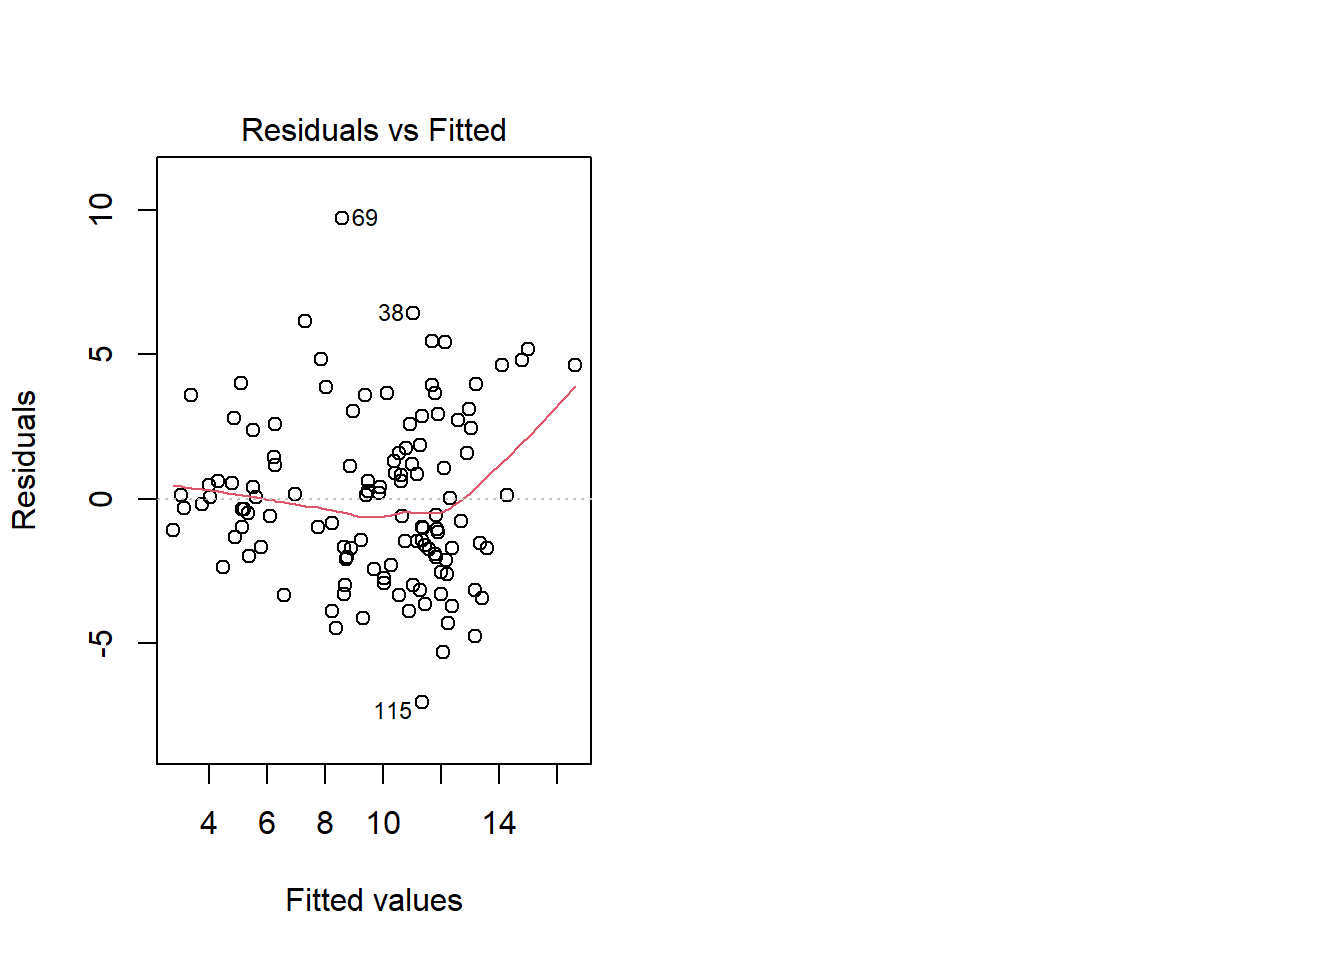
\includegraphics{modul_files/figure-latex/unnamed-chunk-58-2.pdf}

Terlihat pada output di atas bahwa sisaan model cenderung memiliki ragam yang tidak konstan. Selanjutnya juga akan diperiksa kebebasan sisaan menggunakan uji moran.

\begin{Shaded}
\begin{Highlighting}[]
\KeywordTok{library}\NormalTok{(spdep)}
\NormalTok{w\textless{}{-}}\KeywordTok{poly2nb}\NormalTok{(petajawa)}
\NormalTok{ww\textless{}{-}}\KeywordTok{nb2listw}\NormalTok{(w, }\DataTypeTok{zero.policy=}\NormalTok{T)}

\KeywordTok{lm.morantest}\NormalTok{(fit.lm, ww, }\DataTypeTok{alternative=}\StringTok{"two.sided"}\NormalTok{, }\DataTypeTok{zero.policy =}\NormalTok{ T)}
\end{Highlighting}
\end{Shaded}

\begin{verbatim}
## 
##  Global Moran I for regression residuals
## 
## data:  
## model: lm(formula = Kemiskinan ~ Rata.Rata.Lama.Sekolah, data =
## datajawa)
## weights: ww
## 
## Moran I statistic standard deviate = 5.9602, p-value = 2.519e-09
## alternative hypothesis: two.sided
## sample estimates:
## Observed Moran I      Expectation         Variance 
##       0.38842759      -0.01284003       0.00453256
\end{verbatim}

Terlihat pada output bahwa terdapat autokorelasi spasial pada sisaan model regresi linier. Dengan mempertimbangkan bahwa sisaan model memiliki ragam yang tidak homogen, serta memiliki autokorelasi spasial, kita selanjutnya dapat mencoba memodelkannya dengan model regresi terboboti geografis atau GWR. Namun pada modul pembelajaran ini, kami akan perlihatkan pula bahwa pada pemodelan regresi spasial pun ternyata tetap menghasilkan sisaan dengan ragam yang heterogen.

\begin{Shaded}
\begin{Highlighting}[]
\NormalTok{LM\textless{}{-}}\KeywordTok{lm.LMtests}\NormalTok{(fit.lm, ww,}\DataTypeTok{test=}\KeywordTok{c}\NormalTok{(}\StringTok{"LMerr"}\NormalTok{, }\StringTok{"LMlag"}\NormalTok{,}\StringTok{"RLMerr"}\NormalTok{,}\StringTok{"RLMlag"}\NormalTok{,}\StringTok{"SARMA"}\NormalTok{), }\DataTypeTok{zero.policy=}\NormalTok{T)}
\KeywordTok{summary}\NormalTok{(LM)}
\end{Highlighting}
\end{Shaded}

\begin{verbatim}
##  Lagrange multiplier diagnostics for spatial dependence
## data:  
## model: lm(formula = Kemiskinan ~ Rata.Rata.Lama.Sekolah, data =
## datajawa)
## weights: ww
##  
##         statistic parameter   p.value    
## LMerr  32.3011683         1 1.320e-08 ***
## LMlag  18.2380122         1 1.949e-05 ***
## RLMerr 14.0653693         1 0.0001766 ***
## RLMlag  0.0022132         1 0.9624773    
## SARMA  32.3033815         2 9.670e-08 ***
## ---
## Signif. codes:  0 '***' 0.001 '**' 0.01 '*' 0.05 '.' 0.1 ' ' 1
\end{verbatim}

\begin{Shaded}
\begin{Highlighting}[]
\KeywordTok{library}\NormalTok{(spatialreg)}
\NormalTok{sem\textless{}{-}}\KeywordTok{errorsarlm}\NormalTok{(Kemiskinan}\OperatorTok{\textasciitilde{}}\NormalTok{Rata.Rata.Lama.Sekolah,}\DataTypeTok{data=}\NormalTok{datajawa,ww, }\DataTypeTok{zero.policy=}\NormalTok{T)}
\NormalTok{sar\textless{}{-}}\KeywordTok{lagsarlm}\NormalTok{(Kemiskinan}\OperatorTok{\textasciitilde{}}\NormalTok{Rata.Rata.Lama.Sekolah,}\DataTypeTok{data=}\NormalTok{datajawa,ww, }\DataTypeTok{zero.policy=}\NormalTok{T)}
\NormalTok{gsm\textless{}{-}}\KeywordTok{sacsarlm}\NormalTok{(Kemiskinan}\OperatorTok{\textasciitilde{}}\NormalTok{Rata.Rata.Lama.Sekolah,}\DataTypeTok{data=}\NormalTok{datajawa,ww, }\DataTypeTok{zero.policy=}\NormalTok{T)}

\KeywordTok{bptest.sarlm}\NormalTok{(sem)}
\end{Highlighting}
\end{Shaded}

\begin{verbatim}
## 
##  studentized Breusch-Pagan test
## 
## data:  
## BP = 5.6364, df = 1, p-value = 0.01759
\end{verbatim}

\begin{Shaded}
\begin{Highlighting}[]
\KeywordTok{bptest.sarlm}\NormalTok{(sar)}
\end{Highlighting}
\end{Shaded}

\begin{verbatim}
## 
##  studentized Breusch-Pagan test
## 
## data:  
## BP = 4.0536, df = 1, p-value = 0.04408
\end{verbatim}

\begin{Shaded}
\begin{Highlighting}[]
\KeywordTok{bptest.sarlm}\NormalTok{(gsm)}
\end{Highlighting}
\end{Shaded}

\begin{verbatim}
## 
##  studentized Breusch-Pagan test
## 
## data:  
## BP = 3.8557, df = 1, p-value = 0.04958
\end{verbatim}

\hypertarget{basic-gwr}{%
\section{Basic GWR}\label{basic-gwr}}

Kita dapat menggunakan fungsi \texttt{gwr} pada package \texttt{spgwr} untuk menyusun model GWR pada R software, seperti pada program berikut ini.

\begin{Shaded}
\begin{Highlighting}[]
\KeywordTok{library}\NormalTok{(spgwr)}
\end{Highlighting}
\end{Shaded}

\begin{verbatim}
## Warning: package 'spgwr' was built under R version 4.0.3
\end{verbatim}

\begin{verbatim}
## NOTE: This package does not constitute approval of GWR
## as a method of spatial analysis; see example(gwr)
\end{verbatim}

\begin{Shaded}
\begin{Highlighting}[]
\KeywordTok{coordinates}\NormalTok{(datajawa)\textless{}{-}}\KeywordTok{c}\NormalTok{(}\StringTok{"Longitude"}\NormalTok{,}\StringTok{"Latitude"}\NormalTok{)}
\NormalTok{gwr20 \textless{}{-}}\StringTok{ }\KeywordTok{gwr}\NormalTok{(Kemiskinan}\OperatorTok{\textasciitilde{}}\NormalTok{Rata.Rata.Lama.Sekolah,}\DataTypeTok{data=}\NormalTok{datajawa,}\DataTypeTok{bandwidth=}\DecValTok{20}\NormalTok{)}
\NormalTok{gwr20}
\end{Highlighting}
\end{Shaded}

\begin{verbatim}
## Call:
## gwr(formula = Kemiskinan ~ Rata.Rata.Lama.Sekolah, data = datajawa, 
##     bandwidth = 20)
## Kernel function: gwr.Gauss 
## Fixed bandwidth: 20 
## Summary of GWR coefficient estimates at data points:
##                           Min. 1st Qu.  Median 3rd Qu.    Max.  Global
## X.Intercept.           24.6607 24.6971 24.7366 24.7620 24.8026 24.7340
## Rata.Rata.Lama.Sekolah -1.8708 -1.8673 -1.8651 -1.8617 -1.8585 -1.8657
\end{verbatim}

Kita dapat pula mengganti bandwidth sesuai dengan yang diinginkan. Selanjutnya kita akan bandingkan perbedaan akibat penentuan bandwidth yang berbeda-beda tersebut.

\begin{Shaded}
\begin{Highlighting}[]
\NormalTok{gwr3 \textless{}{-}}\StringTok{ }\KeywordTok{gwr}\NormalTok{(Kemiskinan}\OperatorTok{\textasciitilde{}}\NormalTok{Rata.Rata.Lama.Sekolah,}\DataTypeTok{data=}\NormalTok{datajawa, }\DataTypeTok{bandwidth=}\DecValTok{3}\NormalTok{)}
\NormalTok{gwr3}
\end{Highlighting}
\end{Shaded}

\begin{verbatim}
## Call:
## gwr(formula = Kemiskinan ~ Rata.Rata.Lama.Sekolah, data = datajawa, 
##     bandwidth = 3)
## Kernel function: gwr.Gauss 
## Fixed bandwidth: 3 
## Summary of GWR coefficient estimates at data points:
##                           Min. 1st Qu.  Median 3rd Qu.    Max.  Global
## X.Intercept.           21.8567 23.3823 24.6838 25.4191 26.4774 24.7340
## Rata.Rata.Lama.Sekolah -2.0218 -1.8937 -1.8219 -1.7275 -1.6145 -1.8657
\end{verbatim}

\begin{Shaded}
\begin{Highlighting}[]
\NormalTok{gwr2 \textless{}{-}}\StringTok{ }\KeywordTok{gwr}\NormalTok{(Kemiskinan}\OperatorTok{\textasciitilde{}}\NormalTok{Rata.Rata.Lama.Sekolah,}\DataTypeTok{data=}\NormalTok{datajawa,}\DataTypeTok{bandwidth=}\DecValTok{2}\NormalTok{)}
\NormalTok{gwr2}
\end{Highlighting}
\end{Shaded}

\begin{verbatim}
## Call:
## gwr(formula = Kemiskinan ~ Rata.Rata.Lama.Sekolah, data = datajawa, 
##     bandwidth = 2)
## Kernel function: gwr.Gauss 
## Fixed bandwidth: 2 
## Summary of GWR coefficient estimates at data points:
##                           Min. 1st Qu.  Median 3rd Qu.    Max.  Global
## X.Intercept.           19.5961 22.5941 24.3392 25.7094 27.7499 24.7340
## Rata.Rata.Lama.Sekolah -2.1862 -1.9058 -1.7441 -1.6570 -1.4305 -1.8657
\end{verbatim}

\begin{Shaded}
\begin{Highlighting}[]
\NormalTok{betabw20 \textless{}{-}}\StringTok{ }\NormalTok{gwr20}\OperatorTok{$}\NormalTok{SDF}\OperatorTok{$}\NormalTok{Rata.Rata.Lama.Sekolah}
\NormalTok{betabw3 \textless{}{-}}\StringTok{ }\NormalTok{gwr3}\OperatorTok{$}\NormalTok{SDF}\OperatorTok{$}\NormalTok{Rata.Rata.Lama.Sekolah}
\NormalTok{betabw2 \textless{}{-}}\StringTok{ }\NormalTok{gwr2}\OperatorTok{$}\NormalTok{SDF}\OperatorTok{$}\NormalTok{Rata.Rata.Lama.Sekolah}
\KeywordTok{boxplot}\NormalTok{(betabw20, betabw3, betabw2, }\DataTypeTok{names=}\KeywordTok{c}\NormalTok{(}\StringTok{"bw=20"}\NormalTok{,}\StringTok{"bw=3"}\NormalTok{,}\StringTok{"bw=2"}\NormalTok{))}
\end{Highlighting}
\end{Shaded}

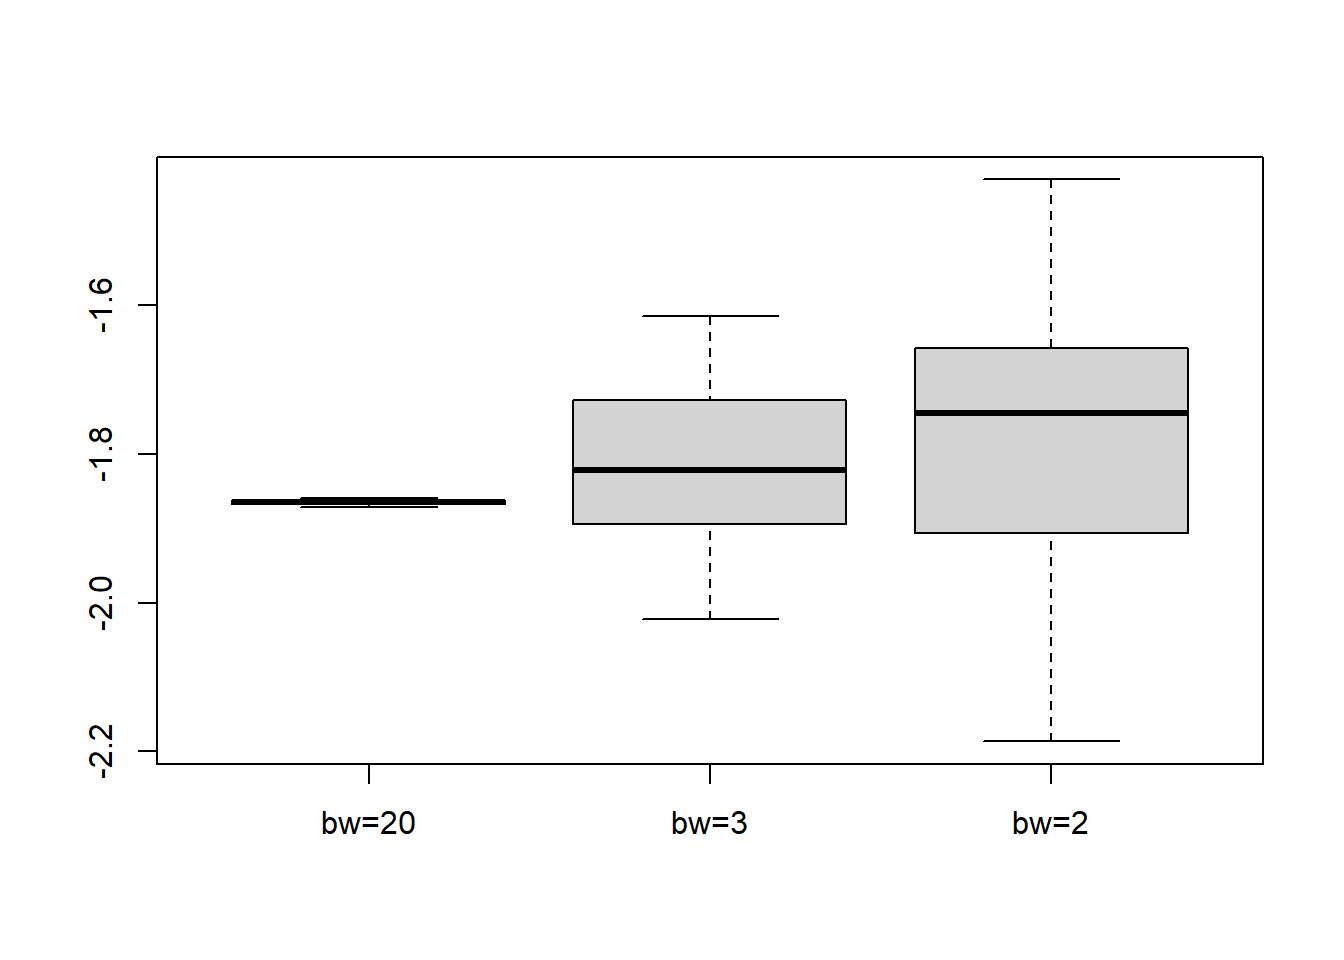
\includegraphics{modul_files/figure-latex/unnamed-chunk-65-1.pdf}

Output di atas memperlihatkan bahwa bandwidth yang lebih besar cenderung menghasilkan penduga koefisien model dengan rentang nilai yang lebih sempit. Sebaliknya, jika bandwidth yang digunakan lebih kecil, maka penduga koefisien model cenderung memiliki rentang nilai yang lebih lebar.

\hypertarget{menentukan-bandwidth-optimal}{%
\section{Menentukan Bandwidth Optimal}\label{menentukan-bandwidth-optimal}}

Penentuan bandwidth yang optimal dapat ditentukan berdasarkan kriteria AIC atau CV. Selain itu, kita juga dapat memilih fungsi pembobot kernel yang ingin digunakan pada pemodelan GWR.

\begin{Shaded}
\begin{Highlighting}[]
\NormalTok{bw1 \textless{}{-}}\StringTok{ }\KeywordTok{gwr.sel}\NormalTok{(Kemiskinan}\OperatorTok{\textasciitilde{}}\NormalTok{Rata.Rata.Lama.Sekolah,}\DataTypeTok{data=}\NormalTok{datajawa) }\CommentTok{\# default method is CV}
\end{Highlighting}
\end{Shaded}

\begin{verbatim}
## Bandwidth: 3.450257 CV score: 946.7623 
## Bandwidth: 5.577059 CV score: 985.8033 
## Bandwidth: 2.135821 CV score: 877.1735 
## Bandwidth: 1.323454 CV score: 806.2682 
## Bandwidth: 0.8213845 CV score: 752.5299 
## Bandwidth: 0.5110882 CV score: 697.962 
## Bandwidth: 0.3193146 CV score: 699.4435 
## Bandwidth: 0.4257648 CV score: 686.988 
## Bandwidth: 0.4182171 CV score: 686.7128 
## Bandwidth: 0.4036248 CV score: 686.6801 
## Bandwidth: 0.3714212 CV score: 689.1402 
## Bandwidth: 0.4101954 CV score: 686.6098 
## Bandwidth: 0.4102361 CV score: 686.6098 
## Bandwidth: 0.4101547 CV score: 686.6098 
## Bandwidth: 0.4076605 CV score: 686.62 
## Bandwidth: 0.410114 CV score: 686.6098 
## Bandwidth: 0.4101547 CV score: 686.6098
\end{verbatim}

\begin{Shaded}
\begin{Highlighting}[]
\NormalTok{gwr01 \textless{}{-}}\StringTok{ }\KeywordTok{gwr}\NormalTok{(Kemiskinan}\OperatorTok{\textasciitilde{}}\NormalTok{Rata.Rata.Lama.Sekolah,}\DataTypeTok{data=}\NormalTok{datajawa,}\DataTypeTok{bandwidth=}\NormalTok{bw1)}

\NormalTok{bw2 \textless{}{-}}\StringTok{ }\KeywordTok{gwr.sel}\NormalTok{(Kemiskinan}\OperatorTok{\textasciitilde{}}\NormalTok{Rata.Rata.Lama.Sekolah,}\DataTypeTok{data=}\NormalTok{datajawa,}\DataTypeTok{method=}\StringTok{"aic"}\NormalTok{)}
\end{Highlighting}
\end{Shaded}

\begin{verbatim}
## Bandwidth: 3.450257 AIC: 587.2351 
## Bandwidth: 5.577059 AIC: 591.8688 
## Bandwidth: 2.135821 AIC: 578.5693 
## Bandwidth: 1.323454 AIC: 569.3341 
## Bandwidth: 0.8213845 AIC: 562.5431 
## Bandwidth: 0.5110882 AIC: 558.7068 
## Bandwidth: 0.3193146 AIC: 575.363 
## Bandwidth: 0.6296109 AIC: 559.226 
## Bandwidth: 0.5177358 AIC: 558.6444 
## Bandwidth: 0.5525482 AIC: 558.5357 
## Bandwidth: 0.5819835 AIC: 558.6792 
## Bandwidth: 0.547683 AIC: 558.531 
## Bandwidth: 0.5465411 AIC: 558.5307 
## Bandwidth: 0.5462381 AIC: 558.5307 
## Bandwidth: 0.5462788 AIC: 558.5307 
## Bandwidth: 0.5461974 AIC: 558.5307 
## Bandwidth: 0.5462381 AIC: 558.5307
\end{verbatim}

\begin{Shaded}
\begin{Highlighting}[]
\NormalTok{gwr02 \textless{}{-}}\StringTok{ }\KeywordTok{gwr}\NormalTok{(Kemiskinan}\OperatorTok{\textasciitilde{}}\NormalTok{Rata.Rata.Lama.Sekolah,}\DataTypeTok{data=}\NormalTok{datajawa,}\DataTypeTok{bandwidth=}\NormalTok{bw2)}

\NormalTok{bwbs1 \textless{}{-}}\StringTok{ }\KeywordTok{gwr.sel}\NormalTok{(Kemiskinan}\OperatorTok{\textasciitilde{}}\NormalTok{Rata.Rata.Lama.Sekolah,}\DataTypeTok{data=}\NormalTok{datajawa,}\DataTypeTok{gweight=}\NormalTok{gwr.bisquare)}
\end{Highlighting}
\end{Shaded}

\begin{verbatim}
## Bandwidth: 3.450257 CV score: 816.2604 
## Bandwidth: 5.577059 CV score: 893.215 
## Bandwidth: 2.135821 CV score: 765.5706 
## Bandwidth: 1.323454 CV score: 696.4003 
## Bandwidth: 0.8213845 CV score: 722.8235 
## Bandwidth: 1.323495 CV score: 696.395 
## Bandwidth: 1.633776 CV score: 719.824 
## Bandwidth: 1.421531 CV score: 697.7054 
## Bandwidth: 1.36793 CV score: 694.5978 
## Bandwidth: 1.355794 CV score: 694.4734 
## Bandwidth: 1.358597 CV score: 694.4715 
## Bandwidth: 1.357479 CV score: 694.4699 
## Bandwidth: 1.357438 CV score: 694.4699 
## Bandwidth: 1.357397 CV score: 694.4699 
## Bandwidth: 1.357438 CV score: 694.4699
\end{verbatim}

\begin{Shaded}
\begin{Highlighting}[]
\NormalTok{gwr03 \textless{}{-}}\StringTok{ }\KeywordTok{gwr}\NormalTok{(Kemiskinan}\OperatorTok{\textasciitilde{}}\NormalTok{Rata.Rata.Lama.Sekolah,}\DataTypeTok{data=}\NormalTok{datajawa,}\DataTypeTok{gweight=}\NormalTok{gwr.bisquare,}
    \DataTypeTok{bandwidth=}\NormalTok{bwbs1)}

\NormalTok{bwbs2 \textless{}{-}}\StringTok{ }\KeywordTok{gwr.sel}\NormalTok{(Kemiskinan}\OperatorTok{\textasciitilde{}}\NormalTok{Rata.Rata.Lama.Sekolah,}\DataTypeTok{data=}\NormalTok{datajawa,}
                 \DataTypeTok{gweight=}\NormalTok{gwr.bisquare,}\DataTypeTok{method=}\StringTok{"aic"}\NormalTok{)}
\end{Highlighting}
\end{Shaded}

\begin{verbatim}
## Bandwidth: 3.450257 AIC: 570.608 
## Bandwidth: 5.577059 AIC: 580.6548 
## Bandwidth: 2.135821 AIC: 564.1267 
## Bandwidth: 1.323454 AIC: 558.0575 
## Bandwidth: 0.8213845 AIC: 575.6082 
## Bandwidth: 1.633751 AIC: 558.9865 
## Bandwidth: 1.310745 AIC: 558.1617 
## Bandwidth: 1.435388 AIC: 557.6479 
## Bandwidth: 1.429706 AIC: 557.6416 
## Bandwidth: 1.420138 AIC: 557.6375 
## Bandwidth: 1.420321 AIC: 557.6375 
## Bandwidth: 1.420399 AIC: 557.6375 
## Bandwidth: 1.42044 AIC: 557.6375 
## Bandwidth: 1.420399 AIC: 557.6375
\end{verbatim}

\begin{Shaded}
\begin{Highlighting}[]
\NormalTok{gwr04 \textless{}{-}}\StringTok{ }\KeywordTok{gwr}\NormalTok{(Kemiskinan}\OperatorTok{\textasciitilde{}}\NormalTok{Rata.Rata.Lama.Sekolah,}\DataTypeTok{data=}\NormalTok{datajawa,}\DataTypeTok{gweight=}\NormalTok{gwr.bisquare,}
    \DataTypeTok{bandwidth=}\NormalTok{bwbs2)}
\end{Highlighting}
\end{Shaded}

\hypertarget{menentukan-model-terbaik}{%
\section{Menentukan Model Terbaik}\label{menentukan-model-terbaik}}

Penentuan model terbaik dapat ditentukan berdasarkan beberapa kriteria tertentu. Fungsi \texttt{gwr} memungkinkan kita untuk mengevaluasi model berdasarkan AIC dan global quasi-\(R^2\), dengan terlebih dulu menambahkan argumen \texttt{hatmatrix=TRUE}.

\begin{Shaded}
\begin{Highlighting}[]
\NormalTok{gwr01 \textless{}{-}}\StringTok{ }\KeywordTok{gwr}\NormalTok{(Kemiskinan}\OperatorTok{\textasciitilde{}}\NormalTok{Rata.Rata.Lama.Sekolah,}\DataTypeTok{data=}\NormalTok{datajawa,}
             \DataTypeTok{hatmatrix=}\NormalTok{T, }\DataTypeTok{bandwidth=}\NormalTok{bw1)}
\NormalTok{gwr01}
\end{Highlighting}
\end{Shaded}

\begin{verbatim}
## Call:
## gwr(formula = Kemiskinan ~ Rata.Rata.Lama.Sekolah, data = datajawa, 
##     bandwidth = bw1, hatmatrix = T)
## Kernel function: gwr.Gauss 
## Fixed bandwidth: 0.4101547 
## Summary of GWR coefficient estimates at data points:
##                            Min.  1st Qu.   Median  3rd Qu.     Max.  Global
## X.Intercept.           12.68449 18.33784 23.15972 26.20076 38.10046 24.7340
## Rata.Rata.Lama.Sekolah -4.20789 -2.05946 -1.55904 -1.22414 -0.46292 -1.8657
## Number of data points: 119 
## Effective number of parameters (residual: 2traceS - traceS'S): 34.33575 
## Effective degrees of freedom (residual: 2traceS - traceS'S): 84.66425 
## Sigma (residual: 2traceS - traceS'S): 2.291766 
## Effective number of parameters (model: traceS): 25.10699 
## Effective degrees of freedom (model: traceS): 93.89301 
## Sigma (model: traceS): 2.176225 
## Sigma (ML): 1.933067 
## AICc (GWR p. 61, eq 2.33; p. 96, eq. 4.21): 562.1913 
## AIC (GWR p. 96, eq. 4.22): 519.682 
## Residual sum of squares: 444.673 
## Quasi-global R2: 0.7874434
\end{verbatim}

Fungsi \texttt{gwr} memberikan nilai AIC dengan tiga pendekatan, sehingga kita memperoleh AICc, AICb, dan AICh.

\begin{Shaded}
\begin{Highlighting}[]
\NormalTok{gwr01}\OperatorTok{$}\NormalTok{results}\OperatorTok{$}\NormalTok{AICc}
\end{Highlighting}
\end{Shaded}

\begin{verbatim}
## [1] 569.1585
\end{verbatim}

\begin{Shaded}
\begin{Highlighting}[]
\NormalTok{gwr01}\OperatorTok{$}\NormalTok{results}\OperatorTok{$}\NormalTok{AICb}
\end{Highlighting}
\end{Shaded}

\begin{verbatim}
## [1] 562.1913
\end{verbatim}

\begin{Shaded}
\begin{Highlighting}[]
\NormalTok{gwr01}\OperatorTok{$}\NormalTok{results}\OperatorTok{$}\NormalTok{AICh}
\end{Highlighting}
\end{Shaded}

\begin{verbatim}
## [1] 519.682
\end{verbatim}

Model terbaik adalah yang memiliki nilai AIC terkecil (bisa juga negatif) dan nilai global quasi-\(R^2\) yang terbesar. Namun demikian, kriteria tersebut tidak memberikan informasi inferensia apapun terkait siginifikansi model GWR.

Beberapa pendekatan uji dapat dilakukan untuk menguji \(H_0\) yang menyatakan bahwa model GWR tidak lebih baik daripada model OLS (regresi linier klasik), seperti yang dapat dilihat pada program-program berikut ini.

\begin{Shaded}
\begin{Highlighting}[]
\KeywordTok{BFC02.gwr.test}\NormalTok{(gwr01)}
\end{Highlighting}
\end{Shaded}

\begin{verbatim}
## 
##  Brunsdon, Fotheringham & Charlton (2002, pp. 91-2) ANOVA
## 
## data:  gwr01
## F = 2.2103, df1 = 117.000, df2 = 84.664, p-value = 7.714e-05
## alternative hypothesis: greater
## sample estimates:
## SS OLS residuals SS GWR residuals 
##         982.8726         444.6730
\end{verbatim}

\begin{Shaded}
\begin{Highlighting}[]
\KeywordTok{BFC99.gwr.test}\NormalTok{(gwr01)}
\end{Highlighting}
\end{Shaded}

\begin{verbatim}
## 
##  Brunsdon, Fotheringham & Charlton (1999) ANOVA
## 
## data:  gwr01
## F = 3.169, df1 = 87.18, df2 = 96.67, p-value = 2.996e-08
## alternative hypothesis: greater
## sample estimates:
## SS GWR improvement   SS GWR residuals 
##           538.1996           444.6730
\end{verbatim}

\begin{Shaded}
\begin{Highlighting}[]
\KeywordTok{LMZ.F1GWR.test}\NormalTok{(gwr01)}
\end{Highlighting}
\end{Shaded}

\begin{verbatim}
## 
##  Leung et al. (2000) F(1) test
## 
## data:  gwr01
## F = 0.62521, df1 = 96.67, df2 = 117.00, p-value = 0.00875
## alternative hypothesis: less
## sample estimates:
## SS OLS residuals SS GWR residuals 
##         982.8726         444.6730
\end{verbatim}

\begin{Shaded}
\begin{Highlighting}[]
\KeywordTok{LMZ.F2GWR.test}\NormalTok{(gwr01)}
\end{Highlighting}
\end{Shaded}

\begin{verbatim}
## 
##  Leung et al. (2000) F(2) test
## 
## data:  gwr01
## F = 1.9813, df1 = 47.916, df2 = 117.000, p-value = 0.001549
## alternative hypothesis: greater
## sample estimates:
##   SS OLS residuals SS GWR improvement 
##           982.8726           538.1996
\end{verbatim}

Berdasarkan output di atas, seluruh uji menunjukkan nilai \(p\)-value yang lebih kecil daripada taraf nyata 0.05, artinya \(H_0\) dapat ditolak, dan kita dapat menyimpulkan bahwa model GWR lebih baik daripada OLS, pada taraf nyata 5\%.

\begin{Shaded}
\begin{Highlighting}[]
\KeywordTok{LMZ.F3GWR.test}\NormalTok{(gwr01)}
\end{Highlighting}
\end{Shaded}

\begin{verbatim}
## 
## Leung et al. (2000) F(3) test
## 
##                        F statistic Numerator d.f. Denominator d.f.     Pr(>)
## (Intercept)                 2.6985        46.6539            96.67 1.988e-05
## Rata.Rata.Lama.Sekolah      2.1191        25.3140            96.67  0.004783
##                           
## (Intercept)            ***
## Rata.Rata.Lama.Sekolah ** 
## ---
## Signif. codes:  0 '***' 0.001 '**' 0.01 '*' 0.05 '.' 0.1 ' ' 1
\end{verbatim}

\hypertarget{menginterpretasikan-hasil-pemodelan-gwr}{%
\section{Menginterpretasikan Hasil Pemodelan GWR}\label{menginterpretasikan-hasil-pemodelan-gwr}}

Koefisien model GWR bersifat lokal, sehingga nilai penduga koefisien akan diperoleh pada setiap titik pengamatan. Oleh karenanya, interpretasi model GWR seringkali dilakukan dengan membuat visualisasi dalam bentuk peta, baru kemudian menginterpretasikannya.

\begin{Shaded}
\begin{Highlighting}[]
\KeywordTok{str}\NormalTok{(gwr01}\OperatorTok{$}\NormalTok{SDF)}
\end{Highlighting}
\end{Shaded}

\begin{verbatim}
## Formal class 'SpatialPointsDataFrame' [package "sp"] with 5 slots
##   ..@ data       :'data.frame':  119 obs. of  12 variables:
##   .. ..$ sum.w                        : num [1:119] 7.49 14.3 13.86 13.78 13.72 ...
##   .. ..$ (Intercept)                  : num [1:119] 17.1 15.5 15.8 15.8 15.7 ...
##   .. ..$ Rata.Rata.Lama.Sekolah       : num [1:119] -1.21 -1.08 -1.11 -1.1 -1.09 ...
##   .. ..$ (Intercept)_se               : num [1:119] 3.52 2.76 2.79 2.83 2.85 ...
##   .. ..$ Rata.Rata.Lama.Sekolah_se    : num [1:119] 0.35 0.287 0.29 0.294 0.295 ...
##   .. ..$ gwr.e                        : num [1:119] 5.168 -0.198 0.191 0.206 -0.93 ...
##   .. ..$ pred                         : num [1:119] 6.81 3.03 2.95 3.38 4.32 ...
##   .. ..$ pred.se                      : num [1:119] 0.761 0.775 0.794 0.708 0.554 ...
##   .. ..$ localR2                      : num [1:119] 0.485 0.633 0.642 0.616 0.602 ...
##   .. ..$ (Intercept)_se_EDF           : num [1:119] 3.71 2.91 2.94 2.98 3 ...
##   .. ..$ Rata.Rata.Lama.Sekolah_se_EDF: num [1:119] 0.369 0.303 0.306 0.309 0.311 ...
##   .. ..$ pred.se                      : num [1:119] 0.801 0.816 0.836 0.746 0.583 ...
##   ..@ coords.nrs : num(0) 
##   ..@ coords     : num [1:119, 1:2] 107 107 107 107 107 ...
##   .. ..- attr(*, "dimnames")=List of 2
##   .. .. ..$ : chr [1:119] "1" "2" "3" "4" ...
##   .. .. ..$ : chr [1:2] "Longitude" "Latitude"
##   ..@ bbox       : num [1:2, 1:2] 105.69 -8.24 114.37 -5.8
##   .. ..- attr(*, "dimnames")=List of 2
##   .. .. ..$ : chr [1:2] "Longitude" "Latitude"
##   .. .. ..$ : chr [1:2] "min" "max"
##   ..@ proj4string:Formal class 'CRS' [package "sp"] with 1 slot
##   .. .. ..@ projargs: chr NA
\end{verbatim}

Beberapa nilai dapat diperoleh langsung dari output fungsi \texttt{gwr}, yaitu penduga koefisien, hasil prediksi model, serta \emph{local}-\(R^2\). Selanjutnya, interpretasi dapat disesuaikan dengan konteks penelitian.

\begin{Shaded}
\begin{Highlighting}[]
\NormalTok{petajawa}\OperatorTok{$}\NormalTok{beta\textless{}{-}gwr01}\OperatorTok{$}\NormalTok{SDF}\OperatorTok{$}\NormalTok{Rata.Rata.Lama.Sekolah}
\NormalTok{petajawa}\OperatorTok{$}\NormalTok{pred\textless{}{-}gwr01}\OperatorTok{$}\NormalTok{SDF}\OperatorTok{$}\NormalTok{pred}
\NormalTok{petajawa}\OperatorTok{$}\NormalTok{localR2\textless{}{-}gwr01}\OperatorTok{$}\NormalTok{SDF}\OperatorTok{$}\NormalTok{localR2}

\KeywordTok{spplot}\NormalTok{(petajawa, }\StringTok{"beta"}\NormalTok{, }\DataTypeTok{main=}\StringTok{"Penduga Koefisien Model GWR"}\NormalTok{)}
\end{Highlighting}
\end{Shaded}

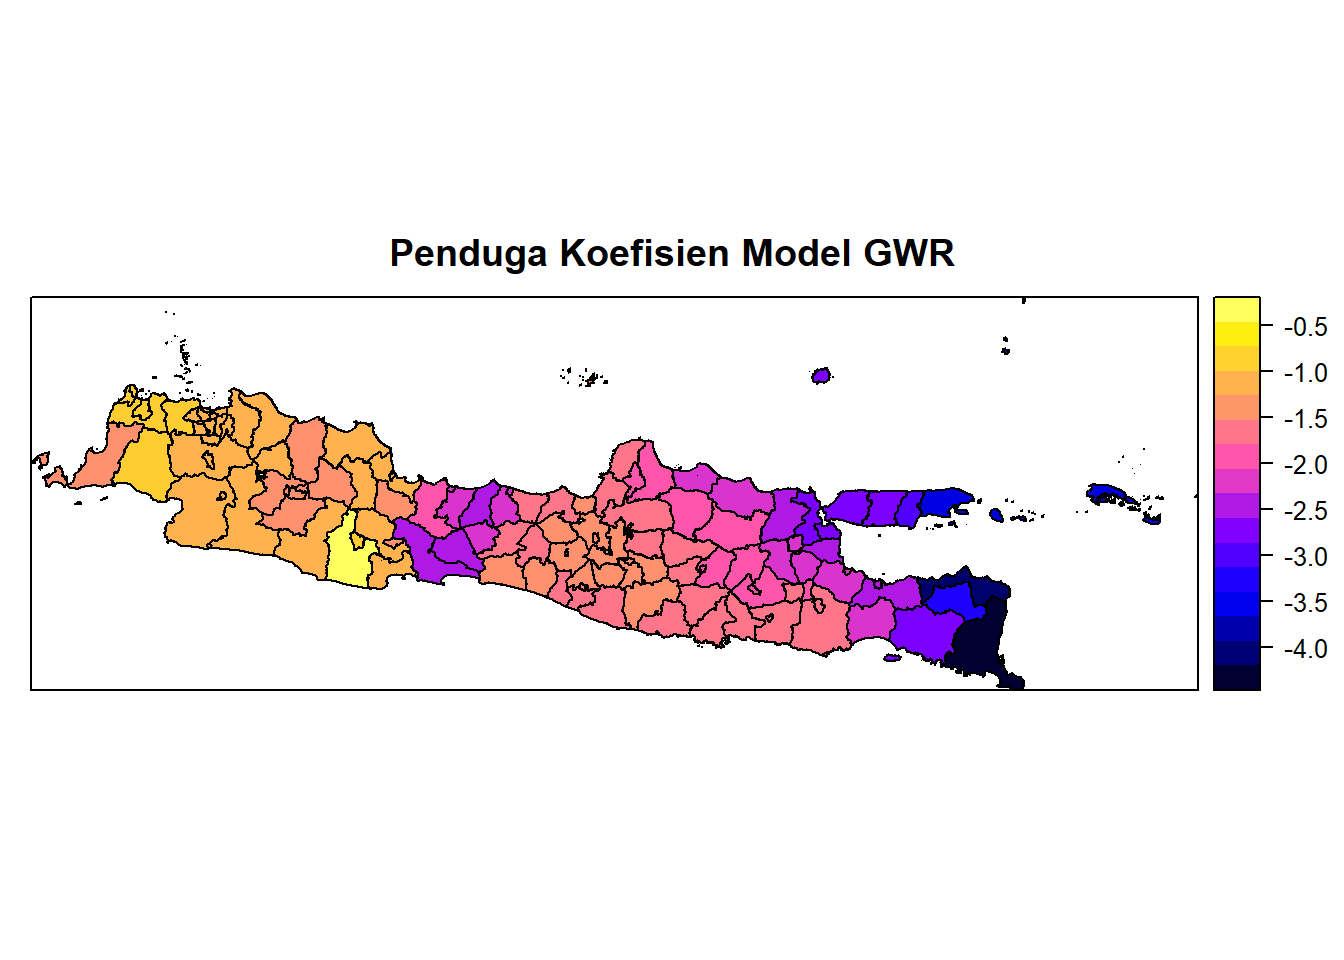
\includegraphics{modul_files/figure-latex/unnamed-chunk-75-1.pdf}

\begin{Shaded}
\begin{Highlighting}[]
\KeywordTok{spplot}\NormalTok{(petajawa, }\StringTok{"pred"}\NormalTok{, }\DataTypeTok{main=}\StringTok{"Prediksi Kemiskinan"}\NormalTok{)}
\end{Highlighting}
\end{Shaded}

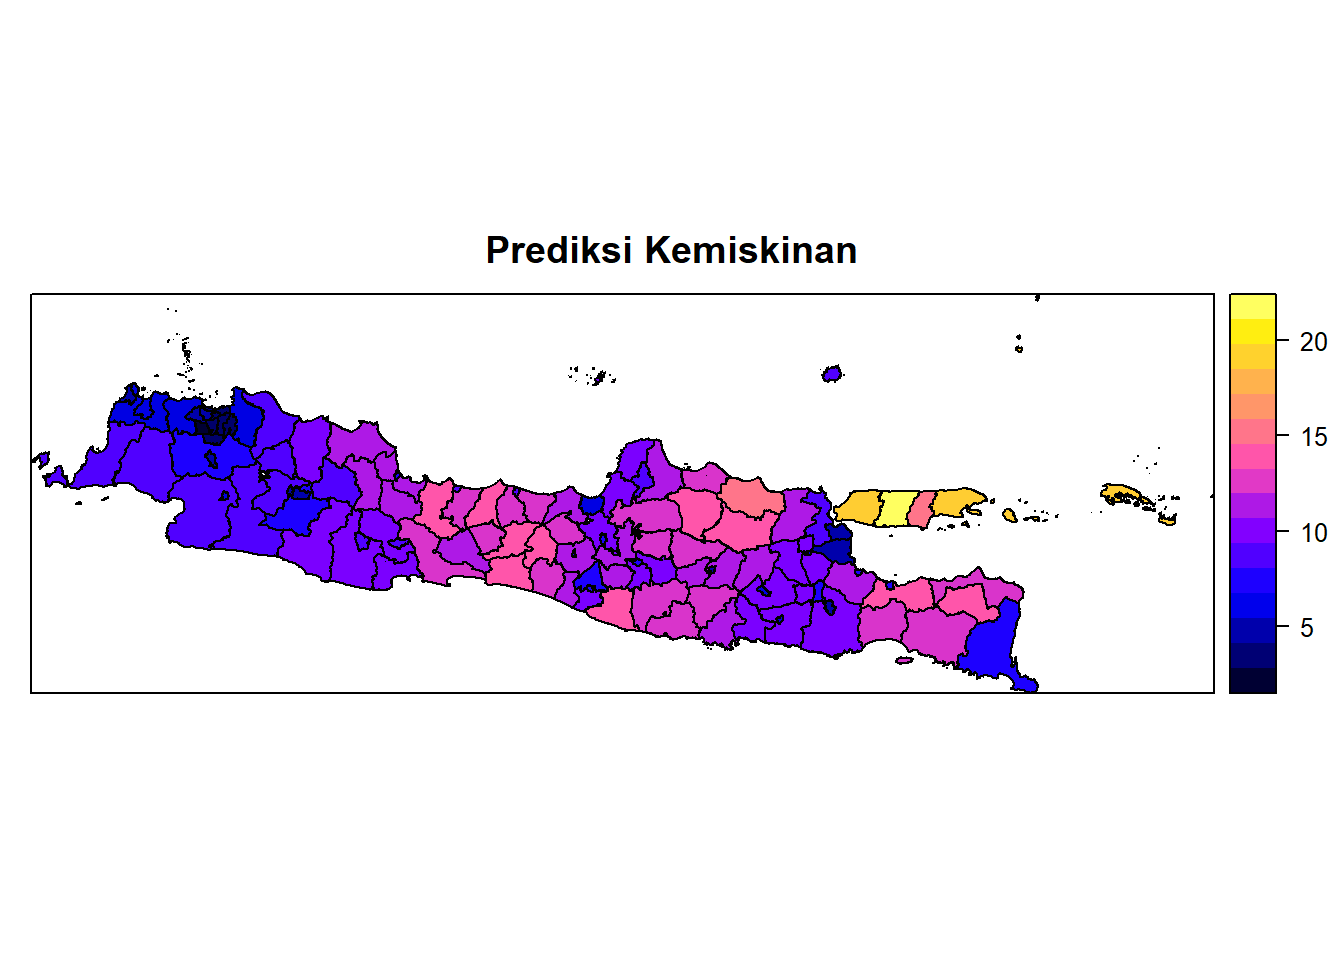
\includegraphics{modul_files/figure-latex/unnamed-chunk-75-2.pdf}

\begin{Shaded}
\begin{Highlighting}[]
\KeywordTok{spplot}\NormalTok{(petajawa, }\StringTok{"localR2"}\NormalTok{, }\DataTypeTok{main=}\StringTok{"Local R{-}square"}\NormalTok{)}
\end{Highlighting}
\end{Shaded}

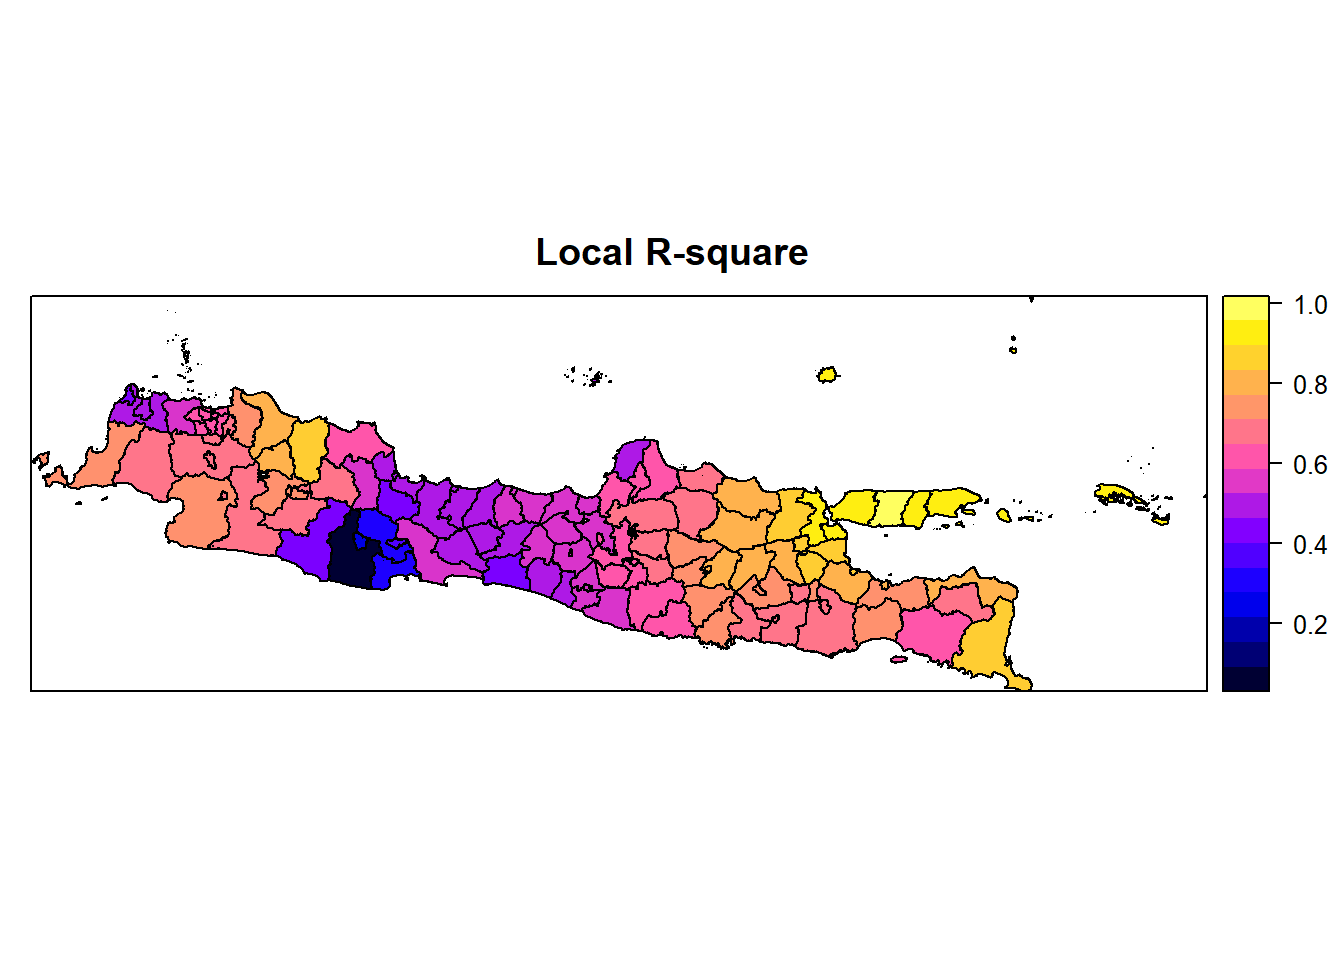
\includegraphics{modul_files/figure-latex/unnamed-chunk-75-3.pdf}

\hypertarget{sumber-pustaka-2}{%
\section{Sumber Pustaka}\label{sumber-pustaka-2}}

Brazil, N. (n.d.). Geographically weighted regression. CRD 230: Spatial Methods in Community Research. \url{https://crd230.github.io/gwr.html\#ordinary_least_squares_regression}

Brunsdon, C. 2015. Geographically Weighted Regression. \url{https://rstudio-pubs-static.s3.amazonaws.com/176883_06a3fa1fc77444be85e94dcd97ba9a34.html}

Dennett, A. (2014, November 17). An introduction to geographically weighted regression in R. \url{https://rstudio-pubs-static.s3.amazonaws.com/44975_0342ec49f925426fa16ebcdc28210118.html}

\hypertarget{applications}{%
\chapter{Applications}\label{applications}}

Some \emph{significant} applications are demonstrated in this chapter.

\hypertarget{example-one}{%
\section{Example one}\label{example-one}}

\hypertarget{example-two}{%
\section{Example two}\label{example-two}}

\hypertarget{final-words}{%
\chapter{Final Words}\label{final-words}}

We have finished a nice book.

  \bibliography{book.bib,packages.bib}

\end{document}
